\documentclass[12pt,a4paper]{book}
\usepackage[utf8]{inputenc}
\usepackage[spanish]{babel}
\usepackage{amsmath}
\usepackage{stackrel}
\usepackage{hyperref}
\usepackage[left=2.5cm,right=2.5cm,top=2cm,bottom=2.8cm]{geometry}
\setlength{\parskip}{4mm}

%\usepackage[linesnumbered,ruled,vlined]{algorithm2e}
\usepackage{wrapfig}
\usepackage{bm}
\usepackage{url}
%\PassOptionsToPackage{hyphens}{url} Permite que los enlaces URL puedan dividirse en múltiples líneas 
\usepackage{mathtools}
\usepackage{amsfonts}
\usepackage{amssymb}
\usepackage{esvect}
%\usepackage{subfig}
\usepackage{float}
\usepackage{enumitem}
%\usepackage{natbib}
\usepackage{amsthm}
\usepackage{graphicx}
\usepackage{xcolor}
\usepackage[nottoc]{tocbibind}
%\usepackage{synttree} 
\graphicspath{ {images/} }
\let\olditemize\itemize
\def\itemize{\olditemize\itemsep=0pt }
\setlength{\parindent}{0cm}
\setlist[itemize]{topsep=0pt}
\setlist[enumerate]{topsep=0pt}

\newtheorem{teo}{Teorema}[section]
\newtheorem{cor}[teo]{Corolario}
\newtheorem{defi}[teo]{Definición}
\newtheorem{prop}[teo]{Proposición}
\newtheorem{lema}[teo]{Lema}
\newtheorem{conj}[teo]{Conjetura}
\newtheorem{obs}[teo]{Observación}
\newtheorem{ejem}[teo]{Ejemplo}
\newtheorem{axioma}[teo]{Axioma}

\newcommand\Item[1][]{%
  \ifx\mathbb{R}lax#1\mathbb{R}lax  \item \else \item[#1] \fi
  \abovedisplayskip=-4pt\abovedisplayshortskip=0pt~\vspace*{-\baselineskip}}
% \DeclarePairedDelimiter{\abs}{\lvert}{\rvert} Define un nuevo comando \abs para facilitar la escritura de valores absolutos. Cuando uses \abs{x}, esto se representará como |x| con el tamaño de los delimitadores automáticamente ajustado al tamaño de x.

\newcommand{\mbb}{\mathbb}
\newcommand{\lp}{\ensuremath{\left(}}
\newcommand{\rp}{\ensuremath{\right)}}

%\usepackage[acronym]{glossaries}
\usepackage{multicol}
\usepackage{longtable}

\usepackage{listings}
\definecolor{codegreen}{rgb}{0,0.6,0}
\definecolor{codegray}{rgb}{0.5,0.5,0.5}
\definecolor{codepurple}{rgb}{0.58,0,0.82}
\definecolor{backcolour}{rgb}{0.95,0.95,0.92}
\lstdefinestyle{mystyle}{
    backgroundcolor=\color{backcolour},   
    commentstyle=\color{codegreen},
    keywordstyle=\color{magenta},
    numberstyle=\tiny\color{codegray},
    stringstyle=\color{codepurple},
    basicstyle=\ttfamily\footnotesize,
    breakatwhitespace=false,         
    breaklines=true,                 
    captionpos=b,                    
    keepspaces=true,                 
    numbers=left,                    
    numbersep=5pt,                  
    showspaces=false,                
    showstringspaces=false,
    showtabs=false,                  
    tabsize=2
}
\lstset{style=mystyle}


\usepackage{caption}
\usepackage{subcaption}

%\usepackage{fancyhdr}
%\pagestyle{fancy}
%\fancyhf{} % Limpia la cabecera y pie de página actuales
%\fancyhead[LO,RE]{\nouppercase{\leftmark}} % Cabecera de la página par (izquierda) e impar (derecha)
%\fancyhead[RO,LE]{\thepage} % Número de página en la cabecera derecha (páginas impares) y izquierda (páginas pares)
%\renewcommand{\headrulewidth}{0pt}
%\renewcommand{\chaptermark}[1]{%
%  \markboth{\chaptername\ \thechapter.\ #1}{}%
%}








\makeatletter
\newcommand{\dotminus}{\mathbin{\text{\@dotminus}}}

\newcommand{\@dotminus}{%
  \ooalign{\hidewidth\raise1ex\hbox{.}\hidewidth\cr$\m@th-$\cr}%
}
\makeatother


\usepackage{mdframed}
\newmdenv[leftline=false,topline=false]{topbot}
            
\author{Pablo Jiménez Poyatos}
\title{TFG}
\date{Julio 2024}


\makeglossaries
%\newacronym{uam}{UAM}{Urban Air Mobility}









\begin{document}

\pagenumbering{gobble}


\begin{titlepage}
		\centering
		
		{ \Large UNIVERSIDAD COMPLUTENSE DE MADRID}
		
		{ \Large \textbf{FACULTAD DE CIENCIAS MATEMÁTICAS}}
		\vspace{0.8cm}
		
		{ \large DEPARTAMENTO DE CIENCIAS DE LA  COMPUTACIÓN}
		\vspace{1cm}
		
		\vspace{0.6cm}
		
		\graphicspath{ {images/} }
		%%%%Logo Complutense%%%%%
		
\includegraphics[width=0.35\textwidth]{img/ucm.png} 
		\vspace{0.4cm}
		
        {\Large \textbf{TRABAJO DE FIN DE GRADO}}
		
		\vspace{8mm}
        {\huge \bfseries Algoritmos de Aprendizaje Automático aplicados a problemas de Ciberseguridad\par}
		\vspace{1cm}

		{\large Presentado por: Pablo Jiménez Poyatos}
		
		{\large Dirigido por: Luis Fernando Llana Diaz}
		
		\vspace{1.5cm}
		{\large Grado en Matemáticas}
		
		{\large Curso académico 2023-24}
\end{titlepage}

\thispagestyle{empty}
\clearpage
\setcounter{page}{1}


\newpage
\begin{center}
   {\bf Agradecimientos} 
\end{center}
%\begin{flushright}
%\textsl{A mi madre, lo hice por ti.}
%
%\textsl{A mi padre, para ser suficiente.}
%
%\textsl{A Sara y Yuki, la sístole y diástole de mi vida.}
%\end{flushright}
Estas páginas ponen punto y final a una de las etapas más complicadas de mi vida. Por eso, estos agradecimientos se van a quedar cortos.

En primer lugar, quiero agradecer y dedicar este trabajo a la sístole y diástole de mi vida. A mi compañera en lo bueno y en lo malo. Sara, infinitas gracias. Sin tu apoyo, no habría sido posible. Sin tu aliento, nunca habría podido llegar a la meta. Sin tu consejo, no habría encontrado la salida. Sin tu cariño y paciencia, esto no se habría podido materializar. Gracias y mil veces gracias. 

A mis padres, Ana y Francisco. Por dejarme decidir. Por confiar en mí. Ha sido un camino lleno de altibajos, de pensar que no se podía, que era demasiado difícil,... y lo fue, pero vosotros nunca me habéis exigido nada, y no puedo estar más agradecido y orgulloso de ser vuestro hijo. Desde aquella primera alegría desmesurada en el puerto de Gandía hasta hoy: ha sido todo por y para vosotros.

A mis amigos: Nacho, Sara, Marina y Rocío. De una u otra forma, sois parte de esto. Gracias por apoyarme siempre. 

A Julián, por darme y enseñarme las herramientas que han hecho esto posible. 

A mi gran y querido compañero de beca. Nunca pensé que sería becario en la universidad, pero si tuviera que repetir la experiencia, que fuera siempre contigo, Jhimmy. He aprendido y aprendo mucho de ti. Por muchas más charlas de programación, matemáticas e informática, y que nunca dejemos de construir castillos en el aire pensando en esas super empresas que se van a pelear por nosotros.

A mis compañeros del equipo de UTM en Indra, por resolver todas y cada una de mis dudas. En especial a Marta, por prestarse para la entrevista y guiar mis inicios como Ingeniero de Sistemas. 

A mi tutor, Rafa del Vado. Por su implicación desde aquel día que entró en el aula para darme clase, hasta el día en el que entrego esta memoria. Muchas gracias, eres una fuente de inspiración como matemático y como persona.  

Quiero mencionar también a algunas profesoras y profesores que han marcado mi camino: Pilar Cembranos, Rosa Alonso, Ángel Manuel Ramos, Ildefonso Díaz, Martín Avendaño, María del Mar Jiménez, Natalia López y Jose Luis Vega. Seguro que olvido a alguien. Han sido muchos los que han marcado este camino. Gracias por vuestra forma de trasmitir las matemáticas. 

A Rober Tomé por hacer las matemáticas accesibles. Por contar lo abstracto como si fuera una película. Gracias. 


  \textsl{Last but not least, I wanna thank me.}  
  \textsl{I wanna thank me for believing in me.}
  \textsl{I wanna thank me for doing all this hard work.} -
\textsl{Snoop Dogg}



 

\thispagestyle{empty}
\clearpage
\setcounter{page}{1}


\newpage
\begin{center}
   {\bf Resumen} 
\end{center}
El objetivo principal de esta investigación es la aplicación de los algoritmos genéticos al problema de diseño de vertipuertos. Basándonos en el estado del arte sobre diseño de vertipuertos y movilidad aérea urbana, complementado por las perspectivas obtenidas de una entrevista con una Ingeniera Aeroespacial experta en estos ámbitos, sentamos las bases del modelo matemático para el problema de óptimización, que resolveremos mediante heurísticas evolutivas, en concreto, algoritmos genéticos. Mediante un análisis de sensibilidad de los parámetros del algoritmo genético, hemos observado que tiende a converger hacia óptimos locales, lo cual destaca la necesidad de explorar estrategias adicionales para mejorar su capacidad de búsqueda global.    

\vspace{0.6 cm}
\textsl{\textbf{Palabras clave:} Vertipuerto, Algoritmos Genéticos, Óptimización, Heurísticas evolutivas, Movilidad Aérea Urbana.} 



\begin{center}
   {\bf Abstract} 
\end{center}

The main objective of this research is the application of genetic algorithms to the vertiport design problem. Based on the state of the art in vertiport design and urban air mobility, complemented by the insights obtained from an interview with an Aerospace Engineer expert in these areas, we establish the foundations of the mathematical model for the optimization problem that we will solve using evolutionary heuristics, specifically, genetic algorithms. Through a sensitivity analysis of the genetic algorithm parameters, we have observed that it tends to converge towards local optima, which highlights the need to explore additional strategies to improve its global search capability.


\vspace{0.6 cm}
\textsl{\textbf{Keywords:} Vertiport, Genetic Algorithms, Optimization, Evolutionary Heuristics, Urban Air Mobility.} 


\newpage
\tableofcontents

\newpage
\clearpage
\pagenumbering{arabic}
\chapter{Introducción} \label{Capitulo 1}
Las ciudades modernas enfrentan el reto de la movilidad urbana a diario y desde diferentes puntos de vista. No solo la congestión de sus carreteras forma parte de la problemática, las consideraciones sobre ecología y salud deben estar también presentes en los planes de movilidad de cualquier gran ciudad. En este primer capítulo, vamos a definir el concepto de \textsl{movilidad aérea urbana}, una posible solución integral al problema, ahondando en la infraestructura protagonista de este tipo de movilidad. Introduciremos el reto que supone diseñarla y hacer de ella una infraestructura eficiente desde el punto de vista de la optimización matemática. Finalmente, describiremos la estructura de la memoria, así como sus contribuciones más importantes. Las principales fuentes de consulta que han servido para la elaboración de este capítulo son: \cite{espejo-diaz_heuristic_2023, gupta_two-stage_1988, levitt_uam_2021, park_vertiport_2022}.       

\section{Motivación y objetivos del trabajo} \label{Sec:1_1}
Durante mis primeros meses de trabajo como Ingeniero de Sistemas en la división de UTM (de sus siglas en inglés, \textsl{Unmanned Traffic Management}) en Indra Sistemas S.A., me destinaron a uno de los proyectos europeos más ambiciosos en los que se está trabajando bajo el consorcio SESAR RJU\footnote{Para más información \url{https://www.sesarju.eu}.}: EUREKA \cite{proyEUREKA}. En este proyecto se están definiendo los flujos de trabajo dentro de vertipuertos, que es para los drones lo que un aeropuerto es para un avión, pero me llamó la atención que las diferentes infraestructuras que lo conforman no se colocaban según un cierto criterio. 

El problema que vamos a tratar en esta memoria se conoce como el \textsl{problema de diseño de vertipuertos}. Su objetivo principal es encontrar el diseño \textsl{óptimo} de un vertipuerto basándose en la geometría del espacio que se ha elegido para su construcción, en términos de maximizar la capacidad y el beneficio neto del operador del vertipuerto. Por tanto, enfrentamos un \textsl{problema de óptimización matemática} de interés, que surge para abordar un problema complejo en el sector aeroespacial. El problema trata de encontrar la posición óptima de las infraestructuras del vertipuerto, incluyendo las áreas de aterrizaje y despegue, puertas, calles de rodaje y terminales de pasajeros dentro del espacio delimitado para su instalación. Además, el sector se caracteriza por un estándar muy exigente en cuanto a los \textsl{requisitos de seguridad operacional}. Por todo ello, el uso de \textsl{algoritmos de optimización exactos} enfrenta varios retos relativos a la complejidad computacional, ya que las posibles soluciones crecen de manera exponencial, como los retos \textsl{hardware}, donde es necesario ser capaz de encontrar un balance óptimo entre tiempos de cómputo y una solución factible.

Este tipo de problemas tiene un gran número de variables y posibles combinaciones de la solución. Por ello, su complejidad computacional es NP-difícil \cite{espejo-diaz_heuristic_2023}, los algoritmos exactos suponen una mala elección a la hora de buscar el equilibrio del que hablábamos anteriormente.  

Sin embargo, estos retos suponen también una oportunidad única para aplicar {\sl heurísticas evolutivas}: algoritmos flexibles que se aplican a una gran variedad de problemas; estos algoritmos son robustos, ya que pueden encontrar buenas soluciones en espacios complejos con múltiples óptimos locales; permiten restricciones de diversos tipos, lo cual se hace indispensable cuando modelamos un problema real. Así mismo, permite incorporar el conocimiento experto que se tiene de un problema concreto: dado lo novedoso del problema, a tratar en este trabajo, el uso de estas técnicas heurísticas es también un camino sin recorrer, lo cual hace todavía más interesante su estudio.

Motivada la elección de la temática del trabajo nos planteamos partir de los siguientes objetivos: 
\begin{itemize}
	\item Asimilar conceptos complejos sobre movilidad aérea urbana y el negocio UTM. 
	\item Aprender sobre las heurísticas evolutivas para poder llevar a cabo la implementación correcta y eficiente de un algoritmo genético. 
	\item Aplicar y evolucionar mis conocimientos sobre Python. 
	\item Que dicha implementación sea capaz de obtener soluciones factibles en un tiempo razonable, con el fin de extraer conclusiones sobre su validez.
	\item Tratar de mejorar la solución ofrecida en el artículo \cite{yu_introduction_2010}, donde se propone un problema de diseño de vertipuertos \textsl{mediante programación entera}. 
	\item Trabajar otros problemas del negocio UTM, como puede ser el \textsl{problema de flujos de operación en un vertipuerto}, que introduciremos en la subsección \ref{Subsec: 1_2_3}. 
	\item Investigar y aprender sobre el mejor ajuste de configuración en algoritmos bioinspirados, como los algoritmos genéticos. 
	\item Realizar un estudio de sensibilidad que permita incrementar la calidad de las soluciones, sus trazas de validez, y su aplicabilidad a otros posibles escenarios que involucren el manejo de una mayor cantidad de información.  
\end{itemize}  
    
\section{Contexto y antecedentes del trabajo} \label{Sec:1_2}
En esta subsección vamos a introducir formalmente los conceptos de \textsl{movilidad aérea urbana}, \textsl{vertipuertos} y \textsl{optimización heurística}, además del \textsl{problema de optimización de diseño de un vertipuerto}.

 
\subsection{Movilidad Aérea Urbana} \label{Subsubsec: 1_2_1}
El futuro de la movilidad urbana pasa por utilizar medios de trasporte que nos permitan desplazarnos en un entorno fuertemente congestionado. Se prevé que más de 340 millones de personas vivan en entornos urbanos para 2030 \cite{easa_what_nodate}. La \textsl{Movilidad Aérea Urbana} (UAM, de sus siglas en inglés, \textsl{Urban Air Mobility}), es un concepto que propone una posible solución para que las urbes del futuro puedan afrontar el reto que supone la congestión del tráfico actual \cite{park_vertiport_2022}. Se trata de un nuevo sistema de transporte aéreo, que puede ser utilizado tanto por personas como para trasportar cargas. En este sentido, está especialmente orientada a operar en zonas densamente pobladas, y en un entorno con una gran cantidad de obstáculos. El progreso de los vehículos de propulsión eléctrica que despegan de forma vertical (eVTOL, de sus siglas en inglés, \textsl{electric Vertical Take-Off and Landing}), sugiere que este tipo de movilidad está cada vez más cerca de ser una realidad \cite{espejo-diaz_heuristic_2023}.  

La \textsl{Agencia Europea de Seguridad en la Aviación} (EASA, de sus siglas en inglés, \textsl{European Union Aviation Safety}) espera que la movilidad aérea urbana se convierta en una realidad en un plazo de 3 a 5 años. Baterías con más capacidad, redes 5G y nuevas tecnologías aplicadas al despegue vertical van a hacer posible su desarrollo.

Para gestionar este futuro próximo, una nueva infraestructura va a ser sin duda necesaria en nuestras ciudades, dando lugar a conceptos como el de los 
\textsl{vertipuertos}. Estos serán complejos dotados de las herramientas necesarias para llevar a cabo todas las fases operacionales de los eVTOL, como el almacenaje, recarga de baterías, aterrizaje, despegue y gestión de pasajeros y/o cargamento. 

Este trabajo pretende abordar el uso de la optimización heurística como herramienta para resolver los problemas asociados al diseño y gestión de los vertipuertos. Debido a la dimensión de estos problemas, utilizar esta herramienta permitirá buscar soluciones en tiempos computacionalmente asumibles y sin necesidad de explorar a fuerza bruta todas y cada una de las posibilidades, en base a un conocimiento experto del problema particular abordado.  



\subsection{Vertipuertos} \label{Subsec: 1_2_2}
Las regulaciones europeas trabajan para que este tipo de operación UAM comience y finalice en un vertipuerto \cite{easa_vertiports_2022}. Por este motivo, empresas privadas, organismos públicos y académicos, están dedicando recursos económicos y humanos en el desarrollo de lo que será la infraestructura principal de los sistemas UAM. Los vertipuertos, por tanto, serán centros para aeronaves eVTOL, como los taxis aéreos o los drones. 

Según la EASA, un vertipuerto se define como: \textsl{``Un área de tierra o agua o una estructura utilizadas, o previstas para ser utilizadas, para el aterrizaje y el despegue de aeronaves VTOL''} \cite{easa_verti_web}.

Un vertipuerto consiste en un \textsl{lado aire} y un \textsl{lado tierra}. El lado tierra contendrá la terminal de pasajeros, mientras que el lado aire, incluirá diferentes infraestructuras. Entre ellas, las principales son:

    \begin{enumerate}
    	\item \textbf{FATO}: de sus siglas, en inglés, \textsl{Final Approach and TakeOff}, son zonas de aproximación y despegue.
    	\item  \textbf{Puerta de embarque}: zonas que permiten aparcar, recargar las baterías, el mantenimiento de la aeronave, y la carga y descarga de pasajeros u otros elementos.
    	\item \textbf{Calles de rodadura} (o \textsl{zona de taxi}\footnote{Esta expresión viene del inglés, ya que ``hacer taxi'', en este idioma, hace referencia a una aeronave que se desplaza por el suelo utilizando su tren de aterrizaje.}): zonas de ruta a lo largo del vertipuerto para que la aeronave pueda desplazarse entre las zonas FATO y las puertas de embarque.
	\end{enumerate}       
   
Dependiendo de la localización del vertipuerto, existen: 
    \begin{enumerate}
    	\item \textbf{Vertipuertos dentro de un aeropuerto}: quedarían alejados de las pistas de la aviación tripulada del aeropuerto, pero dentro de las instalaciones.
     	\item \textbf{Vertipuertos en superficie}: construidos sobre un terreno a la altura del suelo. 
     	\item \textbf{Vertipuertos en cubierta}: en este caso, estarían a la altura del suelo, pero elevados gracias a una estructura que podría permitir, por ejemplo, un aparcamiento disuasorio\footnote{Estacionamiento ubicado en la corona metropolitana de las ciudades para aquellos pasajeros que intentan acceder al centro de la ciudad.} bajo ella. 
     	\item \textbf{Vertipuertos en altura}: construidos sobre algún tipo de edificación como, hospitales o centros comerciales. 
    \end{enumerate}
    
En este trabajo, partiremos de suponer la localización y el tamaño del vertipuerto como dados.

 \begin{wrapfigure}{r}{0.5\textwidth}
  \begin{center}
    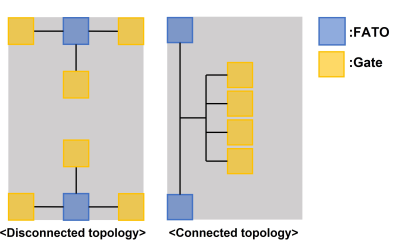
\includegraphics[width=0.48\textwidth]{img/tipos_topologia.png}
  \end{center}
    \caption{Tipos de \textsl{topologías} \cite{park_vertiport_2022}.}
  \label{fig:topologia_verti}
\end{wrapfigure}

Finalmente, introducimos la \textsl{topología del vertipuerto}, es decir, cómo aseguramos que las FATO están interconectadas con las puertas de embarques mediante calles de rodadura. En este punto, encontramos dos grandes familias: 

	\begin{enumerate}
		\item \textbf{Diseño desconectado}: en este caso, las calles de rodadura se utilizan sólo para conectar cada zona FATO con las diferentes puertas de embarque. De este modo, las FATO no están conectadas entre sí.  
    \item \textbf{Diseño conectado}: todo queda interconectado mediante las calles de rodadura, existiendo caminos entre los diferentes FATO con los que cuenta el vertipuerto.  
	\end{enumerate}
Podemos ver un croquis de ambas situaciones en la Figura \ref{fig:topologia_verti}.

%\begin{figure}[h]
%    \begin{center}
%    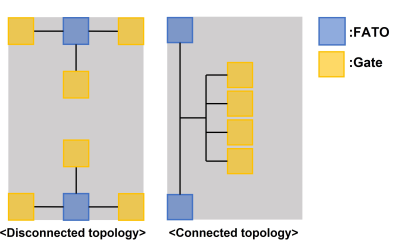
\includegraphics[width=0.4\textwidth]{img/tipos_topologia.png}
%    \end{center}
%    \caption{Tipos de \textsl{topologías} \cite{park_vertiport_2022}.}
%    \label{fig:topologia_verti}
%\end{figure} 

En este trabajo, optaremos por un diseño conectado. 
\subsection{Optimización del diseño de un vertipuerto} \label{Subsec: 1_2_3}
Como nueva infraestructura que formará parte de nuestras ciudades, el vertipuerto presenta varios retos. En este trabajo se han abordado los siguientes: 

\begin{itemize}
	\item Optimización de su diseño.
	\item Optimización de la planificación.  
\end{itemize}

En ambos casos, la optimización se hará sobre la figura principal del vertipuerto, su \textsl{operador}, ya sea para maximizar su beneficio o para mejorar la toma de decisiones de su personal. Definiremos el \textsl{operador del vertipuerto} como la entidad responsable de la gestión segura y eficiente de los recursos del vertipuerto. El \textsl{operador} del vertipuerto puede tener autoridad sobre la capacidad del operador UAM para aterrizar y despegar \cite{levitt_uam_2021}. Los trabajos que se han consultado para fundamentar los objetivos de esta memoria, \cite{park_vertiport_2022, espejo-diaz_heuristic_2023}, proponen la utilización de una optimización heurística para dar respuesta a ambos problemas.  

Más concretamente, los autores de \cite{park_vertiport_2022} buscan maximizar el beneficio neto del operador del vertipuerto. Para ello, en primer lugar, se debe elegir una ubicación geográfica. Esta debe ser próxima a áreas donde se exprima el potencial del UAM. Estas áreas representan varios retos, como el elevado precio del suelo y una densidad urbana que se caracteriza por una concentración notable de edificaciones, entre las cuales se encuentran algunas construcciones notablemente altas. Por esto, los vertipuertos deben diseñarse optimizando tanto el espacio como la seguridad. Asumiendo que la localización, el tamaño y la forma (topología) vienen dados, el problema radica en encontrar su diseño óptimo, respetando a su vez las \textsl{condiciones de seguridad}. 

Durante las operaciones que se llevan a cabo en un vertipuerto, las aeronaves invierten tiempo, por ejemplo, a la hora de embarcar o desembarcar pasajeros. Cada infraestructura de las que conforman un vertipuerto tiene asociado un tiempo de servicio. Dependiendo de las infraestructuras que posea el vertipuerto, este tendrá unos tiempos de servicio que determinarán su capacidad. Igualmente, las operaciones que se llevan a cabo en las FATO dependerán de ciertos criterios de seguridad, como, por ejemplo, la separación mínima entre aeronaves. Por ello, es importante equilibrar también el número de infraestructuras que posee el vertipuerto para conseguir maximizar su rendimiento. En resumen, el número de infraestructuras y su correspondiente rendimiento determinarán la \textsl{capacidad en el lado aire}, que se define como el número estimado de operaciones en un determinado tiempo. Este tipo de restricciones se denominan \textsl{restricciones operacionales}.  

Finalmente, el diseño de vertipuertos tiene asociadas una serie de topologías tradicionales (lineal, satelital o embarcadero \cite{preis_quick_2021}). No obstante, estas topologías no responden adecuadamente a las demandas de seguridad y las restricciones asociadas a las infraestructuras. Por tanto, un VDP (de sus siglas en inglés \textsl{Vertiport Desing Problem}) buscará el diseño óptimo que maximice la capacidad y satisfaga las restricciones operacionales desde el principio del proyecto.

\begin{figure}[h]
    \begin{center}
    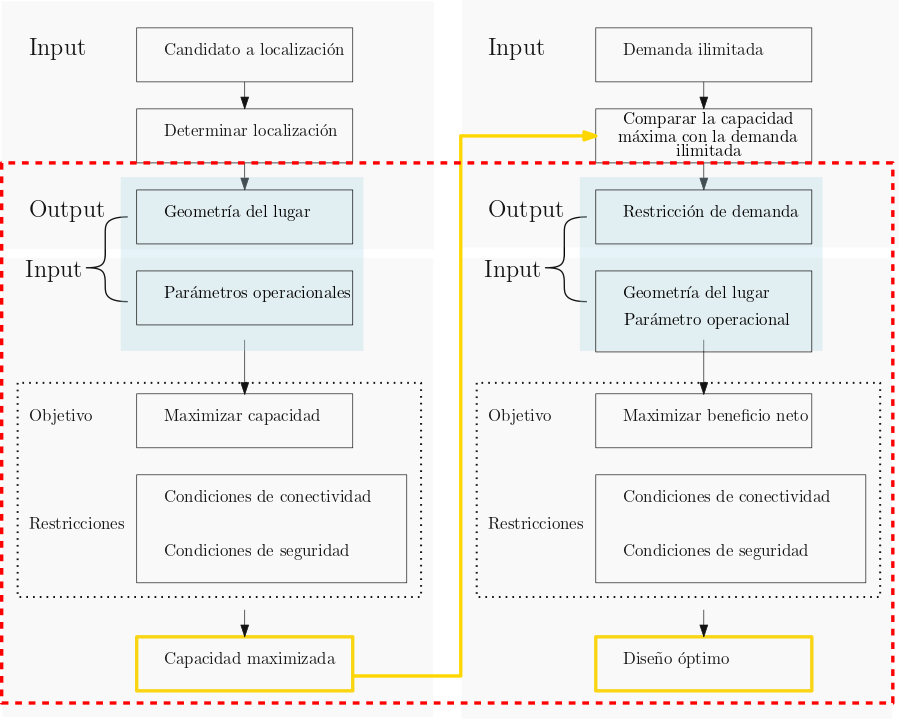
\includegraphics[width=0.8\textwidth]{img/proceso_diseno_vertipuerto.png}
    \end{center}
    \caption{Proceso de diseño de un vertipuerto y alcance del trabajo  \cite{park_vertiport_2022}.}
    \label{fig:proceso-diseño-VDP}
\end{figure} 

En la Figura \ref{fig:proceso-diseño-VDP} ilustramos en un diagrama los diferentes procesos que hemos mencionado hasta obtener el diseño óptimo. Podemos resumir el proceso en tres pasos, que, de acuerdo con \cite{park_vertiport_2022}, serían:  
\begin{enumerate}
	\item Identificar la \textsl{capacidad máxima del vertipuerto}. 
	\item Calcular las \textsl{restricciones de demanda}. Suponiendo que la demanda UAM es suficiente, de modo que las restricciones de demanda sean iguales a la capacidad máxima del vertipuerto. 
	\item Encontrar el diseño óptimo que permita \textsl{maximizar el beneficio neto} desde la perspectiva del operador del vertipuerto. 
\end{enumerate} 
Lo novedoso de estos trabajos radica en la idea de acomodar, dentro del modelo, las restricciones operacionales, mejorando la toma de decisiones del operador del vertipuerto, en contraposición a las topologías tradicionales. Además, contribuirá a realizar una previsión más precisa de la demanda UAM, ya que en estudios precedentes esta demanda se suponía sin restricción o aleatorizada. 

Por otro lado, el reto al que se hace frente en \cite{espejo-diaz_heuristic_2023} es la gestión del volumen de aeronaves que hacen uso de las instalaciones. En esta ocasión, la figura principal será el \textsl{Vertiport Manager} \cite{proyEUREKA}, en adelante VM, el cual aún se está definiendo con precisión. No obstante, sus funciones serán parecidas a las de un ATCO (de sus siglas en inglés \textsl{Air Traffic Control Officer}), limitadas al vertipuerto en el que desempeñe sus funciones. El objetivo será que las decisiones del VM se sustenten en metodologías que secuencien, de forma adecuada, el flujo de aeronaves entre las componentes del vertipuerto.

En este estudio, se presentan dos modelos matemáticos que, haciendo uso de la optimización heurística, pretenden optimizar las salidas y llegadas. Este problema consiste en asignar y secuenciar los eVTOL en las componentes del vertipuerto: calles de rodadura, FATO, etc. Para ello, se tienen en cuenta dos objetivos: 
\begin{itemize}
	\item Maximizar el rendimiento. 
	\item Minimizar la desviación del tiempo de llegada/salida respecto del que se había programado inicialmente.
\end{itemize} 
Se tienen en cuenta \textsl{condiciones operativas}, como la separación mínima entre eVTOL, o impedir que dos aeronaves ocupen la misma infraestructura de forma simultánea. Respecto a las componentes del vertipuerto introducidas en la subsección \ref{Subsec: 1_2_2}, los autores de \cite{espejo-diaz_heuristic_2023} introducen una zona que recuerda a los hangares de un aeropuerto tradicional, y que darían cabida a aquellos eVTOL que estén fuera de servicio. 

El esquema elegido es el de un diseño conectado, con una separación entre FATO que permite operaciones simultaneas. Se ha divido el vertipuerto en los siguientes 4 niveles: 
\begin{itemize}
	\item \textbf{Nivel 1}: Calle de rodadura 1.
	\item \textbf{Nivel 2}: Puertas de embarque. 
	\item \textbf{Nivel 3}: Calle de rodadura 2. 
	\item \textbf{Nivel 4}: FATO.
\end{itemize}


\begin{figure}[h]
    \begin{center}
    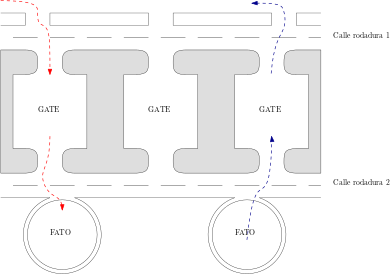
\includegraphics[width=0.6\textwidth]{img/proceso_verti.png}
    \end{center}
    \caption{Flujos de trabajo en un vertipuerto \cite{espejo-diaz_heuristic_2023}.}
    \label{fig:proceso-trabajo-verti}
\end{figure} 

Como se puede ver en la Figura \ref{fig:proceso-trabajo-verti} los eVTOL cuentan con dos operativas básicas: 
\begin{itemize}
	\item {\sl Marcada por las flechas rojas}. Esta operativa consiste en \textsl{hacer taxi} hasta el nivel 2 dónde recibirá la carga o se montarán los pasajeros y llegar hasta el nivel 4 para despegar.
	\item {\sl Marcada por las flechas azules}. Esta operativa es la opuesta a la anterior. La aeronave aterriza en el nivel 4, deposita la carga o los pasajeros en las \textsl{gates} y finalmente pasa a la zona de hangares.   
\end{itemize}

En cuanto a las restricciones que se plantean en este problema, destacamos: 
\begin{itemize}
	\item Dos aeronaves no pueden permanecer simultáneamente en la misma infraestructura dentro del vertipuerto, por razones de seguridad. Asimismo, deberán esperar que el componente esté disponible para transferirse a la siguiente zona. 
	\item Los autores denominan \textsl{restricciones de bloqueo} a aquellas situaciones en las que aeronaves con diferente propósito (salida vs. llegada) quieran ocupar la misma calle de rodadura, y quedan, por tanto, confrontadas. Finalmente, en la zona de despegue y aterrizaje (FATO), debe prevalecer un criterio de separación mínima. 
	\item Las limitaciones tecnológicas en las baterías de la aeronave hacen necesario añadir \textsl{restricciones relativas a los tiempos de carga}. 
	\item Posibles prioridades para aeronaves de los servicios de emergencia. 
\end{itemize}

De este modo, se introducen los problemas que se denominan HFS, de sus siglas en inglés \textsl{Hybrid Flowshop Scheduling}. Estos problemas plantean un entorno en el cual hay un conjunto de tareas que se deben realizar por etapas, de entre las cuales al menos una tendrá más de una \textsl{máquina de trabajo en paralelo}. 
\begin{itemize}
	\item En nuestro contexto, las máquinas en paralelo son las diferentes infraestructuras que conforman el vertipuerto. 
	\item Por otro lado, las aeronaves son los trabajos que deben ser asignados y secuenciados en las infraestructuras (máquinas). 
\end{itemize}

Presentados ambos problemas, cabe destacar que: 
\begin{itemize}
	\item El problema VDP queda dentro de los problemas de programación entera IP (de sus siglas en inglés \textsl{Integer Programing}) en los cuales el tiempo de cálculo aumenta exponencialmente a medida que el tamaño del problema se incrementa, debido a la naturaleza NP-difícil del problema de programación entera. 
	\item Los problemas HFS, que, en su mayoría de casos, son NP-difíciles \cite{espejo-diaz_heuristic_2023}. Esto se debe a que, incluso en configuraciones relativamente simples (como dos etapas de procesamiento, con dos máquinas en una etapa y una en la otra), el problema sigue siendo NP-difícil \cite{gupta_two-stage_1988}. 
\end{itemize}

En la siguiente subsección, \ref{Subsubsec: 1_2_4}, presentaremos la optimización heurística, siendo está una herramienta adecuada para enfrentar computacionalmente ambos problemas.

\subsection{Optimización heurística} \label{Subsubsec: 1_2_4}
La \textsl{optimización} es una herramienta matemática que ayuda, especialmente, en la toma de decisiones \cite{e_besada_optimizacion_nodate}. Perteneciente a la rama de la \textsl{Investigación Operativa}, forma parte de la vida cotidiana de cualquier empresa, y se utiliza para llegar a una decisión más o menos precisa con ayuda de un modelo matemático. Generalmente, estos problemas se resuelven de forma exacta, ya que se reducen a problemas mixtos de programación lineal, entera o cuadrática, para los que existe software comercial competente como \href{https://www.ibm.com/mx-es/products/ilog-cplex-optimization-studio/cplex-optimizer}{CPLEX} de la empresa IBM o \href{https://www.gurobi.com/}{Gurobi Optimization}. No obstante, algunos de estos problemas no permiten ser abordados mediante estas estrategias, debido a un coste computacional demasiado elevado \cite{e_besada_optimizacion_nodate, jorge_martinez_liebana_investigacion_2019}. 

Un \textsl{problema de optimización} está compuesto de \cite{e_besada_optimizacion_nodate}: 
\begin{itemize}
	\item Un conjunto de \textsl{variables de decisión} que representan los parámetros variables del problema.  
	\item Las \textsl{restricciones} las cuales nos dan relaciones entre las variables de decisión y sus valores, permitiendo diferenciar soluciones válidas de las que no lo son.   
	\item Las \textsl{funciones objetivo} son una representación matemática de los logros industriales que se desean conseguir.
\end{itemize}

Podemos entender, entonces, el proceso de optimización como aquel que trata de encontrar los valores de las variables de decisión que cumplan con todas las restricciones, y que \textsl{maximizan} o \textsl{minimizan} las funciones objetivo. Dependiendo de cómo estos valores se adapten al problema, tendremos diferentes tipos de soluciones \cite{e_besada_optimizacion_nodate}:
 
\begin{itemize}
	\item \textsl{Factible}: satisface todas las restricciones.
	\item \textsl{Óptima}: solución factible que alcanza el mejor valor posible de la función objetivo.
	\item \textsl{No factible}: no satisface alguna de las restricciones.
	\item \textsl{No acotada}: produce un valor de la función objetivo que tiende a infinito (\textsl{max.} o \textsl{min.} respectivamente).
\end{itemize}

Para dar respuesta a estos problemas, que suponen un coste computacional tan elevado, sería deseable encontrar soluciones factibles lo suficientemente buenas en un tiempo razonable. De esta forma, si bien el objetivo de esta disciplina matemática es encontrar el óptimo del problema, sacrificaríamos dicho valor por una aproximación suficientemente buena del óptimo, en favor de tiempos de cómputo más aceptables. Entre las técnicas capaces de resolver los problemas de esta forma destacan los \textsl{algoritmos de optimización heurística}. 

El término \textsl{heurística} proviene de la palabra griega \textsl{eureka}, cuyo significado está relacionado con el concepto de \textsl{encontrar}, el cual se vincula a la supuesta exclamación de Arquímedes (287 a.C. - 212 a.C.) al descubrir su famoso principio \cite{e_besada_optimizacion_nodate}. Según la RAE (Real Academia Española), la heurística se define como: 
\begin{quote}
\textsl{En algunas ciencias, manera de buscar la solución de un problema mediante métodos no rigurosos, como por tanteo, reglas empíricas, etc.}
\end{quote}
Estos conceptos serán tratados en el Capítulo \ref{Capitulo_2}. En este trabajo nos centraremos en un tipo concreto de algoritmo heurístico basado en la propia biología, los algoritmos genéticos, debido a que son particularmente útiles en problemas de optimización combinatoria debido a su capacidad para explorar eficientemente espacios de soluciones grandes y complejos, encontrando soluciones óptimas o casi óptimas cuando los métodos de búsqueda tradicionales pueden quedarse atrapados en óptimos locales o ser computacionalmente inviables.


%Es importante señalar que existen diferentes concepciones de lo que se entiende por heurística \cite{e_besada_optimizacion_nodate}: 
%\begin{itemize}
%	\item En Inteligencia Artificial el término heurística se utiliza para describir una técnica, método o procedimiento inteligente para llevar a cabo una tarea, que no se basa en un análisis formal estricto, sino en el conocimiento experto sobre la tarea. 
%	\item En Investigación Operativa se asocia con un procedimiento que habitualmente encuentra soluciones de alta calidad con un coste computacional razonable, pero que no garantiza ni la optimalizad ni factibilidad de las soluciones encontradas, ni es capaz de determinar lo lejos que está de alcanzarlas	. 
%	\end{itemize}
	
%[JLG: Comento esto a espera de que me confirmes que debe ser borrado] En el final de la sección anterior hemos hecho referencia a los problemas NP-Complejos y es que existen diferentes clasificaciones para los problemas de optimización. Uno de los criterios más habituales es la complejidad computacional. En base a este criterio clasificamos los problemas en dos grandes familias: 
%\begin{itemize}
%	\item Problemas de clase $\mathcal{P}$. Son aquellos para los que podemos hallar una solución en un tiempo que depende polinomialmente del tamaño del problema. Si tomamos $n$ como el tamaño del problema, expresamos su complejidad como $\mathcal{O}(P(n))$ donde $P(n)$ es el polinomio que asocia dicho tamaño al orden del tiempo de computo $\mathcal{O}(\bullet)$.
%	\item Problemas de clase $\mathcal{NP}$. En este caso no es posible encontrar una solución óptima en tiempo polinomial. Aquí encontramos dos grupos: 
%	\begin{itemize}
%		\item Problemas $\mathcal{NP}$-Complejos 
%		\item Problemas $\mathcal{NP}$-Completos 
%\end{itemize}	 
%En este caso se emplearán algoritmos que proporcionen una buena solución rápidamente aunque no garanticen la optimalidad.
%\end{itemize} 
%
%Como vimos en la sección \ref{Subsec: 1_2_3} nuestros problemas son $\mathcal{NP}$-complejos, que formalmente, se definen como: 
%
%\begin{defi}[\textsl{Problema $\mathcal{NP}$-complejo \cite{korte_combinatorial_2012}}] 
%Un problema computacional $\mathcal{P}$ es $\mathcal{NP}$-complejo si todos los problemas en $\mathcal{NP}$ se reducen polinomialmente a $\mathcal{P}$ . 
%\end{defi} 
%
%\begin{figure}[H]
%    \begin{center}
%    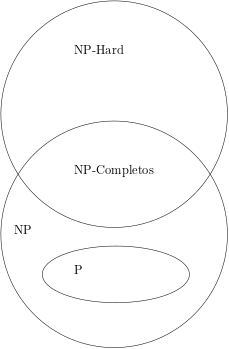
\includegraphics[width=0.3\textwidth]{img/np-problems.png}
%    \end{center}
%    \caption{Clasificación de problemas según su complejidad}
%    \label{fig:Np-problemas}
%\end{figure} 
%
%De este modo, queda motivado el uso que haremos de este tipos de técnicas para resolver los problemas de vertipuertos. }

\section{Estructura de la memoria} \label{Subsubsec: 1_3}
La memoria se ha estructurado en seis capítulos. El capítulo actual contiene una introducción dirigida tanto a motivar los objetivos del trabajo como a contextualizar el problema de estudio. En los capítulos \ref{Capitulo_2} y \ref{Capitulo_3} encontramos descripciones formales tanto de la optimización heurística, como del problema de vertipuertos. Posteriormente, en el Capítulo 4 se encuentran las bases de implementación para algoritmos genéticos en lenguaje Python que sirve, además, como explicación detallada de los algoritmos genéticos que hemos introducido anteriormente. El Capítulo \ref{Capítulo 5} se ha destinado a la puesta en práctica del algoritmo descrito en el Capítulo \ref{Capítulo 4} para la resolución del modelo presentado en el Capítulo \ref{Capitulo_3} con su correspondiente análisis. Finalizamos la memoria con un capítulo de conclusiones y la sugerencia de nuevas líneas de investigación derivadas del trabajo realizado. 

En el Apéndice \ref{app:entrevista} de esta memoria, encontraremos la transcripción de la entrevista previa realizada a una experta en UTM.  

\section{Contribuciones} \label{Subsec: 1_4}
El diseño de vertipuertos presenta un complejo desafío, ya que involucra múltiples criterios de optimización, que iremos abordando en este trabajo. Tradicionalmente, las metodologías para abordar este problema han recurrido a enfoques exactos, limitando así la exploración de soluciones innovadoras y óptimas en tiempos de cómputo igualmente eficientes. No obstante, la adopción de técnicas de optimización heurística marca un enfoque novedoso y prometedor, ofreciendo una metodología flexible y adaptable capaz de explorar el complejo espacio de soluciones posibles que nos brindan los problemas de optimización combinatoria.  Estas nuevas técnicas, como los algoritmos genéticos, permiten identificar configuraciones de diseño altamente eficientes con un mejor coste computacional.

Sin embargo, cabe reconocer que, al ser métodos aproximativos, la optimización heurística puede no siempre alcanzar la solución exacta con toda la precisión deseada. La naturaleza probabilística implica una aceptación del equilibrio entre la calidad de la solución y el tiempo computacional requerido. Además, la posibilidad de aplicar el conocimiento experto es vital cuando nos movemos en escenarios de diseño urbano, donde las variables de decisión y las restricciones pueden ser tan numerosas y complejas que la búsqueda de una solución exacta se vuelve, prácticamente, inviable.

En este trabajo se presenta una implementación en Python, completamente original, de un modelo matemático realista del VDP. Esta implementación puede servir para experimentar, comparar con otras soluciones algorítmicas y, también, como punto de partida para futuras investigaciones. 

Finalmente, en el desarrollo del modelo matemático que fundamenta este trabajo, he aplicado de manera integral los conocimientos y competencias adquiridos durante mi formación académica en el grado de Matemáticas. Esta base educativa ha sido esencial para abordar la complejidad del diseño, permitiéndome formular un modelo sólido que incorpora tanto principios de optimización como técnicas formales de programación.  Este enfoque ha permitido traducir requisitos prácticos y restricciones técnicas en formulaciones matemáticas, estableciendo así un puente entre la teoría matemática pura y su aplicación en la resolución de un problema realista. Particularmente relevante ha sido mi comprensión de la teoría de complejidad computacional y la naturaleza de los problemas NP-difíciles, adquirida durante mi grado. Este conocimiento ha sido indispensable para buscar estrategias de optimización eficientes. Este trabajo me ha enfrentado a un problema que permite valorar la alternativa a los métodos exactos adoptando un enfoque heurístico, en particular aplicando una estrategia novedosa, para los VDP, como los algoritmos genéticos. 

\chapter{Optimización Heurística} \label{Capitulo_2}
Este capítulo está dedicado a la optimización, en particular, a su vinculación con la rama de las heurísticas. Dedicaremos la atención a las \textsl{heurísticas evolutivas}, en concreto, a los \textsl{algoritmos genéticos}. Introduciremos, en primer lugar, esta técnica matemática desde el punto de vista histórico, presentando sus principales componentes, para, finalmente, describir su estructura general. Las principales fuentes de consulta que han servido para la elaboración del capítulo son \cite{cuevas_matlab_2021, e_besada_optimizacion_nodate, hooker_testing_1995, gparedes_hernandez_fundamentos_2021, linares_modelos_2001, silver_overview_2004}. 

\section{De la realidad a la solución} \label{Subsec: 3_1}
En la subsección \ref{Subsubsec: 1_2_4} comentamos brevemente los ingredientes principales de un problema de optimización, así como el concepto de \textsl{heurística}. Si bien conocer los esquemas de optimización es importante, que estos respondan a un \textsl{modelo} es crucial dentro de la disciplina. Según la RAE, este modelo se define como: 

\begin{quote}
\textsl{``Esquema teórico, generalmente en forma matemática, de un sistema o de una realidad compleja (por ejemplo, la evolución económica de un país), que se elabora para facilitar su comprensión y el estudio de su comportamiento.''}
\end{quote}

Modelar, por tanto, es la acción de construir un modelo, de ``encorsetar'' la realidad \cite{linares_modelos_2001}. Un modelo debe plantearse nivelando su cantidad de detalles con la factibilidad de encontrar alguna técnica para resolverlo. Su desarrollo se divide en las siguientes etapas: 

\begin{itemize}
	\item \textbf{Identificación del problema}. Consiste en buscar y analizar la información del problema. Hay que ser preciso, de forma que lo recopilado pueda expresarse en lenguaje matemático. Es una etapa fundamental, pues de ella depende la calidad de las conclusiones futuras. 
    \item \textbf{Especificación matemática y formulación}. Se escribe el problema de optimización definiendo sus variables, ecuaciones, función objetivo y parámetros. 
    \item \textbf{Resolución}. En esta etapa se utilizará un algoritmo para llegar a la solución numérica (idealmente cercana a la matemática) óptima o casi-óptima. Este algoritmo puede tener un propósito general (e.g., el {\sl método del Simplex}) o específico para el modelo. 
    \item \textbf{Verificación, validación y refinamiento}. En esta fase se pretende eliminar los errores que se hayan podido dar en la codificación (esto es, verificar). Es necesario comprobar la validez de las simplificaciones realizadas utilizando las soluciones obtenidas (esto es, validar), o comprobando que los resultados son coherentes en la realidad. 
    \item \textbf{Interpretar y analizar resultados}. Se proponen las soluciones. Se realiza un análisis de sensibilidad de los parámetros de entrada, lo que permite conocer el comportamiento del modelo. También se comprueba la robustez de la solución óptima. 
    \item\textbf{ Implementación, documentación y mantenimiento}. El objetivo de esta etapa es garantizar la difusión a través de una documentación clara, precisa y completa, así como un código bien documentado que facilite su mantenimiento.  
\end{itemize}

A su vez, en \cite{silver_overview_2004} se presenta, en la Figura \ref{fig:realPr_to_solution}, el uso de modelos matemáticos para ayudar en la toma de decisiones en situaciones del mundo real, y lo dividen en cuatro etapas:

\begin{figure}[h]
    \begin{center}
    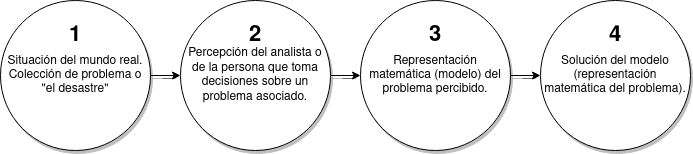
\includegraphics[width=0.8\textwidth]{img/problemToSolution.png}
    \end{center}
    \caption{De la situación real a la solución.}
    \label{fig:realPr_to_solution}
\end{figure} 

Finalmente, en este camino, necesitaremos dos ingredientes más: un conjunto de datos que permita crear las diferentes iteraciones del modelo, y saber de qué forma resolvemos el problema. Desgraciadamente, la complejidad del mundo real nos lleva a modelos igualmente complejos que no pueden ser abordados con métodos exactos. 
%
%En esta sección, se pretende profundizar en el concepto de optimización así como en el de optimización heurística como método para la resolución del problema planteado en el Capítulo \ref{Capitulo_3}. 
\section{Algoritmos exactos de optimización matemática} \label{Subsec: 3_2}
La \textsl{optimización} representa el proceso de encontrar la \textsl{mejor solución} a un problema entre un conjunto muy grande de soluciones posibles \cite{cuevas_matlab_2021}. La teoría de optimización clásica está enfocada en encontrar e identificar al mejor candidato de entre un conjunto de alternativas, sin evaluarlas explícitamente; por ello, un \textsl{problema de optimización} es, en general, un \textsl{problema de decisión} \cite{gparedes_hernandez_fundamentos_2021}.  

Un \textsl{problema de optimización} es un proceso donde se quiere encontrar el valor óptimo $\mathbf{x} = (x_1, \ldots, x_d) \in \mathbf{X}$ que \textsl{minimiza} o \textsl{maximiza} la función objetivo $f(\mathbf{x})$, donde $\mathbf{X}$ representa el conjunto de soluciones o \textsl{espacio de búsqueda}. Este espacio de búsqueda puede estar limitado inferiormente por el valor $l_i$, y superiormente por un valor $u_i$, de forma que $\mathbf{X} = \{ \mathbf{x} \in \mathbb{R}^d \, \vert \, l_i \leq x_i \leq u_i, \; i = 1, \ldots, d \}$. Finalmente, tendrá una serie de restricciones que pueden ser de desigualdad o de igualdad. Formalmente: 

\begin{align}
\min / \max \, \nonumber                               & \\ 
                                                                            & f(\mathbf{x}),  \; \mathbf{x} \in \mathbb{R}^n \nonumber \\
\text{sujeto a las restricciones } \nonumber & \\  
                                                                             & g_i(\mathbf{x}) \leq 0, \quad i = 1, \ldots, q \nonumber \\
                                                                             & h_j(\mathbf{x}) = 0, \quad j = q + 1, \ldots, k \nonumber \\
                                                                             & l_l \leq \mathbf{x}_l \leq u_l, \quad l = 1, \ldots, n \label{COPs}
\end{align}


%Los problemas de maximización y minimización se dicen equivalentes, ya que:
%
%\begin{align}
% \min_\mathbf{x} f(\mathbf{x}) \Leftrightarrow \max_\mathbf{x}[(-1) \cdot f(\mathbf{x})]\\
% \max_\mathbf{x} f(\mathbf{x}) \Leftrightarrow \min_\mathbf{x}[(-1) \cdot f(\mathbf{x})]
%\end{align}

Problemas de optimización hay tantos como formas de expresar $f(\mathbf{x})$. Las \textsl{técnicas de optimización} nos permiten encontrar el óptimo en el espacio de búsqueda mediante procesos iterativos. Existen dos grandes familias de algoritmos a los que vamos a hacer referencia en este capítulo: \textsl{esquemas clásicos} y \textsl{esquemas metaheurísticos}. 

Los métodos clásicos, como los \textsl{métodos Newtonianos}, utilizan el gradiente de la función $f(\mathbf{x})$ para el proceso de iteración, mientras que los métodos heurísticos, como los \textsl{algoritmos evolutivos}, ignoran la derivada y orientan la búsqueda gracias a unas \textsl{reglas} que permiten acotar y dirigir la exploración.  

%Veamos ahora, de forma rigurosa, cómo y de qué está compuesto un problema de optimización. Tal y como se presenta en \cite{e_besada_optimizacion_nodate}, la forma más general de un problema de optimización viene dada por

%\begin{equation}
%\begin{matrix}
%\text{opt}_{\mathbf{x}} G(f_1(\mathbf{x}), f_2(\mathbf{x}),\ldots, f_o(\mathbf{x}))\\
%\mathbf{x} = [x_1, x_2, \ldots, x_N] \\
%\mathbf{x} \in \Omega
%\end{matrix}
%\end{equation}



%donde
%\begin{itemize}
%	\item $\mathbf{x}$ representa el vector que contiene las $N$ variables de decisión del problema. 
%	\item $\Omega$ es el espacio sobre el que se encuentran definidas las soluciones factibles del problema. Este queda definido por el tipo $T$ asociado a cada variable y las relaciones matemáticas $g_i(\mathbf{x}) \leq 0$ y $h_k(\mathbf{x}) = 0$ que definen las restricciones del problema 
%	\begin{equation}
%	\mathbf{x} \in \Omega = \left \lbrace \begin{matrix}
%	x_i \in T_i \\
%	g_j(\mathbf{x}) \leq 0, j = 1,\ldots, R\\
%	h_k(\mathbf{x}) = 0, k = 1, \ldots, P
%\end{matrix}	\right. 
%	\end{equation}
%	\item $f_i(x)$ cada una de las $O$ funciones objetivo que define el problema de optimización. 
%	\item $\text{opt}_\mathbf{x}\, G(\bullet)$ el método utilizado para combinar y optimizar de forma simultánea todos los objetivos. 
%\end{itemize}
%
%Para resolver este problema podemos optimizar simultáneamente todos los objetivos. Los métodos que lo encaran de esta forman se pueden dividir en: 
%\begin{itemize}
%	\item Aquellos que convierten un problema con $O>1$ objetivos, en un problema con un único objetivo por medio de una combinación (generalmente lineal) de todos los objetivos. Por tanto, maximizan o minimizan el valor combinado. Por ejemplo, $\min_\mathbf{x} \sum_{i = 1}^O w_i\cdot f_i(\mathbf{x})$, donde se le da una importancia, un \textsl{peso} $w_i$, diferente a cada objetivo.
%	\item Aquellos que optimizan simultáneamente todos los objetivos del problema utilizando una definición en la que se establece si una solución es mejor que otra comparando cada uno de los objetivos por separado. Por ejemplo: Pareto optimalidad \cite{e_besada_optimizacion_nodate}. 
%\end{itemize}
%
%Este tipo de estrategia es un caso particular de aquellos problemas con múltiples objetivos en los que no necesariamente se utiliza la función $G(\bullet)$.
%
%
%Algunos conceptos fundamentales que se aplican a los problemas de optimización de forma general son: 
%
%\begin{itemize}
%	\item \textbf{Vector de decisión factible}: es aquel $\mathbf{x}$ que cumple las restricciones, esto es $\mathbf{x} \in \Omega$. 
%	\item \textbf{Óptimo local}: un vector de decisión factible $\mathbf{x}^*$ representa un óptimo local de la función  $G(f_1(\mathbf{x}),f_2(\mathbf{x}),\ldots, f_O(\mathbf{x}))$ si su valor en ese punto no es peor que el de sus vecinos; esto es, $\exists\, \varepsilon > 0$ tal que  $G(f_1(\mathbf{x}^*),f_2(\mathbf{x}^*),\ldots, f_O(\mathbf{x}^*))$ no es peor que $G(f_1(\mathbf{x}),f_2(\mathbf{x}),\ldots, f_O(\mathbf{x}))\, \forall \mathbf{x}$ factible en el entorno definido por$\parallel \mathbf{x}-\mathbf{x}^* \parallel < \varepsilon$, con la distancia usual. 
%	\item \textbf{Óptimo global}: un vector de decisión factible $\mathbf{x}^*$ representa un óptimo global de la función  $G(f_1(\mathbf{x}),f_2(\mathbf{x}),\ldots, f_O(\mathbf{x}))$ si su valor en ese punto no es peor que cualquier otro vector; esto es, si $G(f_1(\mathbf{x}^*),f_2(\mathbf{x}^*),\ldots, f_O(\mathbf{x}^*))$ no es peor que $G(f_1(\mathbf{x}),f_2(\mathbf{x}),\ldots,$ $f_O(\mathbf{x})),\, \forall \mathbf{x} \in \Omega$. 
%	\item \textbf{Punto de silla}: un vector de decisión factible $\mathbf{x}^*$ dividido en dos subvectores $[\mathbf{x}^*_a, \mathbf{x}_b^*]$ representa un punto de silla de la función $G(f_1(\mathbf{x}^*),f_2(\mathbf{x}^*),\ldots, f_O(\mathbf{x}^*))$ si en la vecindad de ese punto hay puntos factibles mejores y peores que él; esto es si $\exists \, \varepsilon > 0$: 
%\begin{equation}
%\, G(f_1([\mathbf{x}_a, \mathbf{x}_b^*]),f_2([\mathbf{x}_a, \mathbf{x}_b^*]),\ldots, f_O([\mathbf{x}_a, \mathbf{x}_b^*]))
%	\end{equation}	
%no es peor que 
%\begin{equation}
%G(f_1([\mathbf{x}^*_a, \mathbf{x}_b^*]),f_2([\mathbf{x}_a^*, \mathbf{x}_b^*]),\ldots, f_O([\mathbf{x}_a^*, \mathbf{x}_b^*])) 
%\end{equation}
% y 
%\begin{equation}
%G(f_1([\mathbf{x}^*_a, \mathbf{x}_b^*]),f_2([\mathbf{x}_a^*, \mathbf{x}_b^*]),\ldots, f_O([\mathbf{x}_a^*, \mathbf{x}_b^*]))  
% \end{equation} 
%no es peor que 
%\begin{equation}
%G(f_1([\mathbf{x}^*_a, \mathbf{x}_b]),f_2([\mathbf{x}_a^*, \mathbf{x}_b]),\ldots, f_O([\mathbf{x}_a^*, \mathbf{x}_b])) \, \forall [\mathbf{x}_a, \mathbf{x}_b]
%\end{equation}
%factible tal que 
%\begin{equation}
%\parallel [\mathbf{x}_a, \mathbf{x}_b] - [\mathbf{x}_a^*,\mathbf{x}_b^*] \parallel < \varepsilon
%\end{equation}
%\end{itemize}

\section{Optimización heurística} \label{Subsec: 3_3}
En esta subsección, daremos el marco general de las heurísticas para centrarnos en las heurísticas evolutivas.  

\subsection{Heurística y Metaheurística}
%La ventaja principal que presentan las técnicas clásicas de optimización es la garantía de obtener una solución óptima al problema de optimización. No obstante, para que estas técnicas puedan ser utilizadas, la función objetivo debe ser $\mathcal{C}^2$ y unimodal, es decir, dos veces diferenciable y con un sólo extremo (mínimo o máximo). Los problemas de la vida real rara vez cumplen ambas hipótesis. 
%
%Los métodos de \textsl{optimización heurística} no utilizan el gradiente de la función objetivo, por lo que esta puede ser todo lo compleja que sea necesario para modelizar el problema. Los métodos heurísticos se sirven de la simulación de procesos naturales o sociales para abordar el problema. 
%
%Estos métodos son eminentemente estocásticos, es decir, utilizan la aleatoriedad para determinar las direcciones de búsqueda. En su composición general, estos métodos, son considerados \textsl{técnicas de optimización} \cite{cuevas_matlab_2021}.    
%
%Los algoritmos heurísticos, por tanto, son métodos basados en normas intuitivas fundamentadas en el sentido común para poder resolver los problemas, no buscan llegar a la solución óptima del problema sino a obtener soluciones aceptables. Estos métodos destacan entre las técnicas desarrolladas en las últimas décadas. Para una mejor comprensión, denominaremos: 
% 
%\begin{itemize}
%	\item \textbf{Heurística}: cualquier técnica de búsqueda aproximada.
%	\item \textbf{Metaheurística}: algoritmos basados en heurísticas.
%\end{itemize}
%
%Con estos términos existe cierta confusión. Por ejemplo, dentro de la \textsl{Inteligencia Artificial} (IA) se emplea \textsl{heurístico} cuando hablamos de métodos que usan el conocimiento en la realización dinámica de tareas. Por tanto, no existe un análisis formal de la situación, en cambio, el punto fuerte está en el conocimiento experto sobre el tema. También se utiliza, de forma general y no como ingrediente, para cualquier método que tiene como finalidad la obtención de soluciones con un ``buen'' rendimiento, tanto de las soluciones como, especialmente, de los recursos técnicos empleados.
%
%En la \textsl{Investigación Operativa} (IO):  
%\begin{itemize}
%	\item Se calificará de \textsl{heurístico} cuando se encuentran soluciones de calidad con un coste computacional asumible sin necesidad de llegar a la optimalidad ni factibilidad de la soluciones.  
%	\item \textsl{Heurístico} se usa en contraposición a \textsl{exacto}.
%	\item Como ya se ha comentado anteriormente, también aquí, una de las principales características es la utilización del \textsl{conocimiento experto} para hacer modificaciones que aumenten el rendimiento.
%\end{itemize}
%
%A pesar de las diferentes connotaciones que pueda conllevar el término, para el propósito de esta memoria nos quedaremos con la definición de Hooker \cite{hooker_testing_1995}
%
%\begin{quote}
%\textsl{Un método heurístico es un procedimiento para resolver un problema complejo de optimización mediante una aproximación intuitiva, en la que la estructura del problema se utiliza de forma inteligente para obtener una buena solución de manera eficiente.}
%\end{quote}
%
%La optimización heurística se caracteriza por su simplicidad y precisión en los fundamentos, facilitando su comprensión y definición con términos concretos. En términos de rendimiento, destaca por su efectividad, eficacia y eficiencia, proporcionando resultados de alta calidad, una alta probabilidad de alcanzar soluciones óptimas y un uso óptimo de recursos y memoria. Su aplicabilidad es amplia, siendo general en su funcionamiento para una variedad de problemas, adaptable a diferentes contextos y robusta frente a cambios menores.
%
%La optimización heurística es interactiva, permitiendo la entrada de datos del usuario para mejorar los resultados. Ofrece múltiples soluciones de alta calidad y es flexible en el ajuste de parámetros y manejo de restricciones. Finalmente, en cuanto a balance y diseño, mantiene un equilibrio entre la calidad de las soluciones y el uso de recursos, y es modelable, lo que permite su diseño e implementación en problemas reales.

Existen diferentes tipos de algoritmos heurísticos, que se diferencian en su forma de \textsl{buscar} y \textsl{construir} las soluciones. Según \cite{e_besada_optimizacion_nodate}, las cuatro familias más importantes en las que se pueden dividir son: 
\begin{itemize}
	\item \textsl{Heurísticas de relajación}: son aquellas heurísticas que obtienen la solución del problema de optimización disminuyendo la información capturada por el modelo, es decir, simplificando el problema original.
	\item \textsl{Metaheurísticas constructivas}: están formadas por métodos que obtienen la solución del problema analizando y seleccionando, iterativamente, las componentes que la forman.
	\item \textsl{Metaheurísticas de búsqueda} son métodos que recorren el espacio de soluciones del problema, transformando de forma iterativa y, por medio de alguna regla ``inteligente'', una solución de partida en otra.
	\item \textsl{Metaheurísticas evolutivas}: son procedimientos que, mediante operadores, hacen cambiar los valores de un conjunto de soluciones, generando así nuevos conjuntos cada vez más aptos, y de entre los cuales se extraerá, al final del proceso iterativo, la \textsl{mejor} solución para ser la óptima del problema.
\end{itemize}

En las siguientes subsecciones del capítulo profundizaremos en las heurísticas evolutivas, ya que la técnica elegida para resolver el problema propuesto en el Capítulo \ref{Capitulo_3} pertenece a este grupo.   

%\subsection{Heurísticas de búsqueda} \label{Subsubsec: 3_3_1}
%Las heurísticas de búsqueda son uno de los grupos de metaheurística más importantes.  Recorren el espacio de soluciones del problema transformando de forma iterativa y por medio de alguna regla ``inteligente'' la solución de partida en otra \cite{e_besada_optimizacion_nodate}. De esta forma, si la estrategia ha sido adecuadamente planteada, se llegará a la solución óptima del problema.  Existen dos grandes grupos: las \textsl{ técnicas de búsqueda local} y \textsl{las técnicas de búsqueda global}.
%
%Las \textsl{heurísticas de búsqueda local} se fundamentan en reglas inteligentes que modifican la solución de un problema, y que se aplica de forma iterativa siempre que los cambios permitan mejorar la solución previa. Se caracterizan por dos motivos: 
%\begin{itemize}
%	\item Al hacer una modificación el traslado de la solución de partida hace que el estudio quede acotado a aquellas soluciones que están en su entorno o vecindad.
%	\item Se para el proceso de búsqueda al comprobar que todas las posibles soluciones derivadas de la solución original y de la regla son peores que la solución de partida. Si esto no ocurriera, en la próxima iteración del método, la mejor solución obtenida de la aplicación de la regla sería la nueva solución partida.
%\end{itemize}
%
%Este tipo de técnicas se encuentran directamente relacionadas con los algoritmos de búsqueda monótonas (crecientes o decrecientes) o las denominadas \textsl{técnicas de escalado} (\textsl{hill-climbing}). Además, el hecho de elegir como solución posible la mejor de las generadas por la regla elegida convierte a las metaheurísticas de búsqueda local en algoritmos voraces (\textsl{greedy}) \cite{e_besada_optimizacion_nodate}.
%
%A pesar de sus bondades, esta familia de métodos es igualmente permeable a la problemática del óptimo local, es decir, a atascarse y a no mejorar mediante las transformaciones generadas por la heurística. 
%
%Las \textsl{metaheurísticas de búsqueda global} nacen para solucionar la debilidad que acabamos de señalar. Incorporan algún artificio adicional que permite extender la búsqueda, no limitándose a la vecindad de la solución de partida. Existen tres grupos diferentes de artificios básicos:
%\begin{itemize}
%	\item Reiniciar la búsqueda a partir de otra solución de partida, como por ejemplo las \textsl{búsquedas por arranque múltiple} (MSS, \textsl{Multi Start Search}), que establecen pautas para reiniciar de forma inteligente las búsquedas locales.
%	\item Modificar la estructura de la vecindad que ha sido definida por la regla, surgiendo así las \\textsl{búsquedas por entorno variable} (VNS, \textsl{Variable Neighbourhood Search}), las cuales modifican sistemáticamente los tipos de movimiento evitando que la búsqueda se vea atrapada en el entorno de la solución de partida.
%	\item Finalmente, una estrategia sencilla y efectiva es permitir que aquellas soluciones ``malas'' también sufran una transformación, enriqueciendo el espacio de soluciones alcanzable. Surgen así las \textsl{búsquedas no monótonas} que aceptan movimientos que no mejoran la búsqueda. El control del artificio que permite la transformación de soluciones que no mejoran se establece principalmente de dos formas:
%	\begin{itemize}
%		\item Añadiendo una memoria al proceso de búsqueda. De esta forma el recorrido queda trazado y se puede evitar que la búsqueda se concentre en una misma zona del espacio. El principal algoritmo de este tipo es la \textsl{Búsqueda Tabú} (TS, \textsl{Taboo Search}) que prohíbe temporalmente soluciones muy parecidas a las últimas soluciones del proceso.
% 		\item Utilizando criterios de aceptación estocásticos que regulen la probabilidad de aceptar la manipulación de aquellos candidatos que no mejoran la solución. Su máximo representante es el \textsl{Enfriamiento Simulado} (SA, \textsl{Simulated Annealing}).
%	\end{itemize}
%\end{itemize} 
\subsection{Heurísticas evolutivas} \label{Subsubsec: 3_3_2}
Las metaheurísticas evolutivas establecen estrategias para dirigir, en el espacio de búsqueda, la evolución de un conjunto (llamado, habitualmente, \textsl{población}) de posibles soluciones del problema, con la intención de acercar los elementos de dicho conjunto a la solución óptima del problema \cite{e_besada_optimizacion_nodate}. Las características principales son: 
\begin{itemize}
	\item Exploran el espacio de soluciones, utilizando, en cada iteración, un conjunto de soluciones.
	\item Los operadores que modifican los valores de cada solución tienen en cuenta al resto de las soluciones de la población, y las funciones de ajuste asociadas a las mismas. De esta forma, las soluciones de la población interactúan entre sí, y evolucionan teniendo en cuenta las posibles interacciones. No obstante, en ocasiones se incorporan algunos artificios adicionales, que modifican las soluciones existentes sin tener en cuenta los valores del resto, para llegar a zonas del espacio de búsqueda que no son alcanzables por un camino más ortodoxo. La idea subyacente es evitar el problema del \textsl{óptimo local}. Un \textsl{óptimo local} es un vector de decisión factible que representa un óptimo local de la función objetivo si su valor en ese punto no es peor que el de sus vecinos. Esto puede hacer que nos quedemos atascados entre esos \textsl{vecinos}.  
	\item La población se sustituye al final de cada iteración por una nueva, formada por las soluciones más aptas que han sido creadas. En algunos algoritmos, se utiliza una memoria, que guarda las mejores soluciones, de forma que puedan ser tenidas en cuenta durante la evolución.
	\item Las diferentes metaheurísticas evolutivas se distinguen por la forma en la que combinan la información proporcionada por los elementos de la población \cite{e_besada_optimizacion_nodate}.
\end{itemize}

%\begin{flalign}
%    \text{\textbf{Minimizar/Maximizar} } & f(\mathbf{x}), \; \mathbf{x} = (x_1, \ldots, x_d) \in \mathbb{R}^d  \\
%    \text{\textbf{\textsl{Considerando}} } & \mathbf{x} \in \mathbf{X}  \nonumber 
%\end{flalign}

La Figura \ref{fig:proceso_opti} presenta el proceso de optimización que siguen las heurísticas evolutivas \cite{cuevas_matlab_2021}. Un algoritmo mantiene una población $\mathbf{P}^k(\mathbf{x}^k_1,\mathbf{x}^k_2, \ldots, \mathbf{x}^k_N)$ de $N$ soluciones candidatas, las cuales \textsl{evolucionarán} un máximo de \texttt{nIter} iteraciones desde la \textsl{población inicial} hasta la solución final (minimiza o maximiza la aptitud obtenida de la población final). Este tipo de algoritmos se inicializan con una población de candidatos elegidos de forma aleatoria en $\mathbf{X}$. Para cada generación, un conjunto de operadores (que son distintos, dependiendo de la filosofía del algoritmo) se aplica sobre la población para obtener la nueva población, $\mathbf{P}^{k+1}$. La calidad de la solución se obtiene al evaluar la función objetivo $f(\mathbf{x}^k_i)$,  con $i \in \{1, \, 2, \ldots, N\}$, para cada uno de los integrantes de la población. Así, la mejor solución $m$ aportada por todas las soluciones candidatas mantendrá un lugar especial. Al final del proceso, dicha posición supondrá la solución del problema.  

\begin{figure}[h]
    \begin{center}
    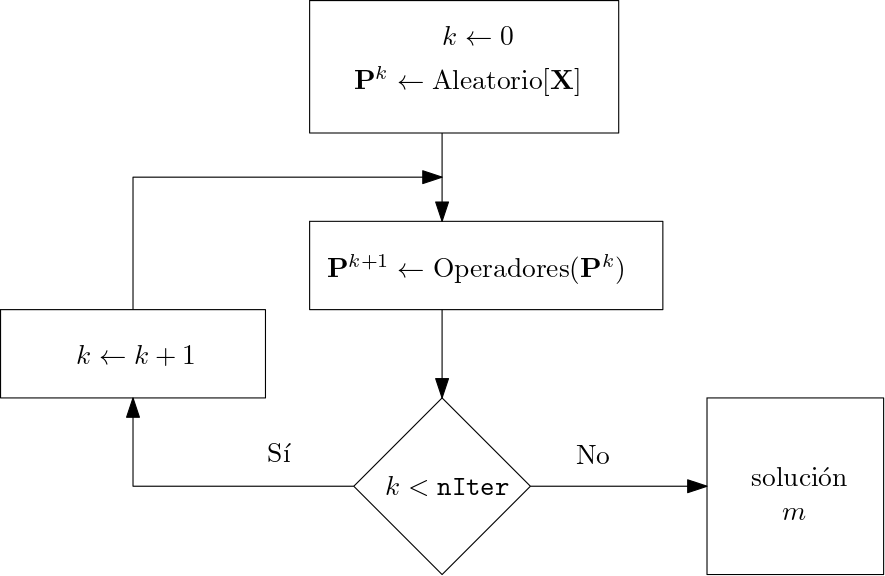
\includegraphics[width=0.7\textwidth]{img/proceso_opti.png}
    \end{center}
    \caption{Proceso de optimización.}
    \label{fig:proceso_opti}
\end{figure} 
 
\section{Algoritmos genéticos} \label{Subsec: 3_4}
Los algoritmos genéticos pertenecen a las metaheurísticas evolutivas que se definieron en la subsección \ref{Subsubsec: 3_3_2}.
%\begin{figure}[H]
%    \begin{center}
%    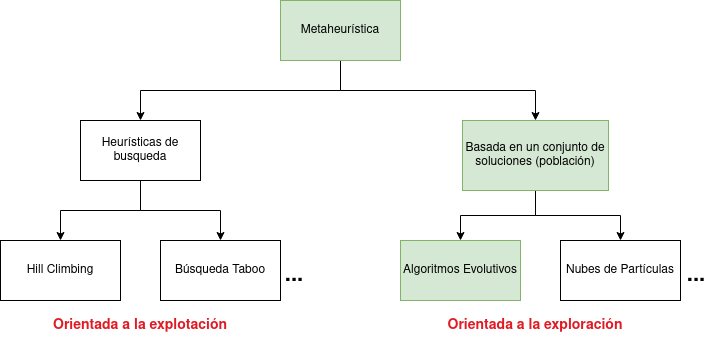
\includegraphics[width=0.8\textwidth]{img/taxo_h.png}
%    \end{center}
%    \caption{Taxonomía de los métodos heurísticos \cite{diaz_lopez_implementation_2023}.}
%    \label{fig:Taxo}
%\end{figure} 
En esta subsección, vamos a profundizar en esta técnica, que será la elegida para la implementación del Capítulo 4.


Los \textsl{algoritmos genéticos}, en adelante GA (del inglés, \textsl{Genetic Algorithms}), son un grupo de algoritmos que se inspiran en la teoría de la selección de la especies de Darwin (1809 - 1882). La selección natural es la base de todo el cambio evolutivo. Es el proceso a través del cuál, los organismos mejor adaptados a su entorno tienen mayor probabilidad de sobrevivir y reproducirse. Esto es debido a la acumulación de las características más positivas en la población a lo largo del tiempo. La información genética de los hijos es heredada de los padres durante el proceso de \textsl{cruce}, aunque en algunos casos es ligeramente modificada debido a algún mecanismo de \textsl{mutación} \cite{e_besada_optimizacion_nodate}.

El artículo en el que John Holland (1929 - 2015) introdujo los Algoritmos Genéticos se titula \textsl{Outline for a logical theory of adaptive systems} \cite{holland_outline_1962}. Fue publicado en 1962 y sentó las bases para el desarrollo de los algoritmos genéticos como una metodología para la optimización y la búsqueda basada en los principios de la evolución biológica y la selección natural. En la Figura \ref{fig:analogia_ga} podemos ver las relaciones conceptuales que estableció Holland. 

\begin{figure}[h]
    \begin{center}
    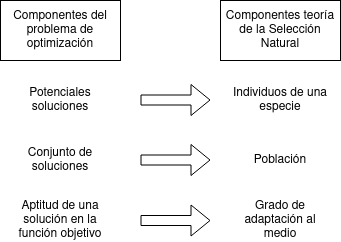
\includegraphics[width=0.5\textwidth]{img/analogia_ga.png}
    \end{center}
    \caption{Relación de conceptos entre la selección natural y los GA.}
    \label{fig:analogia_ga}
\end{figure} 

Partimos de un problema de optimización con restricciones como el de la Definición \ref{COPs}. El GA pretende encontrar la solución óptima de este mediante una serie de funciones que denominados \textsl{operadores genéticos} \cite{yu_introduction_2010}:

\begin{itemize}
	\item \textbf{Selección}: debe permitir que los hijos mejor adaptados tengan, a su vez, mayor descendencia.
	\item \textbf{Cruce}: combina los valores en los genes de los hijos para crear nuevos individuos.
	\item \textbf{Mutación}: modificará a algunos de los hijos de forma aleatoria. 
\end{itemize}

\begin{wrapfigure}{r}{0.5\textwidth}
  \begin{center}
    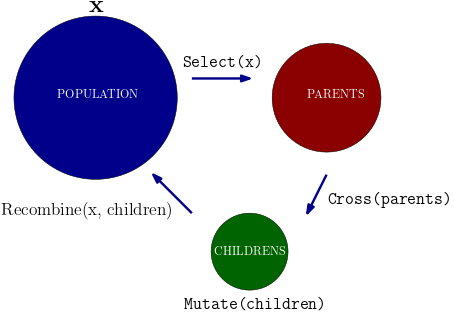
\includegraphics[width=0.48\textwidth]{img/flow_ga.png}
  \end{center}
  \caption{Diagrama de trabajo de un GA.}
  \label{fig:flow_ga}
\end{wrapfigure}

Podemos ver en el Algoritmo \ref{alg: GA_main} el pseudocódigo básico de un GA, y  en la Figura \ref{fig:flow_ga} su diagrama de trabajo, con el que podemos observar cómo se interrelacionan los operadores. En el pseudocódigo encontramos: $x$, que representa a la población (es decir, un conjunto de soluciones del problema) actual, que suele tener un tamaño prefijado y constante a lo largo de la ejecución; por otro lado, $Parents$ representa un conjunto de parejas de individuos seleccionados a partir de la población actual; finalmente, $Children$ serán los nuevos individuos creados a partir del cruce de las parejas de padres. En cuanto a las funciones, tenemos, en primer lugar a $Generate()$, cuya función es dar una población inicial; $Select()$, que elige las parejas de padres, según un cierto método, de entre la población actual $x$; $Cross()$ y $Mutate()$, cruzan y mutan, respectivamente; $Recombine()$ se encargará de, en función de la aptitud de cada individuo, elegir entre las soluciones de la población $x$ y los hijos; finalmente, $Stop()$ tendrá codificada la condición de parada para finalizar el algoritmo. 

\begin{algorithm}[h]
\DontPrintSemicolon
\SetAlgoLined
\SetKwFunction{FGen}{Generate}
\SetKwFunction{FSelect}{Select}
\SetKwFunction{FCross}{Cross}
\SetKwFunction{FMutate}{Mutate}
\SetKwFunction{FRecombine}{Recombine}
\SetKwFunction{FStop}{Stop}
\SetKwProg{Fn}{Function}{:}{}
\SetKwProg{Fn}{Procedure}{:}{}
  \Fn{genetic\_algorithm(Generate, Select, Cross, Mutate, Recombine, Stop)}{
    $x =$ \FGen{}\;
    \Repeat{\FStop{$x$}}{
      $parents =$ \FSelect{$x$}\;
      $children =$ \FCross{$parents$}\;
      $children =$ \FMutate{$children$}\;
      $x =$ \FRecombine{$x, children$}\;
    }
  }
\caption{Pseudocódigo de un GA.}
\label{alg: GA_main}
\end{algorithm}



\chapter{Optimización del Diseño de un Vertipuerto} \label{Capitulo_3}
En este capítulo nos vamos a centrar en la modelización matemática del problema de diseño de un vertipuerto. En primer lugar, se presentan las consideraciones técnicas para el diseño de la infraestructura para, posteriormente, presentar el modelo matemático, así como una explicación detallada de cada una de sus componentes. Las principales fuentes de consulta que han servido para la elaboración del capítulo son \cite{easa_vertiports_2022, federal_aviation_administration_vertiport_2022, park_vertiport_2022}. Además, en este capítulo destacaremos la aportación especial de la entrevista realizada a una de las responsable técnicas del equipo en el que trabajo actualmente en la empresa \textsl{Indra Sistemas S.A}. Esta entrevista puede ser consultada en el Apéndice \ref{app:entrevista}, y nos servirá para comprender mejor cómo se han modelizado las restricciones del modelo matemático.    

\section{Problema de Diseño de un Vertipuerto}
En esta subsección, vamos ver cómo se caracteriza la solución del problema de diseño de un vertipuerto en la línea de trabajos previos relacionados con \cite{park_vertiport_2022}. Además, se darán algunas consideraciones generales del diseño de un vertipuerto, así como la descripción matemática del modelo. 

\subsection{Caracterización de la solución}
Vamos a presentar, a continuación, la formulación matemática del modelo que pretende resolver el problema de 
diseño. En \cite{park_vertiport_2022}, los autores caracterizan el problema a través de una cuadrícula, como se describe en la Figura \ref{fig:cuad_dim_empty}, cuya unidad básica denominaremos \textsl{celda}. Esta puede ser asignada a cualquier infraestructura del vertipuerto (es decir, una celda puede representar una FATO, una puerta de embarque, etc.). Estas celdas son cuadrados de 20 metros de largo, formando una cuadrícula de $8 \times 5$ celdas (las dimensiones de un problema real serán 100 metros de ancho por 160 metros de largo). 

\begin{figure}[h]
    \begin{center}
    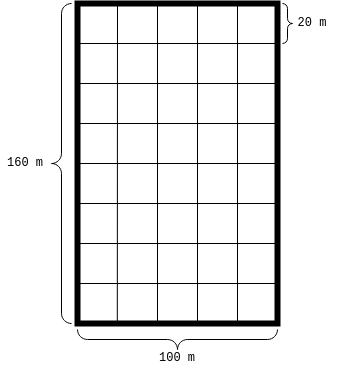
\includegraphics[width=0.5\textwidth]{img/cuad_dim_empty.png}
    \end{center}
    \caption{Caracterización del problema a través de una cuadrícula.}
    \label{fig:cuad_dim_empty}
\end{figure} 

\subsection{Consideraciones del diseño de optimización}
Para definir adecuadamente el modelo matemático, hay que tener en cuenta algunas consideraciones previas en materia de seguridad operacional y desempeño de cada infraestructura. Para ello, los autores de \cite{federal_aviation_administration_vertiport_2022} utilizan el documento \textsl{Draft EB 105, Vertiport Design} del 21 de septiembre de 2022,  elaborado por la FAA (\textsl{Federal Aviation Administration}) de Estados Unidos. Dicho documento también es mencionado por la experta en UTM en la entrevista incluida en el Apéndice \ref{app:entrevista}. En este documento, se proponen las dimensiones de las infraestructuras, así como las \textsl{condiciones de seguridad} y conectividad\footnote{Europa tiene un documento similar llamado \textsl{Vertiports Prototype Technical Specifications for the Design of VFR Vertiports for Operation with Manned VTOL-Capable aeronave Certified in the Enhanced Category}, publicado por la EASA en 2022 \cite{easa_vertiports_2022}.}. En lo sucesivo, CD (o simplemente D), representará la dimensión de control estándar que tomaremos como el diámetro del círculo circunscrito sobre el VTOL en la proyección horizontal del plano, cuando el aparato está en su configuración de despegue o aterrizaje. También se puede definir como la mayor distancia entre dos puntos opuestos de la aeronave (véase la Figura \ref{fig:def_unidad_cd}). 

\begin{figure}[h]
    \begin{center}
    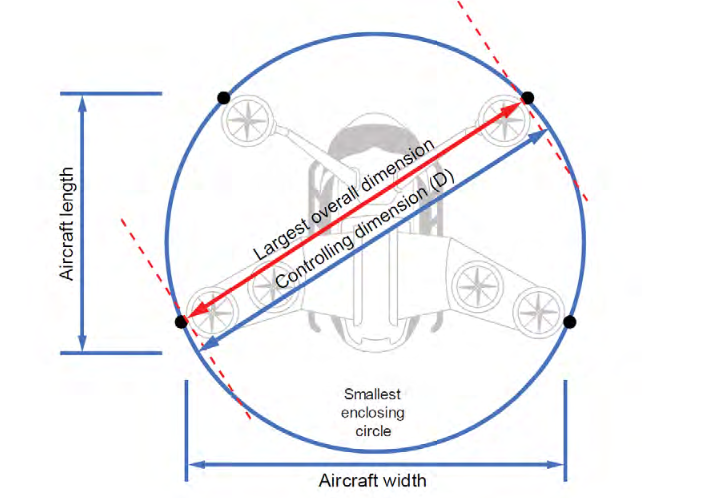
\includegraphics[width=0.5\textwidth]{img/unidad_CD.png}
    \end{center}
    \caption{Dimensión de control \cite{federal_aviation_administration_vertiport_2022}.}
    \label{fig:def_unidad_cd}
\end{figure} 

En base a este concepto, los autores tienen en cuenta los siguientes factores:

\begin{itemize}
			\item El ancho y largo mínimos de una FATO es 2CD unidades de la aeronave de referencia. 
			\item Aunque las dimensiones de las vías y las puertas de embarque no están presentes en \cite{federal_aviation_administration_vertiport_2022}, los autores tomaron como base el documento \textsl{Heliport Design} \cite{administration_heliport_2012}, del cual se infieren las siguientes dimensiones: 
				\begin{itemize}
					\item El ancho mínimo de una vía será 2CD.
					\item El ancho y largo mínimos de una puerta de embarque será 1CD.
					\item La separación mínima entre puertas de embarque será $\frac{1}{3}$CD. 
					\item La terminal de pasajeros es más grande que las puertas de embarque.
				\end{itemize}
		\end{itemize}
En base a esto, las celdas que componen la cuadrícula serán 2CD $\times$ 2CD. 

Respecto a las \textsl{condiciones de seguridad}, los autores las consideran como las más importantes a tener en cuenta, lo cual es coherente con la filosofía del sector. Se tienen en cuenta las siguientes consideraciones: 
	 \begin{itemize}
		\item Los VTOL deben aproximarse al vertipuerto esquivando los edificios que conforman el entorno urbano. Por este motivo, las FATO deben ubicarse teniendo en cuenta las rutas de aterrizaje y despegue. En este estudio, se identifica un conjunto de ubicaciones potenciales para las FATO mediante la evaluación de los obstáculos alrededor del sitio candidato para ubicar el vertipuerto.
		\item Por el propio concepto de UAM, el impacto nocivo que pueda generar un vertipuerto en los alrededores de su ubicación debe ser también un factor tenido en cuenta. En particular, las instalaciones terrestres no deben estar ubicadas alrededor de las rutas de aproximación/salida.
	\end{itemize}

Finalmente, respecto a las condiciones de conectividad, se presentan tanto desde la perspectiva de aeronaves como de pasajeros del UAM. Estas condiciones se dividen en dos: las orientadas al vehículo, que aseguran que las FATO deben estar interconectadas con las puertas, para permitir a las aeronaves dirigirse desde las zonas de embarque hasta las FATO, y viceversa; y las que se centran en los pasajeros, que aseguran que se exijan áreas mínimas para las terminales de pasajeros adyacentes a la puerta de embarque; esto se debe a que los pasajeros sólo pueden acceder a la aeronave por las puertas de embarque. Los autores de \cite{park_vertiport_2022} toman, así, una dimensión equivalente a dos celdas. 


\subsection{Definición del problema de optimización}
El problema de diseño de vertipuertos, que se formaliza a continuación, se presenta formalmente a través de un problema de optimización matemática de programación entera en \ref{eq:f_obj_VDP} a \ref{eq:14_rest_VDP}. Las \textsl{variables de decisión} elegidas $x_{i,j}^{(k)}$ serán binarias. Diremos que es igual a $1$ si la infraestructura $k$ está localizada en la fila $i$ y columna $j$, es decir, la celda $(i,j)$ de la cuadrícula; es igual a $0$ en cualquier otro caso. Tendremos el conjunto de índices 

\begin{equation} 
\mathcal{T} = \{F,G,T,P\}
\label{eq:set_T_infraestructuras}
\end{equation}

donde $F$ son las FATO, $G$ las puertas de embarque, $T$ las calles de rodadura, y $P$ las terminales de pasajeros. Finalmente, el conjunto $\mathcal{C}$ representa todas las celdas de la cuadrícula. Se han elegido estas basándose principalmente en \cite{park_vertiport_2022} y en la entrevista realizada en el Apéndice \ref{app:entrevista}. 

La \textsl{función objetivo} (que se formaliza, a continuación, en \ref{eq:f_obj_VDP}) maximiza el beneficio del operador del vertipuerto, el cual se modeliza fácilmente como la diferencia entre los costes e ingresos totales. Estos se calculan del modo siguiente: 
\begin{itemize}
	\item \textbf{Ingresos}: son calculados como el producto de la \textsl{tasa de uso por avión} ($f$), el \textsl{número de aeronaves} que están usando el vertipuerto (i.e., capacidad del vertipuerto, $v$), y el ciclo de vida de la infraestructura ($l$).  
	\item \textbf{Costes}: el \textsl{coste de construcción} de la infraestructura de tipo $k$ se denota por $c_{\text{con}}^{(k)}$, mientras que el \textsl{coste de operación del vertipuerto por ventana temporal} (\textsl{slot)} es $c_{\text{ops}}$. 
\end{itemize} 

%[RAFA: Esto lo comentamos después, pues el Tribunal puede fijarse en esto como una limitación o que podrías haberlo hecho tu, y no quiero. De momento, déjalo para el trabajo futuro, comentarios en las conclusiones, o algo similar.]
%Los autores señalan que el estudio no tuvo en cuenta la posible tasa por inflación, esto es, el posible impacto que tenga la inflación en las ganancias o rendimiento de los inversores. 
\section{Modelo de optimización}\label{Subsec: 2_2}
Una vez se han definido las componentes principales del modelo matemático, el problema de optimización viene dado por la siguiente formulación matemática:  

\textbf{\textsl{Maximizar}} 
\begin{equation} \label{eq:f_obj_VDP}
f\cdot l \cdot v- \left[ \sum_{k \in \mathcal{T}} c_{\text{con}}^{(k)} \sum_{(i,j) \in \, \mathcal{C}} x_{i,j}^{(k)} + c_{\text{cops}} \cdot l  \right]
\end{equation}


\textbf{\textsl{Sujeto a las restricciones}}
\begin{equation}\label{eq:2_rest_VDP}
v \leq \dfrac{t_{\text{win}}}{t^{(F)}} \sum_{(i,j) \in \, \mathcal{C}} x_{i,j}^{(F)} 
\end{equation}
\begin{equation}\label{eq:3_rest_VDP}
v \leq \dfrac{t_{\text{win}}}{t^{(G)}} \sum_{(i,j) \in \, \mathcal{C}} x_{i,j}^{(G)} 
\end{equation}
\begin{equation}\label{eq:4_rest_VDP}
\sum_{k \in \mathcal{T}} x_{i,j}^{(k)} \leq 1, \quad \forall (i,j) \in \, \mathcal{C}
\end{equation}
\begin{equation}\label{eq:5_rest_VDP}
x_{i-1,j}^{(P)}+x_{i+1,j}^{(P)}+x_{i,j-1}^{(P)}+x_{i,j+1}^{(P)} \geq x_{i,j}^{(G)}, \quad \forall (i,j) \in \, \mathcal{C}
\end{equation}
\begin{equation}\label{eq:6_rest_VDP}
x_{i-1,j}^{(P)}+x_{i+1,j}^{(P)}+x_{i,j-1}^{(P)}+x_{i,j+1}^{(P)} \geq x_{i,j}^{(P)}, \quad \forall (i,j) \in \, \mathcal{C}
\end{equation}
\begin{equation}\label{eq:7_rest_VDP}
x_{i-1,j}^{(T)}+x_{i+1,j}^{(T)}+x_{i,j-1}^{(T)}+x_{i,j+1}^{(T)} \geq x_{i,j}^{(G)}, \quad \forall (i,j) \in \, \mathcal{C}
\end{equation}
\begin{equation}\label{eq:8_rest_VDP}
x_{i-1,j}^{(T)}+x_{i+1,j}^{(T)}+x_{i,j-1}^{(T)}+x_{i,j+1}^{(T)} \geq x_{i,j}^{(F)}, \quad \forall (i,j) \in \, \mathcal{C}
\end{equation}
\begin{equation}\label{eq:9_rest_VDP}
\sum_{k \in \mathcal{T}\setminus \{P\}} (x_{i-1,j}^{(k)}+x_{i+1,j}^{(k)}+x_{i,j-1}^{(k)}+x_{i,j+1}^{(k)}) \geq 2x_{i,j}^{(T)}, \quad \forall (i,j) \in \, \mathcal{C}
\end{equation}
%\begin{equation}\label{eq:10_rest_VDP}
%\text{\textsl{Todas las celdas de taxi están interconectadas.}}
%\end{equation}
\begin{equation}\label{eq:11_rest_VDP}
\sum_{k \in \mathcal{T}} \sum_{(i,j)\in \mathcal{D}} x_{i,j}^{(k)}=0
\end{equation}
\begin{equation}\label{eq:12_rest_VDP}
\sum_{k \in \mathcal{T}\setminus \{T\}} \sum_{(s,t)\in \mathcal{N}(i,j)} x_{st}^{(k)} \leq M \cdot (1-x_{i,j}^{(F)}), \quad \forall (i,j) \in \, \mathcal{C}
\end{equation}
\begin{equation} \label{eq:13_rest_VDP}
\sum_{k \in \mathcal{T}\setminus \{T\}} \sum_{(s,t)\in \mathcal{M} (i,j)} x_{st}^{(k)} \leq M \cdot (1-x_{i,j}^{(F)}), \quad \forall (i,j) \in \, \mathcal{C}
\end{equation}
\begin{equation} \label{eq:14_rest_VDP}
x_{i,j}^{(k)} \in \{0,1\}, \quad \forall (i,j) \in \, \mathcal{C}, \, \forall k \in \mathcal{T}
\end{equation}

%[RAFA: La D es de las celdas Dummy, que aen este momento no han sido explicadas, por lo que el lector puede verse un tanto descolocado, al pensar que es una errata: en lugar de D debería ser C. De momento, lo dejamos así, y ya pensaremos si es necesario aclararlo de algún modo (pie de página, algún comentario antes, etc.).]

donde, los \textsl{parámetros del modelo} que aparecen  en las dos primeras restricciones se definen como sigue

\begin{table}[h]
\centering
\begin{tabular}{|l|l|l|}
\hline
\textbf{Parámetro} & \textbf{Descripción} & \textbf{Unidad} \\ \hline
$t_{\text{win}}$   & ventana de tiempo    & minutos         \\ 
$t^{(F)}$   & separación mínima    & minutos         \\ 
$t^{(G)}$   & cambio de rumbo      & minutos         \\ \hline
\end{tabular}
\caption{Parámetros del modelo.}
\label{tab: cte_1}
\end{table}

\subsubsection{Función objetivo}
En primer lugar, a partir de la Figura\footnote{Esta representación sirve para acompañar la explicación del modelo, por lo que no pretende ser una solución concreta que cumpla las restricciones del modelo.} \ref{fig:ej_rest}, vamos a explicar con mayor profundidad tanto la función objetivo como cada una de las restricciones del problema.

\begin{figure}[h]
    \begin{center}
    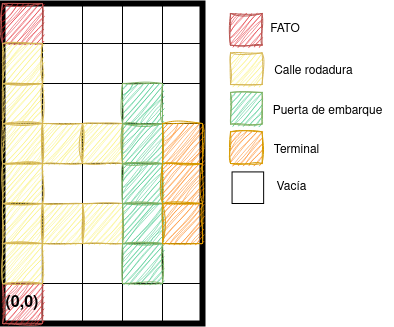
\includegraphics[width=0.5\textwidth]{img/ej_formulas.png}
    \end{center}
    \caption{Representación del diseño del ejemplo.}
    \label{fig:ej_rest}
\end{figure} 

Partimos de la función objetivo (\ref{eq:f_obj_VDP}). Una de las fuentes principales que ayudan a entender la formulación de su definición se extrae de la propia entrevista realizada en el Apéndice \ref{app:entrevista}. Encontramos las constantes $f$, $l$ y $v$, que tomarán los valores de forma acorde a la ubicación y criterios del operador del vertipuerto. A continuación, tenemos la suma del coste de la infraestructura $k$ por aquellas celdas en las que se encuentra ubicada. Finalmente, se suma el producto del coste por ventana de tiempo por el ciclo de vida de la infraestructura. En el desglose del sumatorio, para nuestro ejemplo concreto de la Figura \ref{fig:ej_rest}, y  según el modelo de su infraestructura, se expandiría como sigue:
\begin{itemize}
	\item \textbf{FATO}
		\begin{equation}
			s_{\text{F}} = c_{\text{con}}^{(F)}\cdot \left( x_{00}^{(F)}+ x_{09}^{(F)} \right)
			\label{eq:desglose_ej_f_obj_VDP_FATO}
		\end{equation}
	\item \textbf{Calle de rodadura}
		\begin{equation}
			s_{\text{T}} = c_{\text{con}}^{(T)}\cdot \left( x_{01}^{(T)}+x_{02}^{(T)}+x_{03}^{(T)}+x_{04}^{(T)}+x_{05}^{(T)}+x_{06}^{(T)}+x_{12}^{(T)}+x_{14}^{(T)}+x_{22}^{(T)}+x_{24}^{(T)}     \right) \label{eq:desglose_ej_f_obj_VDP_taxi}
		\end{equation}
	\item \textbf{Puerta de embarque}
		\begin{equation}
			s_{\text{G}} = c_{\text{con}}^{(G)}\cdot \left( x_{41}^{(G)}+ x_{42}^{(G)}+x_{43}^{(G)}+x_{44}^{(G)}+x_{45}^{(G)} \right) \label{eq:desglose_ej_f_obj_VDP_gate}
		\end{equation}
	\item \textbf{Terminales de pasajeros}
		\begin{equation}
			s_{\text{P}} = c_{\text{con}}^{(P)}\cdot \left( x_{52}^{(P)}+x_{53}^{(P)}+x_{44}^{(P)} \right) \label{eq:desglose_ej_f_obj_VDP_P}
		\end{equation}
\end{itemize}
Juntando todos los términos, obtendremos que evaluar la función objetivo corresponde a evaluar la siguiente expresión
\begin{equation}
 f \cdot l \cdot v-(s_{\text{F}}+s_{\text{T}}+s_{\text{G}}+s_{\text{P}} + c_{\text{cops}} \cdot l) 
\end{equation}
\subsubsection{Restricciones}
Las restricciones (\ref{eq:2_rest_VDP}) y (\ref{eq:3_rest_VDP}) limitan la capacidad del vertipuerto en función de las FATO y las puertas de embarque, respectivamente. En estas restricciones encontramos los parámetros de las operaciones del Cuadro \ref{tab: cte_1}. 

Una restricción propia de la caracterización que se ha llevado cabo es la que encontramos en (\ref{eq:4_rest_VDP}), asegurando que cada celda de la cuadrícula no se asignará a más de un tipo de la infraestructura. 

Las restricciones (\ref{eq:5_rest_VDP})-(\ref{eq:9_rest_VDP}) fueron comentadas anteriormente como \textsl{condiciones de conectividad}. Éstas se han divido en dos grupos, de acuerdo a la entrevista realizada en el Apéndice \ref{app:entrevista}: \textsl{condiciones orientadas a los pasajeros}, donde cada puerta debería ser adyacente a una terminal de pasajeros (la terminal de pasajeros debe constar de, al menos, dos celdas), y \textsl{condiciones orientadas a las aeronaves}, en las que se pretende asegurar la interconectividad entre las infraestructuras que conforman el vertipuerto. Las variables de decisión $x_{i,j}^{(k)}$, con $ \; k \in \mathcal{T}$, vimos que determinan si en la celda $(i,j)$ se construye (o no) la infraestructura $k$, que puede ser una FATO, una puerta de embarque, una calle de rodadura, o una terminal de pasajeros. Las restricciones restantes se interpretan del siguiente modo:
\begin{itemize}
	\item \textbf{Restricciones} (\ref{eq:5_rest_VDP}) y (\ref{eq:6_rest_VDP}): si hay una celda de puerta de embarque en $(i,j)$, al menos una de las celdas adyacentes debe ser una celda de pasajero. En la Figura \ref{fig:ej_rest} podemos ver que la restricción se cumple en 
	\begin{equation}
	  x_{22}^{(P)}+x_{42}^{(P)}+x_{31}^{(P)} + x_{33}^{(P)} \geq x_{32}^{(G)} \Rightarrow 0+1+0+0 \geq 1 
	\end{equation}
pero no es así para
	\begin{equation}
	  x_{21}^{(P)}+x_{41}^{(P)}+x_{30}^{(P)} + x_{32}^{(P)} \geq x_{31}^{(G)} \Rightarrow 0+0+0+0 \geq 1 
	\end{equation}
por tanto, observamos que el ejemplo contiene una casilla que no verificaría la restricción (\ref{eq:5_rest_VDP}).
	
	\item \textbf{Restricción} (\ref{eq:7_rest_VDP}): cada puerta debe estar conectada a una calle de rodadura. 
	\item \textbf{Restricción} (\ref{eq:8_rest_VDP}): cada FATO debe estar conectado a una calle de rodadura.
	\item \textbf{Restricción} (\ref{eq:9_rest_VDP}): si hay una celda de terminal de pasajeros en $(i,j)$, al menos dos de las celdas adyacentes pueden ser de cualquier tipo menos de terminal de pasajeros, evitando así callejones sin salida. 
\end{itemize}

Las restricciones que acabamos de comentar suponen un problema para las celdas en los extremos. Por ejemplo, la celda (0,0) no tiene celdas adyacentes ni a su izquierda ni debajo. Para solucionar esta situación, en \cite{park_vertiport_2022} se propone añadir un conjunto de celdas ficticias, denominadas \textsl{dummy}. En la Figura \ref{fig:cuad_dummy}, se observa cómo quedaría la nueva situación al añadir este tipo de celdas, representadas mediante puntos discontinuos. 

\begin{figure}[h]
    \begin{center}
    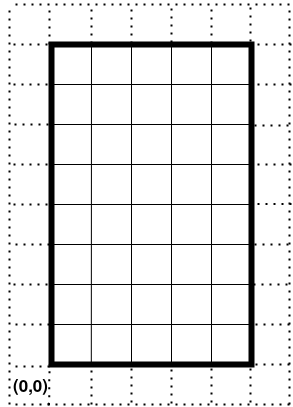
\includegraphics[width=0.4\textwidth]{img/dumy_empty.png}
    \end{center}
    \caption{Celdas \textsl{dummy}.}
    \label{fig:cuad_dummy}
\end{figure} 

El conjunto $\mathcal{D} \subset \mathcal{C}$ estará formado por todas estas celdas \textsl{dummy}. 

Finalmente, las restricciones (\ref{eq:12_rest_VDP}) y (\ref{eq:13_rest_VDP}) utilizan un valor $M$ suficientemente grande para representar términos {\sl big-M}, una técnica usual para este tipo de problemas\footnote{Se puede consultar más información sobre este método en la referencia \cite{cococcioni_big-m_2021}.}. La primera de las restricciones asegura que una FATO en las celdas directamente adyacentes no puede tener infraestructuras críticas (i.e., solo calles de rodadura). Se define el \textsl{conjunto de celdas adyacentes} a la celda $(i,j)$ como
\begin{equation}
\mathcal{N}(i,j) = \{ (i-1,j), \,(i+1,j),\, (i,j-1),\, (i,j+1) \}
\end{equation}
Matemáticamente, se suman todos los tipos de celdas excepto las de tipo $T$ (las calles de rodadura). Si esa celda $(i, j)$ es una FATO, la suma de las celdas adyacentes de tipos no deseados deberá ser $0$. El término $M \cdot (1-x_{i,j}^{(F)})$ es una estrategia matemática habitual para representar la siguiente afirmación: si $x_{i,j}^{(F)}=1$ (es decir, la celda es una FATO), el término \textsl{big-M} se anula, haciendo que la suma pase a ser $0$. Por último, la restricción (\ref{eq:13_rest_VDP}) garantiza que las FATO, puertas de embarque y terminales de pasajeros, no se coloquen en (o cerca de) los caminos de llegada/salida. 



\chapter{Implementación en Python de un GA para el VDP} \label{Capítulo 4}
En este capítulo, vamos a implementar un algoritmo genético que de respuesta al \textsl{Problema de Diseño de un Vertipuerto} (VDP), que presentamos en el Capítulo \ref{Capitulo_3}. En primer lugar, vamos a caracterizar la solución de forma que se adapte adecuadamente al GA, discutiremos su estructura \textsl{genómica}, y daremos detalles de cómo se ha implementado esta en Python. Introduciremos los distintos \textsl{operadores genéticos} que emplean los GA y veremos una forma de calcular la \textsl{aptitud} de los individuos mediante la penalización asociada a las distintas  restricciones del modelo matemático descrito en el Capítulo \ref{Capitulo_3}. Finalmente, veremos dos formas de \textsl{recombinar} las poblaciones, es decir, de como se actualiza la población a través de las generaciones hasta llegar a la función de parada del GA. Las principales fuentes de consulta que han servido para la elaboración del capítulo son  \cite{e_besada_optimizacion_nodate, gestal_pose_introduccion_2023, joines_use_1994, park_vertiport_2022, yu_introduction_2010}.

\section{Algoritmos genéticos para el VDP} \label{Subsubsec: 4_2_1}
En esta subsección, vamos a ver cómo se ha caracterizado la solución, el proceso para implementar los operadores genéticos, cómo se extrae la aptitud de un individuo, y cómo se penaliza dicho valor si el individuo no cumple alguna de las restricciones. Finalmente, veremos diferentes opciones para detener la ejecución del algoritmo diseñado.  
  
\subsection{Caracterización de la solución}

Una de las características diferenciales en los GA es ver como la codificación de las soluciones afecta al tipo de operador\footnote{Durante el resto de capítulo, \textsl{operador} hará referencia a los métodos de \textsl{cruce} y \textsl{mutación}.}. Algunas de las codificaciones más usuales son las siguientes: 

\begin{itemize}
	\item \textbf{Binaria}. En este grupo, las variables de decisión del problema se caracterizan mediante cadenas de \textsl{bits} finitas\footnote{La longitud viene determinada por el tipo de variable de decisión. Por ejemplo, las variables reales con precisión infinita necesitan una cadena binaria de longitud infinita. Como esta no es posible, la longitud de la cadena se determina teniendo en cuenta los valores máximo y mínimo de la
variable real, y la precisión necesaria para representar sus valores \cite{e_besada_optimizacion_nodate}.}.
	\item \textbf{Entera}. Las variables de decisión se representan con cadenas de números enteros. La longitud de la cadena dependerá, de nuevo, del tipo de variable. 
	\item \textbf{Real}. Se utilizan los tipos que brindan los lenguajes de programación (\texttt{float} y \texttt{double}). 
	\item \textbf{Codificación Natural}. En ocasiones, se puede utilizar estructuras de datos directamente ligadas al problema, como grafos o árboles. La elección de una codificación íntimamente relacionada con el problema puede evitar que los operadores de cruce y mutación, que son los responsables de crear y modificar los valores de las posibles soluciones del problema, generen soluciones no factibles \cite{e_besada_optimizacion_nodate}.
\end{itemize}

Es importante destacar que Holland presentó estos métodos pensando únicamente en la representación binaria, ya que ofrece un paralelismo \textsl{ad hoc}, llegando a demostrar de forma teórica su conveniencia frente a otro tipo de representaciones. No obstante, la aplicación práctica, por su parte, ha demostrado que el resto de representaciones son también exitosas. Por ejemplo, en \cite{azketa_algoritmo_2013} utilizan una codificación basada en permutaciones, obteniendo \textsl{soluciones satisfactorias en tiempos
razonables} para un problema de \textsl{despliegue y planificación de sistemas de tiempo real distribuidos}.   

El objetivo de esta sección es definir una codificación adecuada para el problema propuesto en la Subsección \ref{Subsec: 2_2}. Para ello, se ha trabajado con la librería \texttt{numpy}, la cual proporciona la estructura de datos \texttt{array}. Esta estructura cuenta con funciones predefinidas para extraer, manipular y realizar operaciones vectorizadas de forma eficiente.

\begin{figure}[H] 
    	\begin{center}
    	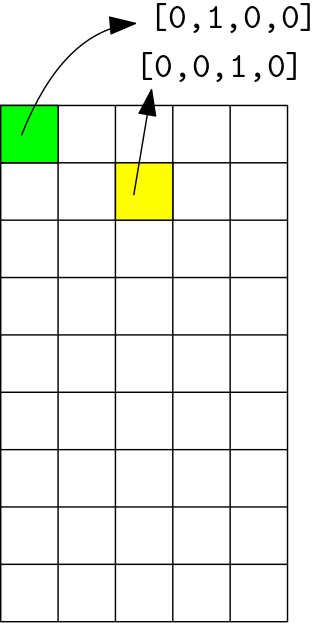
\includegraphics[width=0.2\textwidth]{img/caract_sol.png}
    	\end{center}
    	\caption{Caracterización de la solución.}
    	\label{fig:car_sol}
	\end{figure}

Después de realizar diferentes pruebas, con distintos tipos de caracterización, se decidió tomar una matriz de tres dimensiones: $i$, $j$ y $k$. Particularizando en el problema de diseño de vertipuertos \ref{eq:f_obj_VDP}, partimos de una malla que tendrá $i=1, \ldots, 8$ filas y $j=1, \ldots, 5$ columnas. La tercera dimensión, $k = 1,\ldots, 4$, hará referencia a una lista que contenga cada una de las celdas de la malla. En esa lista estará codificada la información del tipo de infraestructura presente en dicho espacio. Como se puede ver en la Figura \ref{fig:car_sol}, si la celda representa una \textsl{zona de taxi} (utilizando el código de colores presente en la leyenda de la Figura \ref{fig:ej_rest}), la \textsl{lista} estará formada por 0 en las posiciones 0, 1 y 3, mientras que en la posición 2 será un 1. De esta forma, las matrices se definen \textsl{ad hoc} para expresar la información de las variables de decisión $x_{i,j}^{(k)}$ del modelo. En un GA, la codificación de una solución estará compuesta por: 


\begin{itemize}
	\item \textbf{Alelo}: cada valor binario en la posición. Tipos: \textsl{int; binario} $\{1, 0\}$.
	\item \textbf{Gen}: para una celda en una posición dada $(i, j)$. Tipo: \textsl{lista de alelos}.
	\item \textbf{Individuo}: formado por toda la información contenida en la cuadrícula. Tipo: \textsl{array}.   
\end{itemize}


Cabe destacar que no utilizaremos las celdas \textsl{dummy} que se proponen en \cite{park_vertiport_2022}, ya que la propia estructura de datos permitirá recorrerla sin este artificio.  
	
Una vez elegida la forma de codificación de un individuo, podemos definir una función en Python para crear individuos aleatorios. No obstante, siempre que contemos con información que permita centrar la búsqueda, deberemos utilizarla; por ello, vamos a imponer que toda la población inicial cumpla la restricción \ref{eq:4_rest_VDP} del modelo, ya que nos permite generar individuos más aptos de partida. Esto es, obligaremos a que los genes contengan un único tipo de infraestructura. El código completo se encuentra accesible en \cite{gismeros_repositorio_2024}.   

\begin{lstlisting}[language=Python, caption={Función para generar un individuo.}, label={lst:generar_individuo_nuevo}]

def generar_individuo_nuevo():
    """
		Estos individuo ya cumplen la restriccion g_3, es decir, que en una celda hay, a lo sumo, un tipo de infraestructura.
    """
    # Se genera un individuo formado por ceros
    individuo = np.zeros((N_ROW, N_COL, N_INF), dtype=int)
    # Creamos un individuo en 2 dimensiones, siendo 0 -> FATO, 1 -> Gate, 2 -> Taxi, 3 -> Terminal y 4 -> Celda vacia
    elecciones_infraestructura = np.random.randint(
        0, N_INF+1, size=(N_ROW, N_COL))
    # Ahora hay que asignar al array que hay en cada celda un 1 en caso de que tenga una infraestructura de ese tipo
    for tipo_infra in range(4):
        individuo[:, :, tipo_infra] = (
            elecciones_infraestructura == tipo_infra)

    return individuo
\end{lstlisting}

\subsection{Función de generación}
Como ya se ha comentado, su función es construir la población inicial de la que parte el proceso de evolución. Se construye en función del conocimiento que se tiene del espacio de soluciones: 
\begin{itemize}
	\item En caso de que no se disponga de información sobre el valor de las soluciones, la estrategia adecuada será construirlas siguiendo una distribución uniforme sobre los valores de la codificación elegida. La idea es que la población inicial esté compuesta de individuos distribuidos de forma equiprobable sobre el espacio de búsqueda. 
	\item Si se conoce en torno a qué valores se localizan las soluciones, la estrategia sería construir la población inicial siguiendo una distribución Gaussiana entorno a ellos.  
\end{itemize}    

Para facilitar una buena convergencia, hay que evitar que la población converja a un único valor. Se dice que la población inicial debe ser lo suficientemente \textsl{dispersa}. En este sentido, se puede incluir un proceso de generación intermedio que añada algún \textsl{migrante}, esto es, una solución, o conjunto de ellas, que compitan contra los individuos generados por el cruce y mutación, para formar la población de la siguiente iteración. 

En nuestro caso de estudio, para almacenar la información de las diferentes generaciones, utilizaremos los \textsl{DataFrames} de la librería \texttt{Pandas}. Así, la función que genera la población devolverá un \textsl{DataFrame} (véase la Figura \ref{fig:pob_inic}), que contiene las columnas \textsl{id$\_$Individuo}, \textsl{Individuo}, \textsl{Aptitud$\_$Obj} y \textsl{Aptitud$\_$Penalizada}. Las columnas que contienen la información de la aptitud serán tratadas en la Subsección \ref{Subsec: 4_1_3}, cuando se describa la función objetivo del modelo.
 
\begin{lstlisting}[language=Python, caption={Función para crear la población.}, label={lst:crear_pob}]
def creacion_poblacion(tam_pob, c, alfa, beta):
    """
  	Retornamos un DF con: 
  		id_individuo
  		Individuo 
  		Aptitud sin penalizar 
  		Aptitud penalizada
    """
    # Tamano igual al de la poblacinn
    pob = pd.DataFrame(index=range(tam_pob))
	# Asociamos un numero a cada individuo    
    pob['id_Individuo'] = range(0, tam_pob)
	# Generamos un individuo para cada fila    
    pob['Individuo'] = [generar_individuo_nuevo() 
                       for _ in range(len(pob))]
	# Calculamos su aptitud sin penalizar     
    pob['Aptitud_obj'] = pob['Individuo'].apply(fitness)
	# Calculamos su aptitud sin penalizar    
    pob['Aptitud_total'] = pob['Individuo'].apply(
        lambda x: fitness_penalizado_dinamica(x, c, alfa, beta, 1))

    return pob
\end{lstlisting}

En la precondición encontramos, entre los parámetros, el \texttt{tam$\_$pob}, que hace referencia al tamaño de la población, el cual será constante a lo largo de todas las generaciones. El resto de parámetros serán definidos más adelante. 

\subsection{Función de aptitud} \label{Subsec: 4_1_3}
La \textsl{función de aptitud} del problema arroja un valor que mide cómo de \textsl{bueno} es un individuo dado, pero debemos tener en cuenta que existen una serie de restricciones en el modelo. Estas restricciones son las que deben guiar la solución dentro del espacio de búsqueda. La manera habitual de tratar las restricciones en un GA es aplicar una penalización al valor obtenido por el individuo en la función de aptitud.

En \cite{yu_introduction_2010} se define la función que mide si se incumple una restricción como sigue 

\begin{align}
v_j(\mathbf{x}) = \begin{cases}
    ~\max\{0, g_j(\mathbf{x})\} & \text{si } 1 \leq j \leq q \\
    ~\vert h_j(\mathbf{x}) \vert & \text{si } q + 1 \leq j \leq k
\end{cases} \label{eq:incumplimiento_rest}
\end{align}

donde $\mathbf{x}$ será el \textsl{array} que conforma a un individuo. 

Veamos dos ejemplos de cómo definir las funciones $g_j$ a partir de nuestro problema concreto \ref{eq:f_obj_VDP}, ya que, como se comentará más adelante, no tendremos funciones del tipo $h_j$. En primer lugar, la restricción \ref{eq:2_rest_VDP} pasa a ser la función
\begin{equation}
g_1(\mathbf{x}) = v - \dfrac{t_{\text{win}}}{t^{(F)}} \sum_{(i,j) \in \, \mathcal{C}} x_{i,j}^{(F)}
\end{equation}
Para el segundo, tomaremos una de las restricciones del conjunto de condiciones de vecindad; por ejemplo, la \ref{eq:5_rest_VDP} pasa a ser la función
\begin{equation}
g_4(\mathbf{x}) = x_{i,j}^{(G)} - (x_{i-1,j}^{(P)}+x_{i+1,j}^{(P)}+x_{i,j-1}^{(P)}+x_{i,j+1}^{(P)}) , \quad \forall (i,j) \in \, \mathcal{C} \label{eq: ej_4}
\end{equation}
Algunas observaciones:
\begin{itemize}
	\item Dado que la codificación de la solución prescinde de las celdas \textsl{dummy} que se utilizaban en el modelo, la restricción \ref{eq:11_rest_VDP} no formará parte de la implementación, siendo, además, la única función de tipo $h_j$ de las definidas en \ref{eq:incumplimiento_rest}.
	\item Tampoco estará dentro del código la restricción \ref{eq:13_rest_VDP}, dado que solo se pretende ejemplificar el uso de los algoritmos genéticos. Esta restricción hace referencia a un conjunto de celdas que se desprenden de un estudio que los autores de \cite{park_vertiport_2022} hacen sobre las {\sl rutas de aterrizaje y despegue}, en función de posibles obstáculos en la ciudad concreta de Samseong (Seúl).
\end{itemize}

Por tanto, se definen funciones $g_j$, para $j=1,\ldots,9$, que corresponden con las restricciones \ref{eq:2_rest_VDP} - \ref{eq:9_rest_VDP}, y la restricción \ref{eq:12_rest_VDP}, respectivamente. El código de \ref{eq: ej_4} sería la siguiente: 

\begin{lstlisting}[language=Python, caption={Ejemplo de cabecera para una restricción $g_j$.}, label={lst:g_4}]
def g_4(individuo):
    """
    Cada gate debe ser adyacente (arriba, abajo, izq o dr) a una terminal de pasajeros.
    """
    penalizacion_total = 0
    filas, columnas, _ = individuo.shape
    for i in range(1, filas):
        for j in range(1, columnas):
            vecinos = obtener_vecinos(i, j, filas, columnas)
            suma_vecinos = sum(individuo[s, t, 3] for s, t in vecinos)
            if suma_vecinos < individuo[i, j, 1]:
                penalizacion_total += 1
    return max(0, penalizacion_total)
\end{lstlisting} 

A lo largo del proceso de ajuste del algoritmo, se ha añadido una restricción adicional al modelo. Debido al funcionamiento de los algoritmos genéticos y, en especial, el mecanismo de penalización de individuos, que describiremos a continuación, un individuo \textsl{vacío} (aquel que no tiene nada construido) cumple las restricciones del problema y no es penalizado. Para ello, introducimos la restricción \ref{eq:rest_ind_vacio}. 

\begin{equation}
\sum_{(i,j)\in \, \mathcal{C}} \prod_{k \in \mathcal{T}} (1-x_{i,j}^{(k)}) \leq 39   \label{eq:rest_ind_vacio}
\end{equation}
Tomando la numeración de los índices del modelo, no la nativa de Python, para cada celda tendremos un producto de los elementos de la lista, que contendrá cómo se expresa, para $\{x^{(k)}_{1,j} \; \vert\;  j=1, \ldots, 5  \land k \in \mathcal{T} \}$ en \ref{eq:expandir_res_sum}:
\begin{equation}
\left[ 
\prod_{{k \in \mathcal{T}}} (1 - x_{1,1}^{(k)}) +
\prod_{{k \in \mathcal{T}}} (1 - x_{1,2}^{(k)}) + 
\prod_{{k \in \mathcal{T}}} (1 - x_{1,3}^{(k)}) + 
\prod_{{k \in \mathcal{T}}} (1 - x_{1,4}^{(k)}) +
\prod_{{k \in \mathcal{T}}} (1 - x_{1,5}^{(k)})  
\right] + \cdots \label{eq:expandir_res_sum}
\end{equation}
Este producto se anulará siempre que se encuentre una construcción, como podemos ver al expandir $k \in \mathcal{T}$ en la ecuación \ref{eq:expandir_res_prod}:
\begin{equation}
\left[ 
(1 - x_{1,1}^{(1)}) \cdot 
(1 - x_{1,1}^{(2)}) \cdot 
(1 - x_{1,1}^{(3)}) \cdot 
(1 - x_{1,1}^{(4)}) + \ldots \right] \label{eq:expandir_res_prod}
\end{equation}
El valor máximo, es decir, el valor de un individuo \textsl{vacío}, será de 40; por eso, la restricción evalúa si el individuo está por debajo, o en, el valor 39. Para implementarlo, debe ser descrita como una función $g_j$, como puede verse en \ref{eq:g_j_vacias}:

\begin{equation}
g_{10}(\mathbf{x}) = 39 - \sum_{(i,j)\in \, \mathcal{C}} \prod_{k \in \mathcal{T}} (1-x_{i,j}^{(k)})   \label{eq:g_j_vacias}
\end{equation}

Si todas las restricciones son del mismo orden de magnitud, o se han normalizado, el \textsl{incumplimiento total} de las restricciones vendrá dado por cualquiera de las siguientes opciones: 

\begin{equation}
v(\mathbf{x}) = \sum_{j=1}^k \mathbf{\omega_j} \cdot v_j (\mathbf{x}) \quad v(\mathbf{x}) = \max_{j} v_j (\mathbf{x})
\label{eq: violacion_sum_max}
\end{equation} 

donde $\mathbf{\omega_j}$ es un vector de pesos que podemos asociar a las diferentes restricciones en función de su importancia. El valor de aptitud quedará penalizado según
\begin{equation}
f_p(\mathbf{x}) = f(\mathbf{x})+ v(\mathbf{x}) 
 \label{eq:f_pen_general}
\end{equation}

La teoría sobre GA arroja diferentes formas de aplicar \ref{eq:f_pen_general}. Para este trabajo, se ha optado por una penalización \textsl{dinámica}, es decir, un tipo de penalización que permite incrementar los \textsl{parámetros de penalización} de forma correlativa al proceso de evolución. Existen varios esquemas dentro de la penalización dinámica; tomaremos el descrito en \cite{yu_introduction_2010}, propuesto previamente por J. A. Joines y C. R. Houck  en \cite{joines_use_1994}, el cual viene dado por 
   
\begin{equation}
f_p(\mathbf{x}) = f(\mathbf{x})+(c \cdot \mathit{gen})^{\alpha} \cdot v(\mathbf{x})
\end{equation} \label{eq:Joines&Houck}   

cuya función de penalización viene, a su vez, dada por 
 
\begin{equation}
v(\mathbf{x}) = \sum_{j=1}^k v_j^{\beta}(\mathbf{x})
\end{equation}\label{eq:pen_JH}

donde 
\begin{itemize}
	\item $\bm{\alpha} $ es el parámetro que determina el grado de aumento de la penalización a medida que avanza el proceso evolutivo.
	\item $\bm{\beta}$ es el parámetro que influye en cómo se incorpora la penalización en la función de aptitud.
	\item $\mathbf{c}$ es el parámetro que define un factor de escala con el que relacionar la penalización con el número de generaciones ($\mathit{gen}$ en la ecuación).
\end{itemize}

Volviendo a la implementación realizada, tendremos el \textsl{DataFrame} que vimos en la subsección anterior, las columnas \textsl{Aptitud$\_$Obj} que contienen el valor de aptitud calculado según \ref{eq:f_obj_VDP}, y la \textsl{Aptitud$\_$Penalizada} según \ref{eq:Joines&Houck}. Un ejemplo de ejecución arroja el  \textsl{DataFrame} de la Figura \ref{fig:pob_inic}.

\begin{figure}[H] 
    	\begin{center}
    	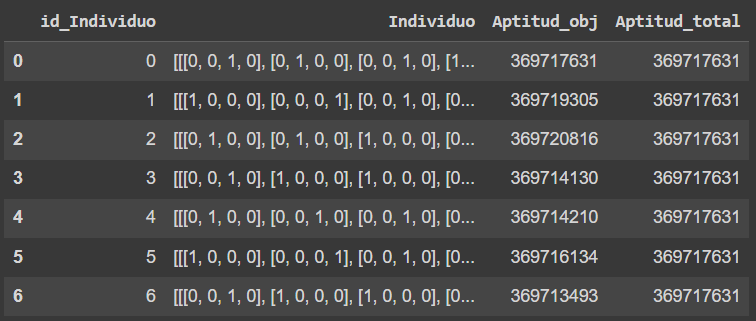
\includegraphics[width=0.7\textwidth]{img/pob_inic.png}
    	\end{center}
    	\caption{Ejemplo \textsl{DataFrame} de la población inicial.}
    	\label{fig:pob_inic}
	\end{figure}

\subsection{Operadores genéticos: Selección}\label{subsec:4_1_4}
Los \textsl{algoritmos de selección} serán los encargados de escoger qué individuos van a disponer de oportunidades de reproducirse y cuáles no \cite{gestal_pose_introduccion_2023}. Como ya se ha comentado anteriormente, los individuos más aptos deben tener una mayor probabilidad de reproducirse, sin embargo, los menos dotados no deben ser eliminados por completo, o la población sería demasiado homogénea, lo que daría lugar al estancamiento en óptimos locales, una convergencia temprana, y a una \textsl{pérdida de información genética}\footnote{Si todos los individuos son iguales, el cruce y la mutación no dará lugar a soluciones innovadoras.}.

En el Algoritmo \ref{alg: f_seleccion} se presenta el funcionamiento general del operador de selección: 

\begin{algorithm}[H]
\DontPrintSemicolon
\SetAlgoLined

\SetKwFunction{FSelect}{Select}
\SetKwFunction{FSelectBasic}{SelectBasic}
\SetKwFunction{FValid}{valid}
\SetKwProg{Fn}{Function}{:}{\Return{$parents$}}

\Fn{f\_seleccion}{
  $parents = \FSelect{x, N\_p}$\;
  \For{$i = 1$ \KwTo $N$}{
    $val(i) = Obj(x(i))$\;
  }
  $i = 1$\;
  \While{$i < N_p$}{
    $parents(i, 1) = \FSelectBasic{x, val}$\;
    $parents(i, 2) = \FSelectBasic{x, val}$\;
    \If{\FValid{$parents(i, :)$}}{
      $i = i + 1$\;
    }
  }
  %\KwRet{$parents$}\;
}
\caption{Algoritmo de selección.}
\label{alg: f_seleccion}
\end{algorithm}

Se eligen $N_p$ parejas de padres de entre las $N$ posibles de la población $x$. En las líneas 1 a 3  del algoritmo, se representa el cálculo de aptitud del individuo en el que profundizaremos en la subsección anterior. Posteriormente, se eligen los dos padres de la pareja, donde $SelectBasic(x, val)$ es un método de selección que debe ser adecuado para el problema en cuestión. Por último, y de forma ``opcional'', dependiendo del método de selección elegido, se verifica si estos padres son una \textsl{pareja válida} (es decir, si no son el mismo padre, o son dos individuos muy similares).


%Encontraremos: 
%
%\begin{itemize}
%	\item \textsl{Métodos estáticos}, donde la probabilidad es constante en toda la generación. 
%	\item \textsl{Métodos dinámicos}, donde la probabilidad depende de cada generación. 
%	\item \textsl{Métodos preservativos}, donde todos los individuos tienen probabilidades de salir elegidos. 
%	\item \textsl{Métodos extintivos}, donde existen algunos individuos con probabilidad nula de ser elegidos. 
%\end{itemize}
%
%La mayoría de métodos se dividen en dos grandes familias: 
%
%\begin{itemize}
%	\item \textsl{Métodos proporcionales}, en los que se tiene en cuenta la contribución de \textsl{aptitud} de cada uno de los individuos con respecto al total de población actual. 
%	
%	La \textsl{aptitud} se calcula según los valores de las funciones de mérito \cite{e_besada_optimizacion_nodate}: 
%	\begin{itemize}
%		\item \textsl{Problemas monoobjetivo}. La aptitud se obtiene directamente de la función objetivo, o bien, está escalada. 
%		\item \textsl{Problemas multiobjetivo}. La aptitud tiene que ser calculada con algún procedimiento que asigne un valor escalar a cada una de las soluciones del problema. 
%	\end{itemize}
%	\item \textsl{Métodos de torneo}, en los que aleatoriamente se toma un subconjunto de soluciones y se extraerá alguna en función de su \textsl{aptitud}.
%\end{itemize}

Los métodos de selección se basan en una probabilidad relacionada con el valor de mérito. De entre los métodos existentes, hemos elegido tres de forma que, posteriormente, podamos comparar resultados. A continuación, vamos a profundizar en ellos. 

En primer lugar, se programa el \textbf{método de la ruleta}. Vamos a ver en qué consiste a partir de la población \ref{fig:pob_inic}:

\begin{enumerate}
			\item Calcular el sumatorio de la aptitud de la población. En este caso, se obtiene 
			\begin{center} 
			$S = $\texttt{ 2588023417}
				 \end{center}	 
			\item Calcular $r$, un número aleatorio, según una distribución uniforme entre $0$ y $S$. En el ejemplo, la ejecución arrojó el valor 
			\begin{center}
			$r = $\texttt{ 1844855395.3541374}
			\end{center}
			
			\item Recorrer la población sumando su aptitud, hasta que la suma sea igual o mayor que $r$:
			
			\begin{figure}[H] 
    	\begin{center}
    	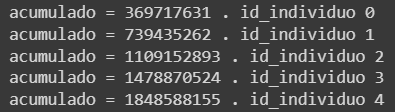
\includegraphics[width=0.7\textwidth]{img/ruleta.png}
    	\end{center}
    	\caption{Proceso para encontrar el individuo cuya aptitud es mayor que $r$.}
    	\label{fig:ruleta}
	\end{figure}
			
			
			\item El primer individuo que supera el valor de $r$ es elegido como padre. En este caso, se corresponde con el índice 4. 
\end{enumerate}
Luego, calculado el primero de los padres, y repitiendo este proceso, encontraríamos el segundo. Se implementan también: 

\begin{itemize}
\item \textbf{Métodos de torneo}. En estos casos se eligen los padres en dos etapas:
	\begin{enumerate}
		\item Primero, hay que tomar un subconjunto (sin tener en cuenta la aptitud de los individuos) de tamaño $T$ de entre todos los de la población actual. 
		\item Después, uno de los individuos del subconjunto será elegido, teniendo en cuenta los valores en la función de mérito. Podemos diferenciar: 
			\begin{itemize}
				\item \textbf{Torneo determinístico}. Entre los individuos del subconjunto se elige el más óptimo. Cuanto más grande es $T$, mayor es la presión de selección de los individuos mejores. 
				\item \textbf{Torneo probabilístico}. En este caso, hay una etapa intermedia en la que, con probabilidad $p >$ 0.5, se determina si el individuo elegido es el más apto o el menos apto del subconjunto. Cuanto menor es el valor de $p$, mayor es la presión de selección de los individuos mejores. 
			\end{itemize}					
	\end{enumerate}		
\end{itemize} 

Han quedado, por tanto, implementados estos tres métodos: ruleta, torneo determinístico y torneo probabilístico, para poder hacer pruebas y ver si existen diferencias significativas en cuanto a los resultados que arroja el algoritmo genético, dependiendo de cuál use como método de selección. 


\subsection{Operadores genéticos: Cruce}
Seleccionados los dos padres, los algoritmos de cruce operan de dos formas diferentes, de acuerdo con \cite{gestal_pose_introduccion_2023}. Se puede optar por una estrategia \textsl{destructiva}, en la que los descendientes pasan a formar parte de la nueva población, sin comparar con el mérito de sus padres. Por contra, una estrategia \textsl{no destructiva} supone que la descendencia pasará a la siguiente generación, si supera el mérito de sus padres. Ambas estrategias pretenden que aquello que hace \textsl{bueno} a un padre se trasmita a los hijos. %si bien puede parecer que las estrategias destructivas pueden dar lugar a descendencias peores que los padres, de alguna manera los genes de estos siguen en sus hijos y puede permitir una búsqueda más diversa y, por tanto, llegar a zonas innovadoras del espacio de búsqueda en la dirección adecuada (que marcan los genes de padres mejores).  

Existen diferentes algoritmos para este operador, pero nos centramos en el que se ha implementado en nuestro código, el \textbf{cruce uniforme}. Se determina, de forma aleatoria y a partir de una probabilidad $p$, si cada alelo está o no en el hijo 1. En caso de que no esté en el hijo 1, estará en el hijo 2.  

		\begin{figure}[h]
    	\begin{center}
    	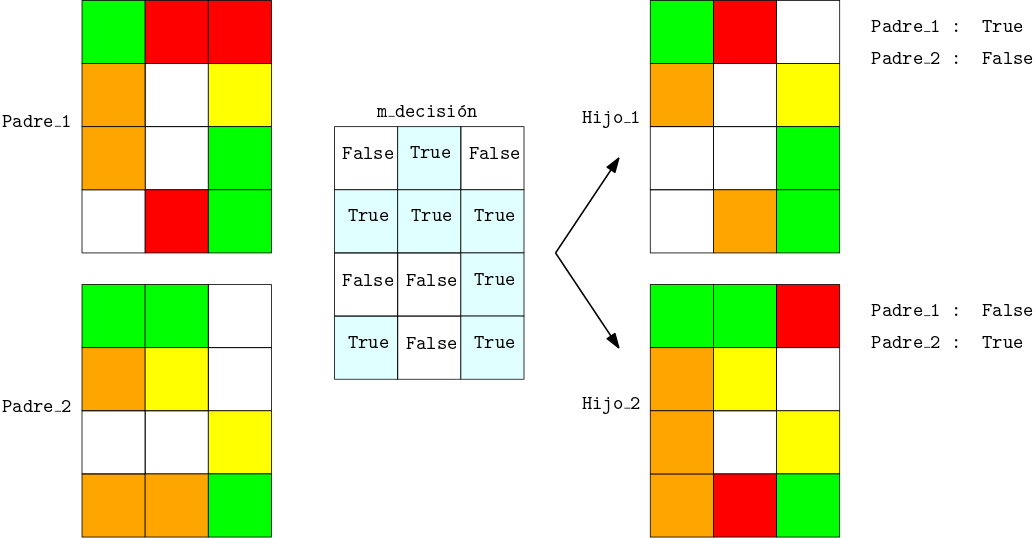
\includegraphics[width=0.75\textwidth]{img/cruce_ejemplo.png}
    	\end{center}
    	\caption{Ejemplo de cruce uniforme según se ha definido en la implementación.}
    	\label{fig:cruce_uniforme}
	\end{figure} 

%	\begin{itemize}
%		\item \textbf{Cruce por $N$ punto}. Se determinan de forma aleatoria $N$ puntos en la cadena a partir de los cuales se crean dos $N+1$ en cada padre. Los hijos tendrán genes de ambos padres mezclados en el orden en que estos aparecían en sus padres. Esta situación se ilustra, para $N=1$ punto, en la Figura \ref{fig:cruce_1_punto}. 
%		
%	\begin{figure}[H]
%    	\begin{center}
%    	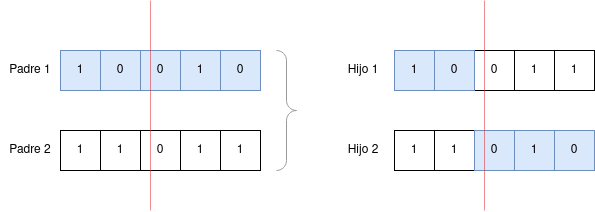
\includegraphics[width=0.8\textwidth]{img/cruce_1_punto.png}
%    	\end{center}
%    	\caption{Ejemplo genérico de cruce por 1 punto.}
%    	\label{fig:cruce_1_punto}
%	\end{figure} 			
%	
%		\item \textbf{Cruce uniforme}. Se determina de forma aleatoria, a partir de una probabilidad $p$, si cada alelo está o no en el hijo 1. En caso de que no esté en el hijo 1, estará en el 2. 
%
%		\begin{figure}[h]
%    	\begin{center}
%    	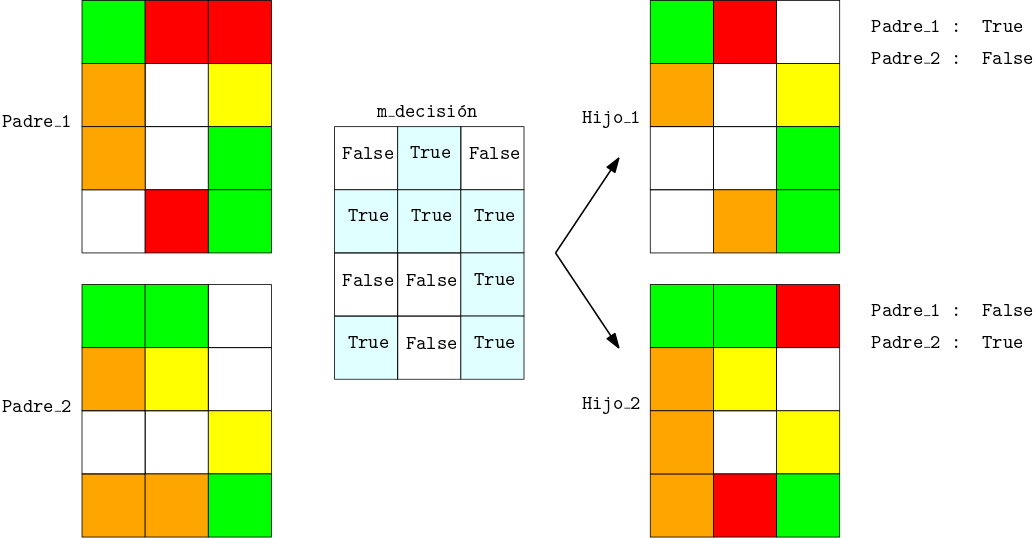
\includegraphics[width=0.75\textwidth]{img/cruce_ejemplo.png}
%    	\end{center}
%    	\caption{Ejemplo de cruce uniforme según se ha definido en la implementación.}
%    	\label{fig:cruce_uniforme}
%	\end{figure} 			
%\end{itemize}

%El esquema elegido para la implementación es el cruce uniforme. 
En la Figura \ref{fig:cruce_uniforme} vemos el comportamiento de este operador a partir de dos individuos, \texttt{Padre\_1} y \texttt{Padre\_2}, y de una \textsl{matriz de decisión}, \texttt{m\_decisión}, del mismo tamaño que un individuo. El contenido de la matriz se calcula según una distribución uniforme, siendo \texttt{True} si el valor es menor que el porcentaje de cruzamiento:
\begin{itemize}
	\item Si \texttt{m\_decisión} es \texttt{True} en la celda $(i, j)$, entonces \texttt{Hijo\_1} tendrá el mismo alelo que \texttt{Padre\_1} en la celda $(i,j)$. 
	\item Si \texttt{m\_decisión} es \texttt{False} en $(i,j)$, entonces \texttt{Hijo\_1} debe completarse con el alelo de la celda $(i,j)$ del \texttt{Padre\_2}. 
\end{itemize}
Para obtener el \texttt{Hijo\_2}, se procede a la inversa. 

La elección del algoritmo de cruce uniforme, como operador de selección en nuestro algoritmo genético, se fundamenta en su capacidad para modular la alteración de patrones a través del parámetro configurable $p$. 

%Véase la Figura \ref{fig:cruce_uniforme}.
%
%Existen métodos específicos para el resto de tipos de representación como: \textsl{Position-based Crossover} para permutaciones o \textsl{Simulated Binary Crossing} para representaciones reales. 
%
%Cuando se decide qué tipo de cruce utilizar en un algoritmo genético, es importante considerar que las características de cada tipo pueden tener un impacto en la manera en que el algoritmo converge. Por ejemplo, el cruce por un punto tiende a preservar en la estructura de los padres, lo que facilita la retención de los patrones existentes en la población actual. Por otro lado, los cruces por varios puntos tienden a romper los patrones con mayor facilidad, por lo que se recomienda no utilizar valores de $N$ altos. Además, en el cruce uniforme, la ruptura de patrones depende de la probabilidad $p$; cuando $p = 0.5$, la ruptura es alta, y a medida que tiende hacia los extremos de sus valores, la ruptura disminuye.

\subsection{Operadores genéticos: Mutación}
La \textsl{mutación} de un individuo supone la transformación de alguno de sus genes, es decir, algunas de las partes de ese individuo se verán afectados por una alteración. Este operador puede actuar en solitario, o ser parte del operador de cruce. En nuestro caso será independiente, es decir, una vez que toda la descendencia ha sido creada, se elige un conjunto de estos para ser candidatos a mutar, en función de una cierta probabilidad $p_m$. A pesar de tener un carácter secundario dentro del algoritmo, es un proceso importante para añadir \textsl{diversidad} y, así, alcanzar regiones distintas del espacio de búsqueda. 

Podemos subdividir el proceso en dos etapas \cite{e_besada_optimizacion_nodate}: 

	\begin{enumerate}
		\item Se calculan las posiciones que serán mutadas utilizando una función aleatoria que determina, en función de $p_m$, si tiene que ser mutado o no.
		\item Se calculan los nuevos valores para los elementos que mutan. En el caso binario se toma el valor contrario.  
	\end{enumerate}

Veamos como funciona este operador en nuestra implementación. Partimos de un individuo de la población de hijos y la {matriz de decisión} \texttt{m\_i}, del mismo tamaño que un individuo. El contenido de la matriz se calcula según una distribución uniforme, siendo \texttt{True} si el valor es menor que el porcentaje de mutación. Si \texttt{m\_i} es \texttt{True} en la celda $(i,j)$, entonces el individuo propuesto para mutar deberá cambiar su alelo de la celda $(i,j)$ (véase la Figura \ref{fig:mutacion_ej}). La creación del nuevo alelo se hará a partir de una función que devuelva una lista con 4 elementos binarios, donde solo uno de ellos será un 1.  

	\begin{figure}[H] 
    	\begin{center}
    	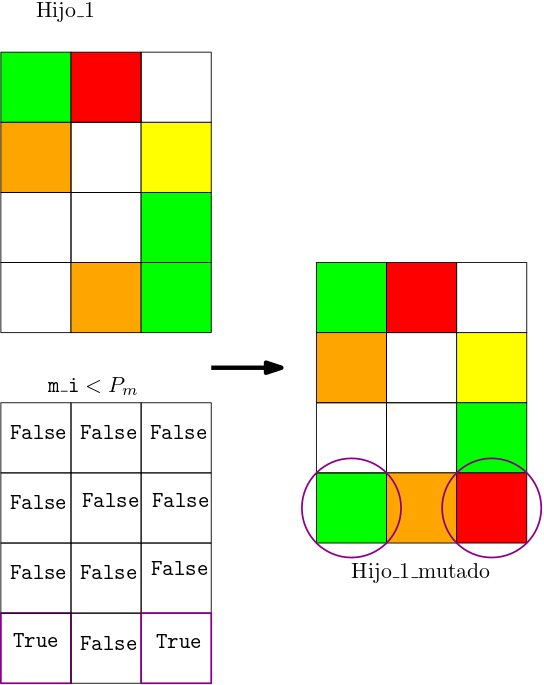
\includegraphics[width=0.5\textwidth]{img/ej_mutacion.png}
    	\end{center}
    	\caption{Ejemplo de proceso de mutación de un individuo.}
    	\label{fig:mutacion_ej}
	\end{figure}

%Dependiendo de la representación existen formas de actuar específicas: \textsl{mutación basada en polinomios}, \textsl{mutación por inserción} o \textsl{mutación por intercambio recíproco} \cite{moujahid_tema_2008}. 

\subsection{Función de recombinación}
La \textsl{función de recombinación} se encarga de, una vez que los operadores de cruce y mutación han generado los nuevos individuos de la población, reorganizarlos para crear la población que pasa a la siguiente generación. Por tanto, necesitamos tomar decisiones sobre cuáles de los individuos antiguos (o nuevos) formarán parte de la población en la próxima generación. Para ellos existen una gran cantidad de métodos, según las diferentes situaciones que se pueden dar. En nuestro caso, hemos implementado la de \textbf{sustitución generacional}.

Entenderemos por \textsl{nueva población} a la formada por los hijos obtenidos del operador de cruce, y que, posteriormente, han podido sufrir una mutación. La \textsl{sustitución generacional} consiste en reemplazar, directamente, la población actual por la nueva. Para mantener constante el tamaño de la población, es necesario crear tantos nuevos individuos como tamaño tenga la población. Esta estrategia puede llevar a perder la mejor solución encontrada hasta el momento; para evitar esta pérdida, la mejor solución obtenida a lo largo de todas las generaciones la hemos guardado en una estructura auxiliar.

Se ha elegido este tipo de recombinación por simplicidad en la implementación. 
%De forma general tenemos: 
%
%\begin{itemize}
%	\item \textbf{Sustitución generacional}: implica reemplazar directamente la población actual por la nueva. Para mantener constante el tamaño de la población, es necesario crear tantos nuevos individuos como individuos existen en la población actual. Esta estrategia puede llevar a perder la mejor solución encontrada hasta el momento. Para evitar esta pérdida, la mejor solución obtenida a lo largo de todas las generaciones puede ser guardada en una estructura auxiliar.
%	
%	\item \textbf{Elitismo}: con el objetivo de asegurar que la población conserve la mejor solución encontrada se puede forzar que esta mejor solución (o un conjunto de ellas) forme parte de la población en la próxima generación.
%\end{itemize}
%
%En nuestra implementación, la estrategia elegida es la de sustitución generacional. 

%Nuestro problema también puede ser tratado como un \textsl{problemas multiobjetivo}. Para estos casos, se pueden utilizar estrategias similares mediante frentes de Pareto, teniendo en cuenta algunas consideraciones adicionales como no variar el tamaño de la población o limitar el tamaño de las estructuras auxiliares. No obstante, existen métodos específicos como el \textsl{NSGA-II} que se considera estándar para problemas multiobjetivo, aunque existen otros métodos que obtienen buenos resultados para problemas concretos como el \textsl{NSGA-III} \cite{yannibelli_comparative_2020}, o el \textsl{MOEA/D} \cite{saglican_moead_2023}. No obstante, finalmente quedo fuera del alcance de nuestra implementación.      

\subsection{Función de parada}
Para que el algoritmo pueda parar de generar las distintas generaciones, es necesario definir una \textsl{condición de parada}. Las versiones más habituales son: 

\begin{itemize}
	\item \textbf{Límite de generaciones}. Se establece un parámetro que limita el número total de generaciones; una vez se alcanza este límite, el algoritmo termina, independientemente de la calidad de las soluciones. 
	\item \textbf{Convergencia poblacional}. El algoritmo también puede terminar cuando la diferencia de los valores de la cadena, o de las funciones de mérito de la población, es menor que un valor prefijado; o bien cuando las mejores soluciones, o sus funciones de mérito, no cambian de forma significativa durante un número prefijado de generaciones \cite{e_besada_optimizacion_nodate}. 
\end{itemize}

En nuestra implementación, se ha elegido la limitación generacional, ya que su puesta en marcha no requiere de ningún ajuste adicional. 

  
%\subsubsection{Otras estrategias poblacionales: Temporal y Copia}
%Durante todo el capítulo hemos supuesto que la población actual está \textsl{congelada} y la recombinación se encarga de crear la nueva a partir de ella, del conjunto de los hijos, y del de los hijos mutados. A esta estrategia se le conoce como \cite{gestal_pose_introduccion_2023} de \textsl{reemplazo de padres}. Existen más tipo de reemplazo. Reemplazo \textsl{aleatorio}, cuando el nuevo individuo se inserta de forma arbitraria; reemplazo de \textsl{similares}, se toma un grupo de individuos de la población actual con un mérito parecido y se reemplaza aleatoriamente los que sean necesarios; reemplazo de \textsl{peores}, de entre los peores se elige aleatoriamente uno que dejará espacio a la descendencia.
%
%Otra estrategia sería la de tener una población \textsl{temporal}. Esta población se inicia vacía y crece a medida que avanza el algoritmo. Para decidir si entran los padres o los hijos se hace en función de una probabilidad $p_c$ que activaría el proceso de cruce y mutación por lo que acabarían entrando los hijos, en caso contraria se añadiría a los padres.  
%
%La \textsl{copia} representa otra estrategia de reproducción utilizada para generar una nueva generación a partir de la anterior. A diferencia del \textsl{cruce}, esta estrategia se enfoca en la reproducción asexual, donde simplemente se duplica un individuo en la nueva generación.
%
%El porcentaje de duplicaciones de una generación a la siguiente se mantiene relativamente bajo, ya que un alto índice de copias podría resultar en una convergencia prematura de la población hacia ese individuo en particular. Esto podría llevar a una notable reducción en el tamaño de la población y limitar la exploración del espacio de búsqueda a un entorno del individuo.
%
%Por lo general, se eligen dos individuos para el cruce, y si este evento finalmente no se lleva a cabo, se incorporan los individuos seleccionados en la siguiente generación.

 
%		\subsection{Algoritmo de optimización de enjambre de partículas} \label{Subsubsec: 4_2_2}
%	\section{Comparativa de rendimiento} \label{Subsec: 4_3}
%		\subsection{Comparativa con trabajos publicados} \label{Subsubsec: 4_3_1}
%	\section{Parámetros de configuración para los algoritmos} \label{Subsec: 4_4}
%		\subsection{Test de similitud de Kruskal-Wallis} \label{Subsubsec: 4_4_1}
%

\chapter{Resultados y Análisis} \label{Capítulo 5}
En este capítulo presentamos brevemente los resultados obtenidos por el algoritmo genético implementado en el Capítulo \ref{Capítulo 4} para realizar un análisis de la sensibilidad de los parámetros que configuran el algoritmo. La principal fuente de consulta que han servido para la elaboración del capítulo es \cite{ugarte2008probability}.
   
\section{Datos del caso práctico} \label{Subsec: 5_1}
Para poner en práctica el algoritmo tomaremos los datos que presentan los autores de \cite{park_vertiport_2022} para un problema de diseño de vertipuertos particular. Los datos concretos se pueden consultar en \ref{tab: valores_cte_PDV}.


\begin{table}[h]
    \centering
    \begin{tabular}{l l l l}
        \hline
        \textbf{Parámetro} & \textbf{Descripción} & \textbf{Valor} & \textbf{Unidad} \\
        \hline
        $l$ & Ciclo de vida de la infraestructura & 10 & Años \\
        $t_{\text{win}}$ & Ventana de tiempo & 60 & Minutos \\
        $t_F$ & Tiempo de retorno de una FATO & 77 & Minutos \\
        $t_G$ & Tiempo de retorno en el vertipuerto & 10 & Minutos \\
        $f$ & Tasa por uso del vertipuerto & 55 & Dólares por aeronave \\
        $c_{\text{con}}(F)$ & Coste de construcción FATO & 77 & Dólares por m\textsuperscript{2} \\
        $c_{\text{con}}(G)$ & Coste de construcción puerta de embarque & 2284 & Dólares por m\textsuperscript{2} \\
        $c_{\text{con}}(T)$ & Coste de construcción celda de taxi & 77 & Dolares por m\textsuperscript{2} \\
        $c_{\text{con}}(P)$ & Coste de construcción terminal de pasajeros & 2284 & Dolares por m\textsuperscript{2} \\
        $c_{\text{ops}}$ & Coste operacional & 1563379 & Dolares por año \\
        $N_{\text{row}}$ & Número de filas & 8 & - \\
        $N_{\text{col}}$ & Número de columnas & 5 & - \\
        $CD$ & Dimensión de control de una aeronave & 10 & Metros \\
        $V$ & Capacidad de aeronaves por hora & 80 & Aeronaves por hora \\
        \hline
    \end{tabular}
    \caption{Datos del caso práctico.}
    \label{tab: valores_cte_PDV}
\end{table} 

\section{Resultados} \label{Subsec: 5_2}
Para la realización de este trabajo, exceptuando la subsección \ref{Subsec: 5_3}, se ha contado con un ordenador portátil con las siguientes características técnicas: 
\begin{itemize}
	\item Marca y modelo de la CPU: Intel Core i5-8250U 1,60GHz.
	\item Memoria RAM: 8 GB DDR4.
	\item Almacenamiento: SSD 512 GB.
	\item S.O. y distribución: Linux, Ubuntu 22.04.3 LTS.
\end{itemize}

%Durante la implementación y ejecución de nuestro algoritmo genético, hemos observado que las soluciones tienden a converger prematuramente hacia un conjunto limitado de soluciones. 

\begin{wrapfigure}{l}{0.5\textwidth}
  \begin{center}
    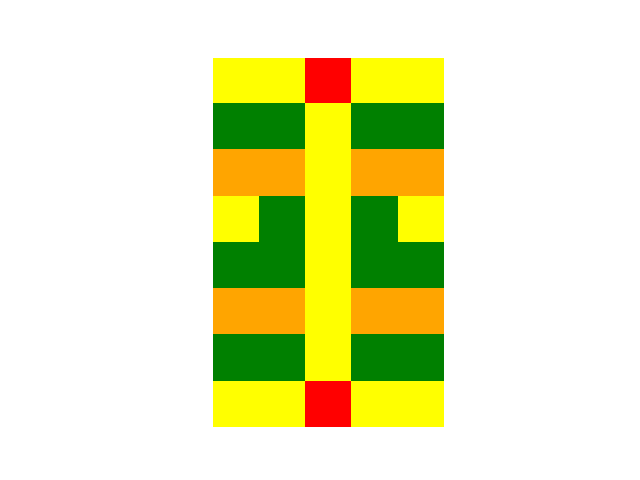
\includegraphics[width=0.4\textwidth]{img/solu_autores.png}
  \end{center}
  \caption{Solución final hallada en \cite{park_vertiport_2022}.}
  \label{fig:sol_autores}
\end{wrapfigure}   

Los valores de aptitud de nuestras soluciones están cercanos a los de la solución propuesta en \cite{park_vertiport_2022}. No obstante, no siempre obtenemos soluciones dentro del rango factible. Este desafío es habitual para este tipo de técnicas, y es la conclusión a la que se ha llegado en la subsección de análisis de sensibilidad \ref{Subsec: 5_4} de este trabajo. 

La solución, definitiva, propuesta por los autores podemos verla en la Figura \ref{fig:sol_autores}. Dicha solución arroja un valor de aptitud de 369754576. 

%	\begin{figure}[h] 
%    	\begin{center}
%    	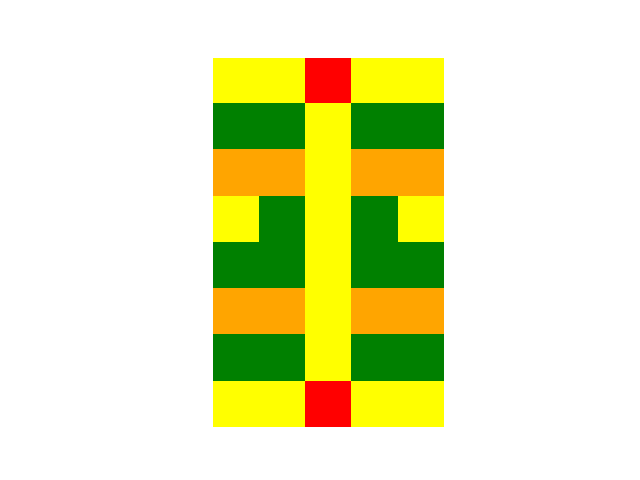
\includegraphics[width=0.3\textwidth]{img/solu_autores.png}
%    	\end{center}
%    	\caption{Solución final hallada en \cite{park_vertiport_2022}.}
%    	\label{fig:sol_autores}
%	\end{figure}

%\begin{wrapfigure}{r}{0.5\textwidth}
%  \begin{center}
%    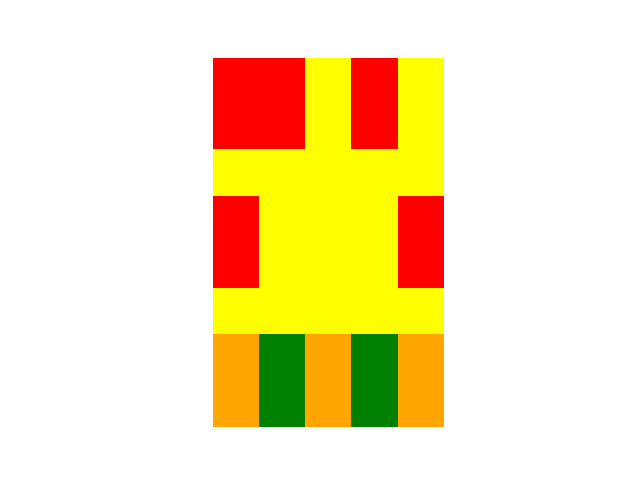
\includegraphics[width=0.4\textwidth]{img/sol_mejor.png}
%  \end{center}
%  \caption{Mejor solución.}
%  \label{fig:sol_mejor_mia}
%\end{wrapfigure}

Por nuestra parte, la mejor solución obtenida la podemos ver en la Figura \ref{fig:sol_mia}. Esta solución, con un valor de 369781060, mejora la aptitud en un 0.007 \% a la mejor solución obtenida por los autores de \cite{park_vertiport_2022}. No obstante, incumple: 
\begin{itemize}
	\item \texttt{g\_6} ya que dos de las puertas de embarque no son adyacentes a una celda de \textsl{taxi}.
	\item  \texttt{g\_7} ya que la celda $(0,0)$ no es adyacente a una celda de taxi y, además, queda rodeada por otras FATO, por lo que también incumple \texttt{g\_9}. 
\end{itemize}

\begin{figure}[h] 
    	\begin{center}
    	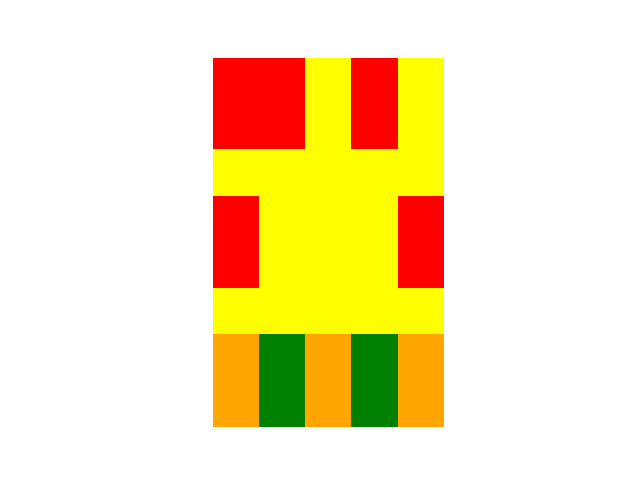
\includegraphics[width=0.41\textwidth]{img/sol_mejor.png}
    	\end{center}
    	\caption{Mejor solución.}
    	\label{fig:sol_mia}
	\end{figure}

Tomando 10 ejecuciones de nuestro algoritmo, la media de aptitud obtenida es 369760415.2, lo cual supone un desvío del 0.001 \% respecto del valor de aptitud obtenido por los autores del artículo. No obstante, mediante la Figura \ref{fig:verti1}, en la que se presentan 2 de las 10 soluciones obtenidas, podemos constatar que no siempre entran dentro de la región de factibilidad. En la Tabla \ref{tab: resumen} se presenta un resumen de los tiempos y aptitudes de la batería de ejecuciones. En dicha tabla encontramos valores de aptitud muy próximos, por lo que la convergencia del algoritmo hacia un óptimo queda puesta de manifiesto, pese a que este no siempre sea factible. Por tanto, lo más probable es que estemos ante una convergencia prematura, lo que nos podría indicar que el algoritmo se ha estancado en un máximo local.

\begin{longtable}{lll}
\hline
      &\textbf{ Mej\_Fit}    & \textbf{Tiempo {[}seg{]}} \\ \hline
\endfirsthead
%
\endhead
%
0     & 369761505   & 45.2             \\
1     & 369761505   & 52.0             \\
2     & 369763866   & 58.6             \\
3     & 369761736   & 49.5             \\
4     & 369751505   & 76.2             \\
5     & 369764020   & 56.8             \\
6     & 369761813   & 51.7             \\
7     & 369757245   & 48.2             \\
8     & 369763789   & 47.9             \\
9     & 369757168   & 56.3             \\ \hline
Media & 369760415.2 & 54.31           \\
\caption{Batería de ejecuciones.}
\label{tab: resumen}\\
\end{longtable}

	\begin{figure}[h] 
    	\begin{center}
    	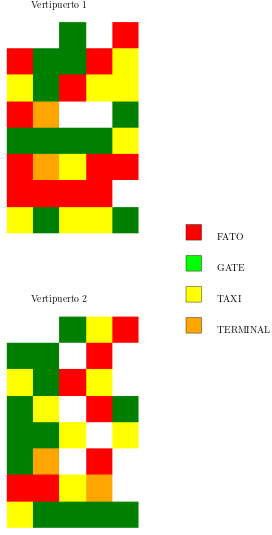
\includegraphics[width=0.4\textwidth]{img/vertis.png}
    	\end{center}
    	\caption{Ejemplos de soluciones.}
    	\label{fig:verti1}
	\end{figure}

De estos resultados, se desprende la necesidad de ajustar correctamente los parámetros del algoritmo genético, de modo que calibremos adecuadamente el comportamiento que tiene éste respecto de las restricciones del modelo. 



\section{Comparación entre algoritmos de selección} \label{Subsec: 5_3}
Como comentamos en la subsección anterior, para las pruebas que hemos realizado en esta subsección, hemos contado con un equipo informático distinto, con prestaciones superiores. Las características técnicas del equipo en cuestión son las siguientes:  
\begin{itemize}
	\item Marca y modelo de la CPU: Intel Core i9-13900H 5.40GHz.
	\item Memoria RAM: 16 GB DDR4.
	\item Almacenamiento: SSD 1 TB.
	\item S.O. y distribución: Windows, 11 Home.
\end{itemize}

En la subsección \ref{subsec:4_1_4}, vimos los tres algoritmos de selección que hemos implementando en el trabajo, estos son: ruleta, torneo probabilístico y torneo determinístico. Como hemos comentado, el equipo informático que hemos utilizado para comparar estos métodos es, significativamente, más potente. Esto se ve reflejado, especialmente, en los tiempos de ejecución.  

Para comparar los algoritmo, hemos creado tres \textsl{DataFrames} con 50 ejecuciones por algoritmo, de modo que, concatenándolos tenemos un \textsl{DataFrame} con 150 observaciones. A partir de este, hemos construido el \textsl{DataFrame} de estadísticas con los atributos: media, mediana y desviación estándar. Gracias al método \texttt{groupby} de la libreria \texttt{pandas}, hemos agrupado los resultados por \textsl{algoritmo de resolución} y calculado cada medida estadística según la mejor aptitud sin penalizar (\texttt{Mej\_Fit}), la mejor aptitud penalizada (\texttt{Mej\_Fit\_Pen}) y el tiempo de ejecución (\texttt{Tiempo\_transcurrido}). 

En primer lugar, si nos fijamos en el gráfico de la Figura \ref{fig:comparar_metodos_1}, las barras de error son relativamente grandes, lo que sugiere una variabilidad considerable en los resultados de cada algoritmo.
El algoritmo de torneo probabilístico tiene el promedio y la mediana más altos, lo que podría indicar un mejor rendimiento en términos de ajuste. Sin embargo, también tiene la mayor variabilidad, como se muestra en la longitud de su barra de error. Finalmente, el algoritmo de ruleta tiene el menor promedio y mediana, y su variabilidad también es grande. El algoritmo de torneo determinístico se sitúa entre los dos en términos de rendimiento y variabilidad.

\begin{figure}[h] 
    	\begin{center}
    	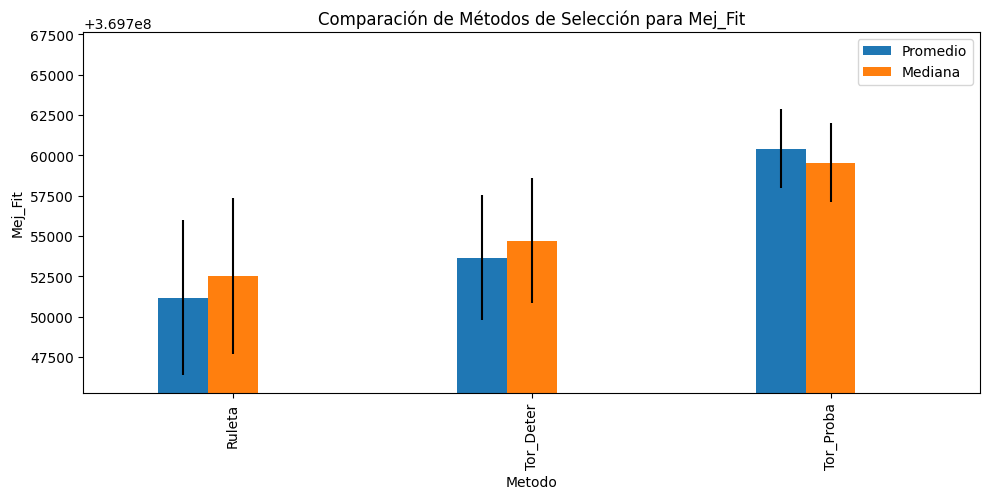
\includegraphics[width=0.7\textwidth]{img/compara_metodos_1.png}
    	\end{center}
    	\caption{Comparación por aptitud sin penalizar.}
    	\label{fig:comparar_metodos_1}
	\end{figure}

A continuación, veamos qué ocurre con la aptitud penalizada. Para ello, observamos la gráfica de la Figura \ref{fig:comparar_metodos_2}. Aquí, la variabilidad es notablemente menor que en la métrica sin penalización de la aptitud. El torneo probabilístico ya no muestra una ventaja clara; de hecho, tiene el promedio más bajo, pero su mediana es competitiva con la del torneo determinístico. El torneo determinístico muestra un mejor promedio que el torneo probabilístico, pero su mediana es más baja que la de la ruleta. Finalmente, la ruleta tiene la mediana más alta, lo que sugiere que cuando se considera la penalización, puede ser un método consistentemente bueno, a pesar de su promedio más bajo.  

\begin{figure}[h] 
    	\begin{center}
    	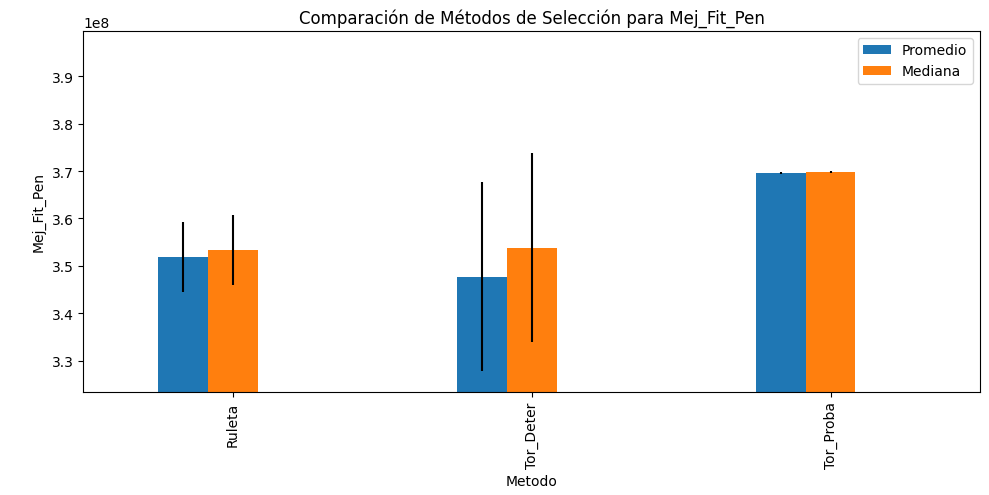
\includegraphics[width=0.7\textwidth]{img/compara_metodos_2.png}
    	\end{center}
    	\caption{Comparación por aptitud penalizada.}
    	\label{fig:comparar_metodos_2}
	\end{figure}

Para terminar, se puede observar en la gráfica de la Figura \ref{fig:comparar_metodos_3}, la variabilidad en el tiempo es menor entre las ejecuciones. El torneo probabilístico tiene el tiempo promedio más bajo y la media más alta, lo que sugiere que es el más rápido pero con variabilidad en los resultados. Finalmente, ruleta y torneo determinístico tienen tienen tiempos promedio más altos que el probabilístico y similares entre sí.      

\begin{figure}[h] 
    	\begin{center}
    	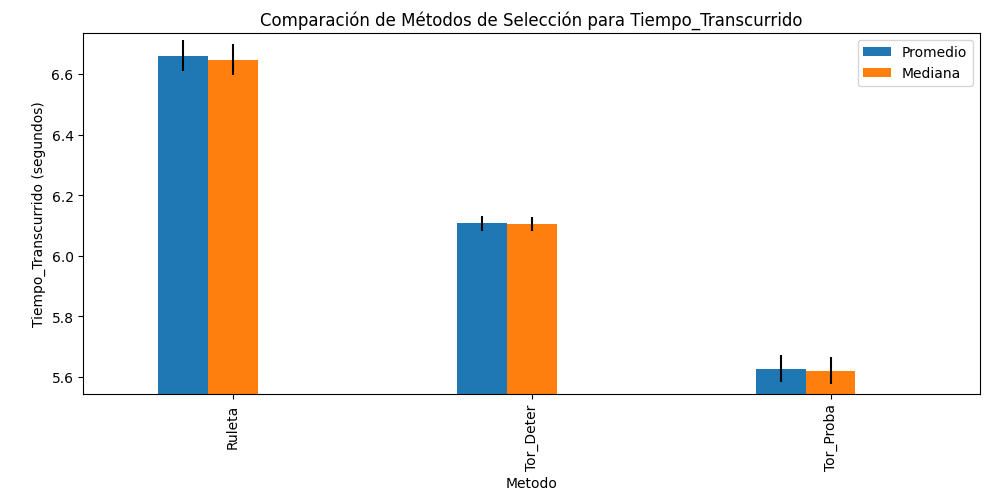
\includegraphics[width=0.7\textwidth]{img/compara_metodos_3.png}
    	\end{center}
    	\caption{Comparación por tiempo de ejecución.}
    	\label{fig:comparar_metodos_3}
	\end{figure}

Estos resultados nos llevaron a tomar la decisión de utilizar el torneo probabilístico para continuar con las pruebas. 

\section{Análisis de Sensibilidad} \label{Subsec: 5_4}
Como hemos visto en la subsección \ref{Subsec: 5_2}, el algoritmo no siempre es capaz de orientar la busqueda de forma que se cumplan las restricciones. Por este motivo, vamos a comenzar por el ajuste de los parámetros de la penalización, de forma que el tratamiento de las restricciones del modelo sea más eficiente. Posteriormente, ajustaremos los parámetros del algoritmo genético. Para ello diseñaremos dos tipos de experimentos, uno en el que compararemos la tendencia de los resultados ajustado el valor de los parámetros $\alpha$ y $\beta$, y otro mediante un modelo de regresión lineal que nos permita llevar a cabo un contraste de hipótesis.  

Dado que vamos a comenzar ajustando los parámetros de penalización, inicialmente, los parámetros del GA los vamos a tomar dentro de unos valores que permitirán, en base a la experiencia con nuestro algoritmo, hacer pruebas en un tiempo razonable de ejecución. Estos valores se pueden consultar con más detalle en la Tabla \ref{tab: par_AG}.

\begin{longtable}[hc]{lll}
\hline
\textbf{}                             & \textbf{Valor} & \textbf{Rango}                              \\ \hline
\endfirsthead
%
\endhead
%
\hline
\endfoot
%
\endlastfoot
%
\textbf{Número de generaciones}       & 500            & $[100, 500]$                                        \\
\textbf{Tamaño poblacional}           & 100            & $[50, 200]$                                         \\
\textbf{Tasa de cruzamiento}          & 0.7            & $[$0.6, 0.8$]$                                        \\
\textbf{Número de parejas}            & 20             & $1 \leq \texttt{tam\_pob} \leq \texttt{tam\_pob}/2$ \\
\textbf{Número de individuos mutados} & 30             & $\lfloor 0.3 \cdot \texttt{tam\_pob} \rceil$        \\
\textbf{Tasa de mutación}             & 0.02           & $[$0.01, 0.05$]$                                      \\ \hline
\caption{Valores de referencia.}
\label{tab: par_AG}\\
\end{longtable} 

\subsubsection{Ajuste de parámetros de penalización}
Los valores teóricos que se proponen en \cite{yu_introduction_2010} para los parámetros de la penalización, que describimos en la subsección \ref{Subsec: 4_1_3}, son: $\alpha = \beta = 2$ y $c = 0.5$. A partir de estos valores, vamos a intentar mejorar la aptitud del mejor individuo de la población para diferentes valores de $\alpha$. Estudiaremos este parámetro en el rango $\alpha \in [1, 5]$ sobre un vector equiespaciado de 20 elementos. Se obtienen los resultados mostrados en la Figura \ref{fig:alpha_analisis1}.

\begin{figure}[h] 
    	\begin{center}
    	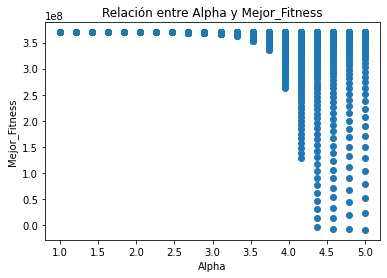
\includegraphics[width=0.6\textwidth]{img/alpha_anl1.png}
    	\end{center}
    	\caption{Valores de aptitud en función del valor de $\alpha$.}
    	\label{fig:alpha_analisis1}
	\end{figure}
 
El gráfico muestra que, para valores bajos de $\alpha$ (cerca de 1.0), la mejor aptitud obtenida tiende a ser relativamente estable y alta. Sin embargo, a medida que el valor de $\alpha$ aumenta, se observa una mayor variabilidad en el mejor valor de aptitud, con muchos valores bajos de aptitud apareciendo, lo que sugiere que un valor de $\alpha$ alto puede no ser favorable para obtener buenos valores de aptitud con este algoritmo genético en particular. Debido a que hay una tendencia clara a partir de 3 hacia valores de aptitud muy pequeños, acotamos el  valor de $\alpha$ hasta 3.25. No obstante, los resultados son parecidos \ref{fig:alpha_analisis2}.

\begin{figure}[h] 
    	\begin{center}
    	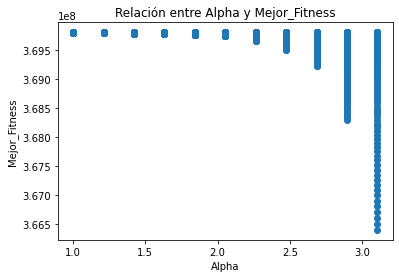
\includegraphics[width=0.6\textwidth]{img/alpha_anl2.png}
    	\end{center}
    	\caption{Valores de aptitud en función del valor de $\alpha$.}
    	\label{fig:alpha_analisis2}
	\end{figure}

Si bien los valores de aptitud son mejores, y están todos en un orden de magnitud parecido, la tendencia continúa apuntado a que los valores óptimos se obtendrán cuando $\alpha$ se aleja de los valores más altos. Tras varias pruebas llegamos al gráfico de la Figura \ref{fig:alpha_analisis4}. 

\begin{figure}[h] 
    	\begin{center}
    	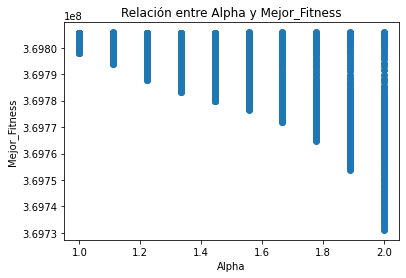
\includegraphics[width=0.5\textwidth]{img/alpha_anl4.png}
    	\end{center}
    	\caption{Valores de aptitud en función del valor de $\alpha$.}
    	\label{fig:alpha_analisis4}
	\end{figure}

Los resultados revelan que el rango de $\alpha$ entre 1.0 y 2.0 mantiene una relación estable con los valores de aptitud obtenidos a lo largo de las generaciones, sugiriendo así una sensibilidad reducida del algoritmo a variaciones dentro de este intervalo. Observamos también que, a pesar de una ligera tendencia hacia la sobrepenalización, el valor de aptitud óptimo se conserva, lo cual implica que la capacidad exploratoria del algoritmo no se ve comprometida con estas configuraciones. En consecuencia, se adoptará un valor de $\alpha$ dentro del intervalo mencionado, aceptando que este rango equilibra adecuadamente la exploración y la viabilidad de las soluciones generadas. Por tanto, tomaremos $\alpha=1.5$.

A continuación, estudiamos la sensibilidad para el valor de $\beta$. Dada la relación que hay entre ambos valores \cite{yu_introduction_2010}, los resultados son similares a la Figura \ref{fig:beta_analisis}, por lo que se decide tomar el mismo valor que para $\alpha$. 

\begin{figure}[h] 
    	\begin{center}
    	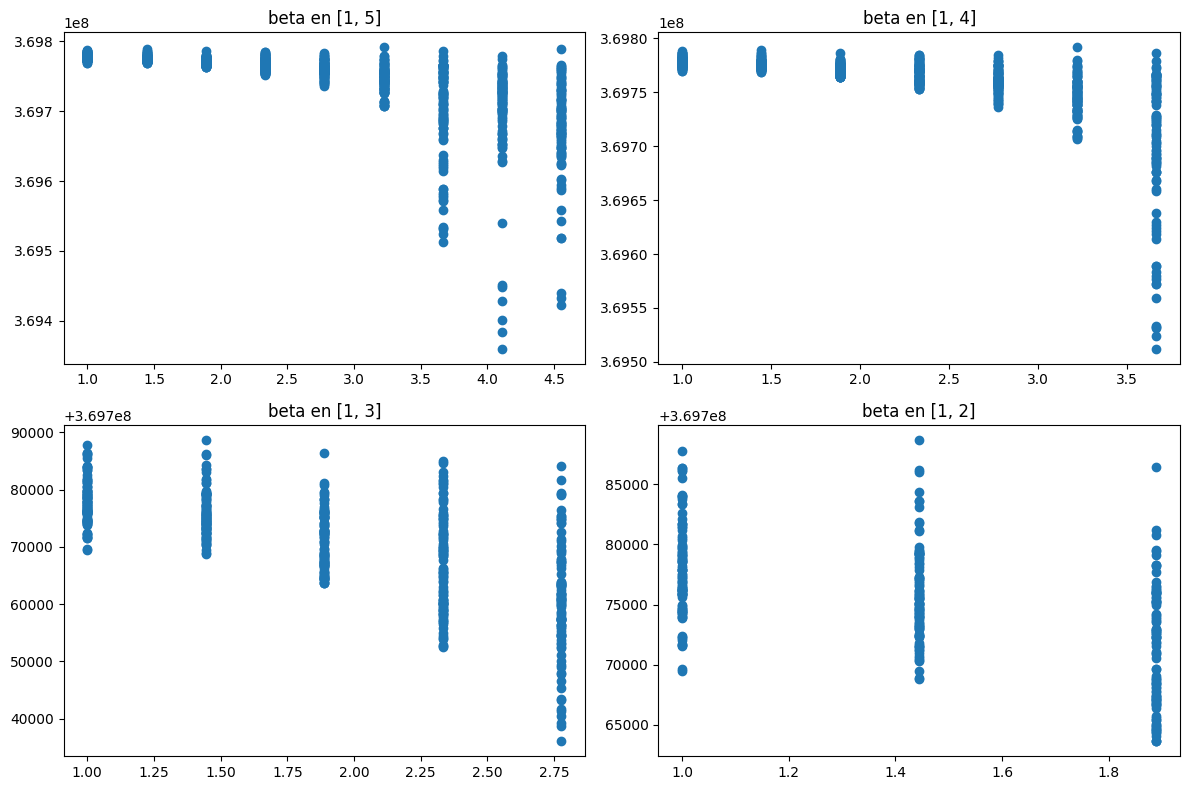
\includegraphics[width=\textwidth]{img/beta_anl.png}
    	\end{center}
    	\caption{Valores de aptitud en función del valor de $\beta$.}
    	\label{fig:beta_analisis}
	\end{figure}

Finalmente, debemos ajustar el valor del parámetro $c$.  Su propósito es actuar como un coeficiente para ajustar la penalización basada en el desempeño de la población actual respecto a las restricciones. Este parámetro ayuda a calibrar el nivel de penalización aplicado en función de cómo la población actual está satisfaciendo las restricciones. Si comparamos el valor de aptitud del individuo que se presenta como mejor solución en \cite{park_vertiport_2022}, el valor 369754576.0, con las aptitudes que maneja el algoritmo, vemos que estamos en el mismo orden de magnitud, e incluso mejorando dicho valor. No obstante, la solución que se presenta en \cite{park_vertiport_2022} es \textsl{más factible}, ya que se comporta mejor respecto de las restricciones del problema. En esta ocasión, vamos a realizar un contraste de hipótesis: 


\begin{equation}
	\left \lbrace \begin{matrix}
		H_0: &\text{Aumentar $c$ no tiene efecto en la factibilidad.} \\
		
		H_1: & \text{Aumentar $c$ mejora la factibilidad.} 
	\end{matrix} \right.
\end{equation}

Tomaremos como métrica, para medir la factibilidad de las soluciones, el número de restricciones violadas, ya que es un buen indicador cuantitativo de la factibilidad de las soluciones. Para ello, definimos dos conjuntos: en el primero de ellos tomaremos un valor de $c$ cercano al recomendado en \cite{yu_introduction_2010}, y en el otro tomaremos un valor ligeramente más agresivo, $c = 1$. Entre la bibliografía específica del Capítulo \ref{Capítulo 4}, encontramos diversos valores utilizados para el parámetro $c$, oscilando entre 0 y 2. En caso de que ir aumentando su valor hasta $c = 1$ sea conveniente, se deberá seguir estudiando, repitiendo este proceso, hasta conseguir ajustar el valor. Finalmente, buscando un equilibrio entre los tiempos de ejecución y el tamaño de la muestra, tomaremos una muestra de 30 ejecuciones por grupo. 

Mediante el \textsl{modelo de regresión lineal simple}, $y = \beta_0 x$, donde $x$ es el valor del parámetro $c$, e $y$ la métrica de la factibilidad, se presentan los resultados obtenidos en las Tablas \ref{tabla:OLS_Results1}, \ref{tabla:OLS_Results2} y \ref{tabla:OLS_Results3}.

\begin{longtable}[c]{l|l|l|l|l}
         & \textbf{coef}   & \textbf{std err} & $t$      & $ P > \vert t \vert $ \\ \hline
\endfirsthead
%
\endhead
%
\textbf{const}    & 2.8879 & 0.242   & 11.930 & 3008272e-17           \\ \hline
\textbf{Valor\_c} & 2.0320 & 0.306   & 6.636  & 1.193014e-08          \\ 
\caption{Coeficientes y $p$-valores del modelo.}
\label{tabla:OLS_Results1}\\
\end{longtable}

En primer lugar, en la Tabla \ref{tabla:OLS_Results1}, vemos que los $p$-valores son menores que 0.05, lo que indica que ambos son estadísticamente significativos.

\begin{longtable}[c]{l|l|l|l|l}

                 & \textbf{R-squared} & \textbf{Adj. R-squared} & \textbf{AIC} & \textbf{BIC} \\ \hline
\endfirsthead
%
\endhead
%
\textbf{Results} & 0.432              & 0.422                   & 109.5        & 113.7        \\ 
\caption{Ajuste del modelo.}
\label{tabla:OLS_Results2}\\
\end{longtable}

En el ajuste del modelo, que podemos ver en la Tabla \ref{tabla:OLS_Results2}, el valor de 0.432 indica que el modelo puede explicar el 43.2\% de la variabilidad de la variable dependiente \texttt{N\_Res\_Violadas}. Dado que no es un valor alto, podría estar indicando que hay más variables que no se han tenido en cuenta, y tienen impacto en el valor que estamos estudiando. De cara a comparar con otros modelos de regresión, sería interesante apuntar los valores obtenidos de los \textsl{criterios bayesiano y de Aikaike} para comparar y poder observar qué otras variables pueden ayudar a explicar mejor el modelo.

\begin{longtable}[c]{l|l|l|l|l}
                 & \textbf{Durbin-Watso} & \textbf{Jarque-Ber} & \textbf{Prob. JB} & \textbf{Skew} \\ \hline
\endfirsthead
%
\endhead
%
\textbf{Results} & 1.796                 & 4.147               & 0.126             & 0.040         \\ 
\caption{Hipótesis del modelo.}
\label{tabla:OLS_Results3}\\
\end{longtable}

Finalmente, centrándonos en los valores de la Tabla \ref{tabla:OLS_Results3}, respecto a las hipótesis del modelo, podemos ver que el valor de 4.147, con un $p$-valor de 0.126 del \textsl{criterio de Jarque-Bera}, sugiere que no hay suficiente evidencia para rechazar la hipótesis de normalidad de los residuos, ya que este $p$-valor es mayor que el umbral común de 0.05. El valor del \textsl{criterio de Durbin-Watson} está por debajo de 2, por lo que no hay una autocorrelación significativa de los residuos y, esto hace que sea poco probable la heterocedasticidad\footnote{Un modelo de regresión presenta homocedasticidad cuando la varianza de los residuos es constante. Si no tiene esta propiedad diremos que el modelo presenta heterocedasticidad.} del modelo.

De este modo, y en función de los resultados de la Tabla \ref{tabla:OLS_Results1}, vemos que el $p$-valor asociado al valor de $c$ es menor que el nivel de significancia usual, por lo que se rechaza la hipótesis nula $H_0$, y, en consecuencia, aceptamos la hipótesis de cambio, concluyendo que el aumento del parámetro $c$ permite mejora la factibilidad de las soluciones.     

Como ya comentamos, sería conveniente repetir este proceso hasta acotar todo lo posible el valor de $c$. En este caso, nos quedaremos con $c=1$, quedando así cerrado el estudio de los parámetros de penalización.

\subsubsection{Ajustes de los parámetros del GA}
El ajuste efectivo de los parámetros de un algoritmo de optimización se puede abordar de diferentes maneras, como se muestra en \cite{garcia_sarmina_comparativa_2022}. En este caso, optaremos por un enfoque sistemático que permita evaluar y ajustar de manera iterativa el impacto de cada parámetro en el rendimiento del algoritmo. Este proceso se divide en diferentes etapas:
\begin{itemize}
	\item \textbf{Selección Inicial}: comenzamos con una selección inicial de parámetros basada en \cite{garcia_sarmina_comparativa_2022}. De esta forma, podemos entender su impacto aislado en el rendimiento del algoritmo haciendo ajustes individuales. En este sentido, utilizamos los valores predeterminados de la Tabla \ref{tab: par_AG}.
	\item \textbf{Ajuste Secuencial}: es el paso que vamos a introducir en esta subsección. Consiste en ajustar los parámetros de manera secuencial, manteniendo los demás constantes. Este enfoque permite identificar interacciones y dependencias entre parámetros. Es crucial evaluar cómo la modificación de un parámetro afecta al rendimiento en presencia de los ajustes previos, permitiendo así una comprensión más profunda de las dinámicas del sistema.
	\item \textbf{Retroalimentación}: después de una pasada inicial por los parámetros, el proceso de optimización se beneficia de un enfoque iterativo, donde se revisan y ajustan nuevamente los parámetros en función de los resultados obtenidos. Este ciclo de refinamiento se basa en la retroalimentación del rendimiento del algoritmo, donde los ajustes anteriores pueden requerir modificaciones. Este enfoque iterativo asegura un ajuste fino, y una optimización más precisa de los parámetros, pero requiere de un tiempo de trabajo considerable. 
	\item  \textbf{Evaluación}: en cada iteración, se debe evaluar el rendimiento del algoritmo considerando todos los parámetros en conjunto. Esta evaluación integral ayuda a identificar configuraciones óptimas que maximicen el rendimiento global del algoritmo.
\end{itemize}

Actualmente existen \textsl{técnicas de optimización} automatizadas \cite{sundhararajan_comparative_1998}: búsqueda en cuadrícula (\textsl{grid search}), búsqueda aleatoria (\textsl{random search}), o algoritmos evolutivos específicos para la selección de parámetros. Estas técnicas pueden explorar, de manera más eficiente, el espacio de parámetros, y ofrecer retroalimentación valiosa para el ajuste.

Partimos de la creación de un \textsl{DataSet} con 81 observaciones de las variables: 
\begin{itemize}
	\item \texttt{n\_gen}: representa el número de generaciones que tendrá cada ejecución. El rango de valores es un vector equiespaciado entre 40 y 200: \texttt{np.linspace(40, 200, 3, dtype=int)}. 
	\item \texttt{tam\_pob}: representa el tamaño, constante, de la población, para cada ejecución. El rango de valores es un vector equiespaciado entre 50 y 200: \texttt{np.linspace(50, 200, 3, dtype=int)}.
	\item \texttt{tasa\_cruz}: representa el porcentaje de cruzamiento para cada ejecución. El rango de valores es: \texttt{[0.6, 0.7, 0.8]}.
	\item \texttt{tasa\_mut}: representa la tasa de cruzamiento para cada ejecución. El rango de valores es: \texttt{[0.01, 0.03, 0.05]}.
	\item \texttt{mej\_fit\_pen}: representa la aptitud del mejor individuo al final de la ejecución.
\end{itemize} 

Establecemos el número de parejas, y de individuos mutados, de forma dependiente del tamaño de la población: 

\begin{align*}
\texttt{num\_parejas} &= \texttt{tam\_pob // 2}, \\
\texttt{num\_indiv\_mutados} &= \texttt{round(0.3 * tam\_pob)}
\end{align*}

Comenzamos viendo las correlaciones entre variables. Inicialmente observamos que existe una fuerte correlación negativa entre el número de generaciones y la aptitud del individuo final; véase la Figura \ref{fig:correlacion1}. Esto es interesante, ya que se esperaría, con más generaciones, que la aptitud mejorara, a menos que esté influenciada por el sobreajuste o por una convergencia prematura.

\begin{figure}[h] 
    	\begin{center}
    	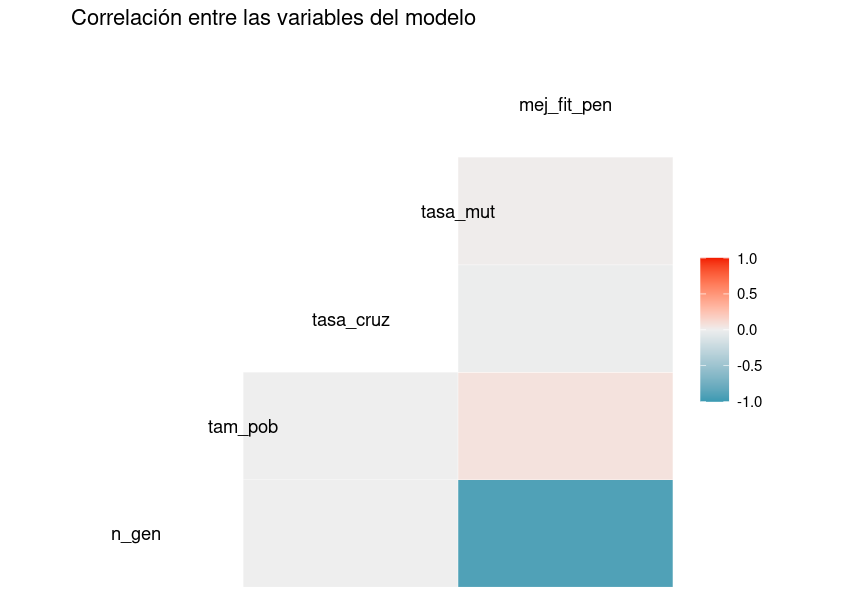
\includegraphics[width=0.6\textwidth]{img/correlacion_grafico.png}
    	\end{center}
    	\caption{Correlación entre \texttt{n\_gen} y \texttt{mej\_fit\_pen}.}
    	\label{fig:correlacion1}
	\end{figure}

Por otro lado, el resto de variables no parece tener un impacto significativo en la aptitud del individuo. 

Fijémonos ahora en la variable aptitud de forma aislada, véase Figura \ref{fig:box_mej_fit_plot}. Observamos que la mediana de la distribución se encuentra cerca del cuartil superior, indicando que más de la mitad de los valores están agrupados hacia el extremo superior del rango. El rango intercuartílico es relativamente corto, lo que sugiere una baja dispersión y, por tanto, una consistencia en los valores de aptitud alrededor de la mediana. No se observan valores atípicos significativos, lo que indica que no hay resultados extremos que distorsionen la distribución. La concentración de los datos sugiere un rendimiento estable del algoritmo en términos de aptitud final, a través de las ejecuciones analizadas. 

\begin{figure}[h] 
    	\begin{center}
    	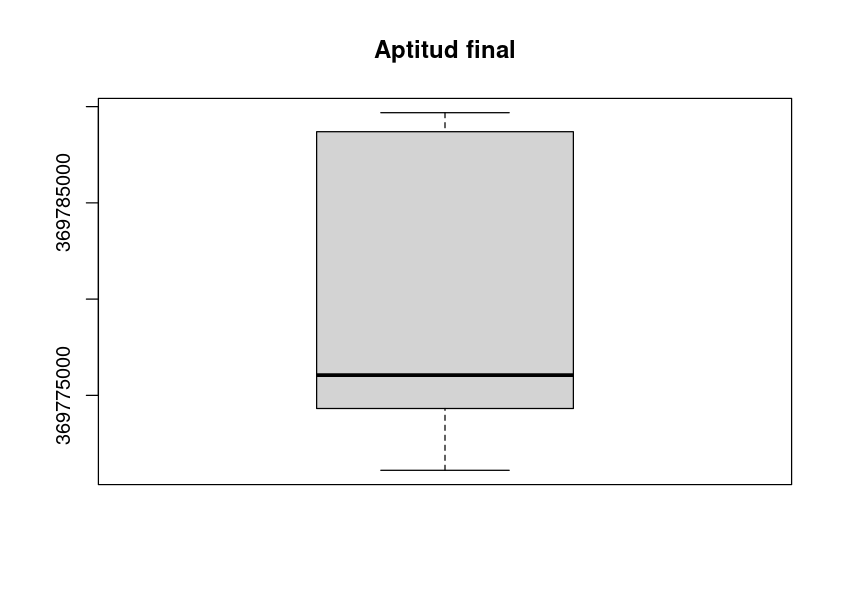
\includegraphics[width=0.5\textwidth]{img/boxplot_mej_fit.png}
    	\end{center}
    	\caption{\textsl{Boxplot} \texttt{mej\_fit\_pen}.}
    	\label{fig:box_mej_fit_plot}
	\end{figure}

Construimos un \textsl{modelo de regresión lineal múltiple}, ya que, a pesar de que la correlación entre variables indica que la única significativa es el número de generaciones, mediante el análisis de varianza (ANOVA) podemos identificar qué variable son estadísticamente significativas. 

\begin{table}[ht]
\centering
\begin{tabular}{lrrrrr}
  \hline
 & \textbf{Df} & \textbf{Sum Sq} & \textbf{Mean Sq} & \textbf{F value} & \textbf{Pr($>$F)} \\ 
  \hline
\textbf{n\_gen} & 1 & 3072041526.90 & 3072041526.90 & 409.53 & 0.0000 \\ 
  \textbf{tam\_pob} & 1 & 17906963.67 & 17906963.67 & 2.39 & 0.1265 \\ 
  \textbf{tasa\_cruz }& 1 & 838109.03 & 838109.03 & 0.11 & 0.7391 \\ 
  \textbf{tasa\_mut} & 1 & 728195.12 & 728195.12 & 0.10 & 0.7562 \\ 
  \textbf{Residuals} & 76 & 570105747.23 & 7501391.41 &  &  \\ 
   \hline

\end{tabular}
\caption{ANOVA modelo completo.}
\label{tabla: modelo_completo}    
\end{table}

En vista de los resultados obtenidos por el el análisis de la varianza, véase la Tabla \ref{tabla: modelo_completo}, con un nivel de significancia del 0.05, observamos que, {\bf tam\_pob}, {\bf tasa\_cruz} y {\bf tasa\_mut} no son estadísticamente significativas en el modelo, es decir, su coeficiente de regresión es nulo. Por tanto, comenzaremos configurando el tamaño de la población. 

Así, el \textsl{modelo de regresión} que vamos a estudiar es $y = \beta_0 x$, donde $x$ es el valor de la variable \texttt{n\_gen}, e $y$ el valor de aptitud \texttt{mej\_fit\_pen}. No obstante, este modelo resulta no cumplir la hipótesis de normalidad en los residuos. Hemos asumido que $\varepsilon_i \sim N(\textbf{0},\sigma^2\textbf{I})$, denominando a este modelo, \textsl{modelo con error normal}. Pero la función de distribución de los residuos que observamos en la Figura \ref{fig:DEN_RES} no sugiere un comportamiento normal. 

\begin{figure}[h]
 	\centering
  	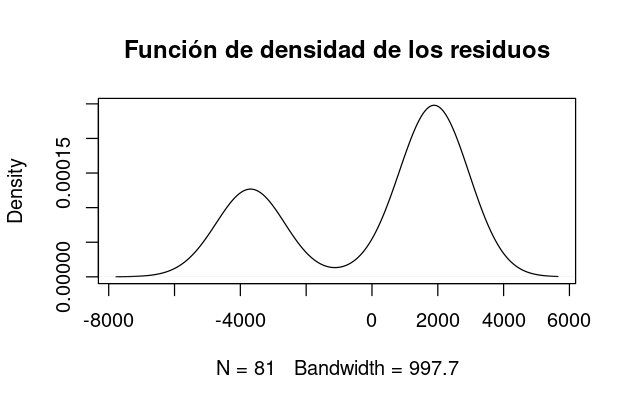
\includegraphics[width=0.5\textwidth]{img/Densidad_residuos.png}
  	\caption{Función de densidad de los residuos.}
  	\label{fig:DEN_RES}
\end{figure}

Por otro lado, si los residuos se distribuyen normalmente, en un gráfico que expresa los cuántiles de los residuos, los puntos en el gráfico deben estar aproximadamente en línea recta. Sin embargo, como vemos en la Figura \ref{fig:QQ_RES}, esto no sucede.  

\begin{figure}[h]
 	\centering
  	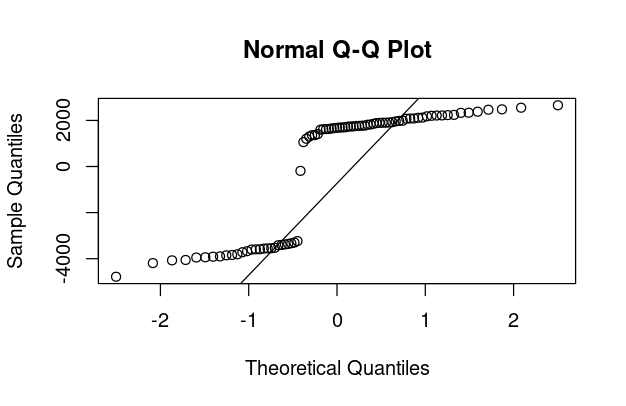
\includegraphics[width=0.5\textwidth]{img/cuantiles_residuos.png}
  	\caption{Normal Q-Q gráfico.}
  	\label{fig:QQ_RES}
\end{figure}

Podemos corroborarlo mediante inferencia con el \textsl{contraste de Safiro-Wilk} \ref{eq: Shapiro-Wilk}.

\begin{equation} \label{eq: Shapiro-Wilk}
\left\lbrace \begin{matrix}
	H_0: & \varepsilon_i \sim N(\textbf{0},\sigma^2\textbf{I}) \\
\\		
	H_1: & \varepsilon_i \not \sim N(\textbf{0},\sigma^2\textbf{I})
\end{matrix} \right.
\end{equation}

\begin{longtable}[c]{lr}
\hline
\multicolumn{2}{c}{\textbf{Test de normalidad}} \\ \hline
\endfirsthead
%
\multicolumn{2}{c}%
{{\bfseries Table \thetable\ continued from previous page}} \\
\hline
\multicolumn{2}{c}{\textbf{Test de normalidad}} \\ \hline
\endhead
%
\hline
\endfoot
%
\endlastfoot
%
\textbf{Prueba}                 & Shapiro-Wilk           \\
\textbf{Datos   }               & residuos               \\
\textbf{Estadístico }          & 0.71961                \\
\textbf{$p$-valor }               & 3.8e-11                 \\ \hline
\caption{Resultados test Shapiro-Wilk.}
\label{tab:testSW}\\
\end{longtable}

El resultado del test de normalidad de Shapiro-Wilk, para los residuos \ref{tab:testSW}, indica que la hipótesis nula, en la que los residuos se distribuyen normalmente, debe ser rechazada, ya que el $p$-valor es prácticamente nulo, por debajo de cualquier nivel de significancia al uso.

Llegados a este punto, una estrategia a seguir consistiría en tomar un valor intermedio de generaciones, y volver a construir un \textsl{DataSet} configurando el resto de parámetros en sus valores más óptimos. 

\begin{figure}[h]
 	\centering
  	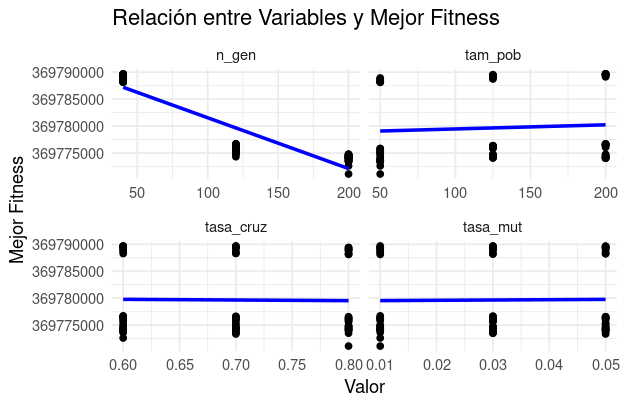
\includegraphics[width=0.7\textwidth]{img/n_gen_vs_fit.png}
  	\caption{Comparación de las variables con la Aptitud.}
  	\label{fig:fit_vs_todos}
\end{figure}

Dado el estudio completo que se ha llevado a cabo en este capítulo, parece haber una convergencia prematura en el algoritmo lo que lleva a que algunas soluciones \textsl{no evolucionen lo suficiente}. Algunas de las estrategias que se podrían seguir son las siguientes: 

\begin{itemize}
	\item \textbf{Selección de individuos diversa}: utilizar algoritmos de selección que favorezcan la diversidad genética en la población. Por ejemplo, \textsl{la selección por torneo} puede modificarse para incrementar la probabilidad de seleccionar individuos menos adaptados.

    \item \textbf{Cruzamiento y mutación adaptativos}: ajustar las tasas de cruzamiento y de mutación dinámicamente durante la ejecución del algoritmo, en función de la diversidad genética de la población. Si la diversidad disminuye, aumentar la tasa de mutación puede ayudar a introducir nueva variabilidad genética en la población.

    \item\textbf{Inserción de nuevos individuos}: periódicamente, introducir nuevos individuos en la población, generados al azar (o mediante otros métodos de optimización), puede ayudar a mantener o aumentar la diversidad genética.

    \item \textbf{Uso de múltiples objetivos}: implementar una función de aptitud que considere múltiples objetivos, en lugar de trabajar con penalizaciones.
\end{itemize}

Estos son sólo algunos de los caminos que se podrían tomar para mejorar esa convergencia prematura detectada y, posteriormente, volver sobre el análisis de los parámetros. 


\chapter{Conclusiones y Trabajo Futuro} \label{Capítulo 6}
En este capítulo final, resumiremos los principales hallazgos de nuestra investigación sobre la aplicación de algoritmos genéticos al problema de diseño óptimo de vertipuertos, destacando las contribuciones más relevantes, y cómo estas permiten avanzar en el conocimiento del campo. Discutiremos también las implicaciones prácticas de nuestro trabajo, junto con las limitaciones encontradas durante el proceso de investigación. En base a estas reflexiones, presentaremos posibles direcciones para un futuro estudio, que puedan abordar las brechas identificadas, explorar nuevas preguntas que surjan durante su desarrollo, y aplicar los conocimientos adquiridos en contextos más amplios o específicos.
\section{Conclusiones} \label{Subsec: 6_1}
Los objetivos que se marcaron al principio de la investigación fueron la profundización en la movilidad aérea urbana y el negocio UTM, enfocándonos en dominar y aplicar heurísticas evolutivas, como los algoritmos genéticos, para mejorar las soluciones existentes en \cite{park_vertiport_2022}. Planeamos mejorar las habilidades de programación en Python aprendidas durante el Grado para implementar estos algoritmos de manera efectiva, buscando soluciones factibles y mejores a problemas del mundo del UTM, basándonos en la optimización heurística. Además, queríamos comparar los resultados obtenidos con nuestra implementación,  para finalmente dedicar esfuerzos en el ajuste de parámetros que permitiera realizar un estudio de sensibilidad, con el fin de incrementar la calidad de las soluciones propuestas.

Los objetivos principales de aprendizaje sobre algoritmos genéticos, negocio UTM e implementación se han cumplido.  El trabajo realizado ha permitido dos cosas, por un lado, entender mejor lo que podía estar fallando en la implementación para futuras mejoras; y por otro, analizar mejor el modelo matemático, así como esbozar pequeños cambios en las restricciones que puedan mejorar considerablemente la implementación. No debe olvidarse que éstas fueron concebidas pensando en métodos de resolución exactos. 

Cabe destacar que el uso de algoritmos genéticos ha supuesto un desafío que, al punto en el que queda esta investigación, aún conllevaría un trabajo importante para poder igualar la calidad de las soluciones que pueden ofrecer métodos exactos tradicionales. Si bien el tiempo de cómputo de estos métodos puede ser elevado, podría verse compensado por el esfuerzo que supone la optimización del modelo matemático, de los parámetros y de la implementación. Y es que, sin lugar a dudas, uno de los fuertes de las heurísticas es el uso de conocimiento experto para el desarrollo del algoritmo. Pero a la vez, considero, lo convierte en una herramienta poco trasversal y escalable a otros problemas, mientras que un \textsl{software} comercial tiene un uso más universal. Si nos fijamos en los valores de aptitud que hemos conseguido no distan mucho de los que ofrecen en \cite{park_vertiport_2022}. Existen numerosos estudios que utilizan los algoritmos genéticos para optimizar la localización geográfica de un vertipuerto \cite{brunelli_new_2023, shin_skyport_2022}, en cambio, las referencias sobre el uso de este tipo de técnicas de optimización para el VPD es más limitado. Por tanto, representa un avance, que aunque modesto, permite ampliar el conocimiento que se posee sobre este. La exploración realizada puede servir de punto de partida para futuros estudios con los que abrir nuevas líneas de investigación, contribuyendo así al desarrollo continuo de este campo de vanguardia.

Finalmente, a nivel personal, el aprendizaje de estas técnicas ha supuesto un reto a nivel teórico y práctico. Desde las primeras lecturas de publicaciones se pudo observar la complejidad que supone modelar un problema real en el ámbito aeroespacial. Respecto a la implementación, si bien Python es un lenguaje ``amigo'', quiero destacar que la imposibilidad de depurar una ejecución debido al gran número generaciones, dentro de las cuales se hacen, a su vez, multitud de operaciones, ha sido un verdadero desafío. Por otro lado, enfrentarme a una implementación que roza las 800 líneas de código ha supuesto un verdadero aprendizaje para un estudiante del Grado de Matemáticas. Principalmente, debido a la complejidad inherente del proyecto, la necesidad de comprender y optimizar cada fragmento del código, así como asegurar la integración efectiva de todas las partes, con el fin de que funcione de forma cohesionada e integrada. 

Esta investigación supone también la culminación de mis estudios en el Grado de Matemáticas y, concretamente, del itinerario de Computación. Los contenidos de este trabajo me han permitido aplicar gran parte de los conocimientos adquiridos en dicho itinerario: estructuras de datos, diseño de algoritmos, recursividad, son sólo algunas de las principales herramientas que se han desplegado a lo largo de este trabajo; pero nada de esto habría sido posible sin la sólida base matemática que he adquirido durante el grueso de mi estudios. Muchas disciplinas matemáticas han formado parte de este trayecto: optimización, análisis multivariable, álgebra y modelos estadísticos, entre otras, son, de nuevo, sólo algunas de ellas. Ha sido muy gratificante poder ``unirlo'' todo; en ocasiones, ``los árboles no nos dejan ver el bosque'', y las matemáticas son un bosque enormemente rico y lleno de matices que, en su conjunto, se convierte en una herramienta poderosa que no tiene límites.

\section{Trabajo futuro} \label{Subsec: 6_2}
En primer lugar, una de las mayores limitaciones que se han presentado a la hora de realizar este trabajo, ha sido el equipo informático. Esto queda de manifiesto en el contraste entre los tiempos de ejecución de las subsecciones \ref{Subsec: 5_2} y \ref{Subsec: 5_3}. Por tanto, las pruebas y ajustes del algoritmo se han visto afectadas. En el futuro, realizar el análisis de sensibilidad completo con un equipo informático con mejores prestaciones puede ayudar a encontrar una configuración para los parámetros más eficiente.  

En este trabajo hay tres pilares que requieren de atención: el estudio de la penalización de las restricciones, la convergencia prematura y la optimización de los parámetros. 

En cuanto a la penalización de las restricciones, existen numerosos métodos, más o menos sofisticados, para abordar este problema \cite{yu_introduction_2010}. Sería conveniente explorar diferentes estrategias, e incluso trabajar en adaptar alguna a la situación concreta del modelo del problema presentado en esta memoria. 

Respecto a la convergencia prematura, se han dado las siguientes vías de investigación: selección de individuos diversa mediante otros métodos de selección, cruzamiento y mutación adaptativos, inserción de nuevos individuos generados al azar o por otros métodos de optimización y, finalmente, el uso de múltiples objetivos como alternativa a la penalización por incumplimiento de las restricciones; véase el Capítulo \ref{Capítulo 5} para una información más detallada.

Finalmente, la optimización de los parámetros podría ser mejorada. Por ejemplo, mediante métodos específicos para algoritmos genéticos, o con técnicas generales más dirigidas, las cuales, además, optimicen el tiempo dedicado a esta parte del proceso. 


Sería también una gran aportación implementar y comparar los resultados obtenidos con diferentes técnicas de optimización como los algoritmos de enjambres de partículas, u otros algoritmos bio-inspirados. Esto no sólo pretende buscar un método algorítmico mejor, si no que también se pueden utilizar sus soluciones como migrantes de las poblaciones del algoritmo genético y, de esta forma, acotar de forma más precisa el espacio de búsqueda.  

Me gustaría, especialmente, tratar en mayor profundidad el problema de optimización de operaciones en un vertipuerto \cite{espejo-diaz_heuristic_2023}. Si bien la infraestructura es vital, en mi puesto de trabajo actual, el principal problema es cómo van a interactuar las aeronaves dentro de ella. En este sentido, creo que puede ser una buena vía de investigación para el futuro. 

Finalmente, las restricciones del modelo pueden ser revisadas con mayor detalle. Los propios autores de \cite{park_vertiport_2022} comentan la idoneidad de buscar nuevas restricciones de colectividad que no se han tenido en cuenta como, por ejemplo, que todas las celdas de taxi estén conectadas.


  
\newpage

\medskip
\nocite{*}
\bibliographystyle{plain}
\bibliography{biblio}
\clearpage

\newpage

\appendix
\chapter{Entrevista previa realizada} \label{app:entrevista}
Durante el desarrollo de esta investigación, tuve la oportunidad de entrevistar a Marta García, responsable técnica del equipo encargado de los proyectos europeos de los que se hace cargo la división de UTM (de sus siglas en inglés, \textsl{Unmanned Traffic Management}), equipo del que formo parte en \textsl{Indra Sistemas} desde mayo del 2023. Marta es Ingeniera Aeroespacial y Máster en Sistemas de Trasporte Aéreo por la Universidad Politécnica de Madrid. Actualmente, ocupa el puesto de Ingeniera Senior de Sistemas U-space\footnote{\textsl{El denominado ``concepto U-space'' engloba un conjunto de sistemas, servicios y procedimientos específicos que han sido diseñados para permitir el acceso seguro, eficiente y asequible al espacio aéreo de operaciones de UAS numerosas o complejas, sobre la base de desarrollos técnicos con un alto grado de digitalización y automatización} \cite{sostenible_concepto_2023}.} y ATM (de sus siglas en inglés, \textsl{Air Traffic Management}) con amplia experiencia en proyectos relacionados con el UTM. La entrevista se llevó a cabo con el objetivo de obtener perspectivas valiosas sobre el diseño de vertipuertos debido al profundo conocimiento que Marta tiene de este tipo de infraestructuras. En concreto, Marta lleva la carga principal del proyecto EUREKA \cite{proyEUREKA}, el cual está destinado a desarrollar los procesos de llegada, salida y cambio de dirección para los vertipuertos. Sus aportaciones han sido útiles no sólo para la elaboración de esta investigación, sino también para mi crecimiento profesional como Ingeniero de Sistemas en Indra. A continuación, se presenta la transcripción completa de la entrevista. 


\begin{itemize}
	%PREGUNTA 1
	\item[\textbf{P}:]\textbf{ ¿Qué factores influyen en el beneficio de un vertipuerto?}
	\item[\textbf{R}:] \textsl{Para poder medir con la máxima veracidad posible el beneficio de un vertipuerto habría que tener en cuenta qué tasa de uso tiene en cuanto a la cantidad de operaciones tanto de carga de mercancías como de pasajeros se consiguen cubrir. Al hilo de esto mismo, dependerá mucho la capacidad del vertipuerto. Si se prepara un vertipuerto que tiene la capacidad suficiente para abarcar la demanda esperada, el beneficio será mucho mayor que si tiene más capacidad que demanda o viceversa. De hecho, otro factor importante es saber que el vertipuerto está construido con vistas a poder servir el tráfico no solo actual, sino también que depara en lo siguientes años. Siempre se pueden llevar a cabo modificaciones en cuanto a futuras demandas, pero el estar preparado para ellas en la medida que se puede, aporta gran beneficio a la infraestructura global.}
	%PREGUNTA 2 
	\item[\textbf{P}:] \textbf{¿Cuáles son las infraestructuras básicas que conforman un vertipuerto?}
	\item[\textbf{R}:] \textsl{Un vertipuerto tiene que constar, como mínimo, de las siguientes infraestructuras:
\begin{itemize}
	\item FATO(s).
    \item Zona de aparcamiento o \textsl{stand(s)}. En algunos casos, podría coincidir la FATO con el \textsl{stand}, pero para un vertipuerto en el que se espera cierta carga de tráfico, esto no sería viable.
	\item Calle de rodaje o taxi, en el caso habitual de que la FATO no coincidiera con el STAND.
	\item Hangar(es) con zona de carga de baterías y donde se podrían incluir oficinas para operadores.
	\item Terminal o zona de espera para pasajeros.
	\item Torre de control o similar para alojar a los operadores del vertipuerto. Al igual que sucede con aviación tripulada, se podría analizar el caso de torres remotas y, en ese caso, incluso poder alojarse junto a controladores de aviación tripulada.
\end{itemize}}
	%PREGUNTA 3
	\item[\textbf{P}:] \textbf{¿Qué factores influyen en el coste de la infraestructura?}
	\item[\textbf{R}:] \textsl{ El coste de la infraestructura estará delimitado por lo siguientes factores:
	\begin{itemize}
		\item El primero de ellos, el coste de planificación. Antes de iniciar los trabajos de edificación, debe existir un estudio que analice la demanda de pasajeros y operaciones, llevando a cabo los respectivos pronósticos, de manera que se pueda tomar una primera decisión sobre la inversión total a realizar.
     \item El segundo, y siguiendo la línea de la pregunta anterior, los costes de construcción y correspondiente mano de obra de las propias infraestructuras.
     \item El tercero y último correspondería a los costes de testeo, validación y certificación del vertipuerto por parte de las autoridades competentes.
	\end{itemize}    }
	%PREGUNTA 4	
	\item[\textbf{P}:] \textbf{¿Cuáles son los principales factores que afectan el rendimiento operativo de un vertipuerto?}
	\item[\textbf{R}:] \textsl{El rendimiento operativo de un vertipuerto puede llegar a estar limitado por múltiples factores, sobre todo cuando se habla del manejo de VTOL como un vehículo que, hasta ahora, no se ha tratado en una infraestructura independiente junto a otros vehículos.
Principalmente se podría decir que los factores de mayor afección son:
	\begin{itemize}
		\item Disponer de una red segura para poder cerciorarse de que los VTOL pueden operar bajo los niveles de seguridad esperados. Esto es, proteger adecuadamente las zonas de rodaje, \textsl{stands}, carga de baterías, FATO, etc. Esto no solo se refiere a disponer estas áreas en zonas libres de obstáculos, sino a señalizarlas correctamente y a que tengan las separaciones adecuadas entre unas y otras para poder evitar potenciales conflictos en las operaciones.
        \item Disponer de suficientes centros de carga. El rendimiento se puede ver enormemente decrementado si un vehículo no puede realizar su carga a tiempo porque no dispone del servicio adecuado.
        \item Se ha de disponer de un servicio de mantenimiento 24 horas de cara a posibles problemas que puedan sufrir los vehículos en cualquier fase de su operación.
        \item Disponer del suficiente personal para operar en el vertipuerto. Esto comprende tanto a los gestores/controladores del mismo, como al \textsl{staff} necesario en FATOS e infraestructuras adyacentes.
        \item Disponer de las ayudas adecuadas de radiovigilancia y navegabilidad, de manera que se puedan gestionar correctamente las operaciones de los VTOL.
	\end{itemize}}
        
	%PREGUNTA 5
	\item[\textbf{P}:] \textbf{¿Cómo se podría medir la eficiencia operativa de un vertipuerto?}
	\item[\textbf{R}:] \textsl{Bajo mi opinión, la eficiencia operativa de un vertipuerto debe tener en cuenta diferentes factores y no consolidarse con un cálculo único en el cual puedan faltar ciertas métricas de elevado interés. Digamos que se trataría de asignar ciertos indicadores operativos que podrían formarse. Por ejemplo:
	\begin{itemize}
		\item Número de operaciones de drones por hora/media hora en términos tanto de despegue como de aterrizaje. El hecho de calcularlo de 30 minutos en 30 minutos radica en el hecho de que estos vehículos tardan mucho menos tiempo en realizar el rodaje, despegue y aterrizaje que las aeronaves tripuladas.
    \item Movimiento diario de pasajeros.
    \item Número de operaciones que se pueden gestionar simultáneamente. En función del tamaño del vertipuerto, varios drones podrían despegar o aterrizar al mismo tiempo (similitud con el caso de las aproximaciones paralelas de aviación tripulada).
	\end{itemize}
	}
	%PREGUNTA 6
	\item[\textbf{P}:] \textbf{¿Cómo se aborda la disposición de las diferentes infraestructuras que conforman el vertipuerto?}
	\item[\textbf{R}:] \textsl{En el momento de abordar la disposición de las infraestructuras, se requiere realizar un estudio previo en el que se pueda analizar la demanda esperada, el tipo de drones que se espera que operen en el vertipuerto, la geografía del lugar y la cercanía a áreas críticas como puede ser un aeropuerto. Además de esto, se debería tener en cuenta la cercanía a áreas urbanas siempre evitando potenciales molestias de ruido, emisiones y/o interferencias con otras infraestructuras ya que la mayor parte de las operaciones esperadas de los VTOL serán de gran utilidad en estas zonas (tanto transporte de pasajeros como de carga).}
	%PREGUNTA 7	
	\item[\textbf{P}:] \textbf{¿Qué factores intervienen a la hora de ubicar las infraestructuras que conforman el vertipuerto?}
	\item[\textbf{R}:] \textsl{Los factores a tener en cuenta en el momento de ubicar las infraestructuras básicas de un vertipuerto se pueden dividir en lo que respecta a, tal y como llamamos en el caso de aeropuerto, lado tierra (afección a pasajeros) y lado aire (afección a vehículos). De esta manera, para el lado aire, los factores que intervienen en esa ubicación serían:
	\begin{itemize}
		\item Las servidumbres de seguridad de la zona.
    \item El espacio aéreo adicional necesario para la fase de aproximación y salida de drones.
    \item La disposición de \textsl{stands} respecto a terminales de pasajeros debe estar correctamente dispuesta de manera que cada una conecte con un \textsl{stand}.
    \item Los \textsl{stands} han de estar conectados de manera adecuada con las zonas de calles de rodaje de VTOL.
    \item De la misma manera, esas calles de rodaje han de estar correctamente conectadas con una o varias FATO.
    \item Las calles de rodaje deberán estar debidamente distanciadas y la conexión entre ellas no debería abarcar ángulos muy pequeños siendo, como mínimo, de 90 grados.
\end{itemize}
Y para el lado tierra:
\begin{itemize}
	\item Las zonas de acceso al vertipuerto deberán estar posicionadas cerca de la terminal de carga de pasajeros para evitar largos trayectos.
    \item Las terminales tendrán que disponer de tantas zonas de embarque como sean necesarias para poder cubrir la demanda esperada.
	\end{itemize}
     }
	%PREGUNTA 8	
	\item[\textbf{P}:] \textbf{¿Existen desafíos particulares o estrategias que se emplean para garantizar tanto la comodidad de los pasajeros como la eficiencia en el movimiento de las aeronaves dentro de las instalaciones?}
	\item[\textbf{R}:] \textsl{Aparte de la ya mencionada guía publicada por la FAA, actualmente cada país está buscando su propia estrategia para tratar de acomodarse tanto a las necesidades de los vehículos como a las de los pasajeros. Se busca con ello tener una aproximación similar a la que se emplea en aeropuertos. Esto es, de cara a los pasajeros:
	\begin{itemize}
		\item Disponer de zonas de descanso en las propias terminales.
    \item Posicionar los vertipuertos en zonas en las que se pueda facilitar un aparcamiento gratuito o de bajo coste.
    \item Distribuir pantallas en la terminal y en el propio VTOL de manera que se pueda visualizar la información relativa a la operación a realizar y que así el pasajero pueda sentirse cómodo.
 \end{itemize}   
Y de cara al movimiento de vehículos:
\begin{itemize}
    \item Evitar que las calles de rodaje se encuentren muy cerca unas de otras.
    \item Evitar ángulos agudos de conexiones entre calles para no tener que realizar grandes giros constantemente en vuelo.
    \item Disponer las FATO, \textsl{stands} y calles de rodaje de manera que la rodadura no sea muy extensa.
    \item Facilitar las zonas de salida de hangares tras la debida carga de los vehículos y que el acceso a las calles de rodaje sea sencillo.
	\end{itemize}}
    
	%PREGUNTA 9	
	\item[\textbf{P}:]\textbf{¿Cómo se aborda la distribución espacial de las áreas críticas para garantizar la seguridad y eficiencia de las operaciones?}
	\item[\textbf{R}:] \textsl{La FAA publicó recientemente la primera guía de diseño y disposición de vertipuertos. Aunque en Europa se está empezando a trabajar en generar algo similar, es una buena pauta a seguir en el momento de conocer cómo abordar la estructura espacial de las áreas críticas. El principal factor que se ha de tener en cuenta es que debe existir una cierta separación entre todas y cada una de las infraestructuras anteriormente mencionadas, y esto dependerá del tipo de vehículo (peso y dimensiones, principalmente) que va a operar en el vertipuerto. Como comentaba anteriormente, la señalización de áreas críticas es imprescindible. Al igual que ocurre en los aeropuertos, las separaciones entre infraestructuras, las zonas donde el VTOL debe encontrarse en cada una de ellas, zonas prohibidas, restringidas, etc. Han de estar siempre debidamente señalizadas.
Además de todo esto, todas aquellas áreas que supongan zonas de actividad crítica, deberán estar protegidas de un buffer de seguridad, de manera que si el vehículo en algún momento se desvía de los límites establecidos, la seguridad de las operaciones, pasajeros y del mismo vehículo no se vean comprometidas.}
	%PREGUNTA 10
	\item[\textbf{P}:] \textbf{¿Existen restricciones específicas de seguridad en el UAM que deban considerarse?}
	\item[\textbf{R}:] \textsl{En el momento de hablar de seguridad, a la hora de construir la infraestructura, se deben tener, como mínimo, ciertas consideraciones en cuenta:
	\begin{itemize}
		\item Las FATO deben estar lo suficientemente distancias, no solo de otras FATOs, sino también de cualquier otra infraestructura en la que pueda encontrarse otro vehículo (\textsl{stand}) o pasajeros en espera (terminal de pasajeros).
        \item La zona de fase final de aterrizaje así como la de inicial de despegue debe estar completamente despejada de infraestructuras para poder permitir la operación eficiente y segura de los VTOL.
	\end{itemize}
}
\end{itemize}





\end{document}


